
\graphicspath{{FigureAnnexe/}}

\part{Annexes}

\appendix

\chapter{Historique du paradigme systémique}

\section{Retour sur la fondation et les apports du \enquote{paradigme systémique} au début du XXème siècle}
\label{ssec:systemique}

De la même façon que les épistémologues des sciences comme ici Olivier Orain \autocite{Orain2001}, l'auteur ne détaillera pas ici une approche inter-disciplinaire de la notion \footnote{Au sens donné par Piaget, voir note de bas de page \autocite {Orain2001}} de \enquote{système}, difficile à envisager dans un cadre global car sa diversité d'acceptation est fonction, d'une part de la rapide évolution de cette notion depuis les années 1940, et d'autre part la règle définissant l'acceptation de cette \textit{notion} dépend non seulement de la variabilité inter-disciplinaire, mais aussi intra-disciplinaire. Le terme \enquote{approche systémique} est alors proposé par \autocite{Orain2001} pour incarner cette diversité d'intégration par les disciplines des sciences sociales de la \enquote{théorie systémique} ou de la \enquote{systémique}.

La complexité d'approche caractéristique de cette notion est pour Jean Louis Lemoigne grandement liée à la reconstruction épistémologique \textit{a posteriori} de ce qu'il appelle \enquote{paradigme systémique}. Une acceptation qui parait d'autant plus justifiée tant l'étude exhaustive de la ramification qui découle du concept est impossible, et sans rentrer dans les détails de querelles entre les différentes chapelles, il est acceptable de voir cette construction comme un processus de raffinement cumulatif. \hl{a dire mieux}

\subsection{La Cybernétique}
\label{ssubsec:cybernetic}

\subsubsection{Des outils pour penser une nouvelle causalité}

Une des branches communément admise comme fondatrice du mouvement tient dans l'organisation des conférences de Macy entre 1942 à 1953. Celles-ci sont considérées comme un des tous premiers regroupements interdisciplinaires et marquent une période de changement profond dans l'histoire des sciences en général, et particulièrement en sciences sociales. Celles-ci vont réunir pendant plusieurs années autour d'une même table des acteurs majeurs des sciences physiques et sociales pour discuter autour de régularités communément observées, avec pour idée la construction d'un savoir commun que l'on pourra alors qualifier de trans-disciplinaire.

Les conférences naissent suite à la rencontre entre un mathématicien réputé au MIT N. Wiener, un neurobiologiste A. Rosenbluch, et un ingénieur électronicien J.Bigelow qui vont opérer un rapprochement entre l'homme et la machine entre 1942 et 1946 (pour rappel le premier ordinateur ENIAC est opérationel en 1946) par le biais de groupes inter-disciplinaires chargés d'explorer ce \textit{no man's land} à l'interface des deux disciplines.

Plusieurs \enquote{outils} dérivent de ces premiers séminaires organisés dès 1942 à la Josiah Macy, Jr. Foundation : la notion de \enquote{boîte noire} ou système téléologique fonctionel, et la notion de \textit{feedback} ou causalité circulaire, avec pour objectif principal l'étude de l'homéostasie introduite auparavant par les travaux pionniers du physiologiste Walter Cannon en 1926.

Si la notion d'homéostasie pour des organismes vivants apparaît pour la première fois citée par Claude Bernard 1865, celle ci est reprise et étendue par Walter Cannon en 1932 dans le livre \textit{The Wisdom of the Body} \autocite{Cannon1932} comme « l’ensemble des processus organiques qui agissent pour maintenir l’état stationnaire de l’organisme, dans sa morphologie et dans ses conditions intérieures, en dépit de perturbations extérieures ». Ainsi dans le cadre de son application biologique, cette rétro-action permet de décrire un certain nombre de mécanisme à l'oeuvre dans une cellule en interaction avec son environnement qui tente de maintenir de façon stable dans son milieu la concentration d'éléments comme les ions, la glycémie, etc.

L'attention des discutants dans ces premiers séminaires porte donc avant tout sur l'ubiquité du concept et la pertinence de son transfert hors des systèmes biologiques. Wiener fait alors un rapprochement décisif entre les problématiques de calcul de trajectoire en balistique et des maladies nerveuses ayant pour symptôme l'ataxie. De ces discussions émergent alors un même schéma explicatif qui semble à la fois convenir à ces problématiques, la \enquote{causalité circulaire}. \autocite[774]{Pouvreau2013, Rosnay1975}

L'approche néo-béhavioriste retenue par les discutants \enquote{consiste à étudier un objet comme une \enquote{boîte noire}, par l'examen de l'extrant de l'objet [i.e tout changement produit dans son environnement] et des relations entre cet extrant et l'intrant [i.e tout événement externe qui modifie l'objet]} \autocite{Pouvreau2013}. En adoptant cette approche, le \enquote{comportement} d'une entité est perçu \enquote{comme tout changement extérieur détectable de cette entité par rapport à son environnement} , et par téléologique il faut entendre un comportement \enquote{finalisé} c'est-à-dire déterminé par un mécanisme de \enquote{rétroaction} négative. De la connaissance de ces entrants et de ces sortants, on peut en déduire qu'il existe une retro-action négative ou positive, ou \textit{feedback} permettant de décrire progressivement le système de commande de la boîte noire.

L'introduction de cette \enquote{causalité circulaire} est pour l'époque loin d'être anodine car elle remet en cause le schéma classique linéaire \enquote {cause \textrightarrow conséquence}, qui se traduit dans le temps par la relation \enquote {avant \textrightarrow après}, la cause étant irrémédiablement suivi d'une conséquence. La possibilité de causalité circulaire, positive ou négative, brise ce schéma, et ne permet plus d'isoler un ordre entre cause et conséquence, c'est le problème de \enquote{la poule et de l'oeuf}. En réintroduisant la poursuite d'un but, on injecte une autonomie, une spontanéité, une dynamique entre objets qui était jusque là absente de la causalité linéaire déterministe.

Si l'on l'applique à un système servo-mécanique, la stabilité de celui-ci suppose la capacité à anticiper et à annuler les agressions extérieures par une capacité de régulation (flexibilité) qui repose plus alors sur la dynamique des interactions que sur la structure physique en place (rigidité), un mode de fonctionnement impossible si l'on se place dans le cadre de la \enquote{pensée classique} de l'époque.

%Dans "Behavior, Purpose and Teleology", le terme téléologie est à ce titre utilisé comme un synonyme de "l'objectif controllé par la rétroaction".\footnote{wikipedia}

\subsubsection{La réintroduction du concept de \enquote{téléologie}}

Avec la mise en place d'une classification de ces comportements, et en prenant distance du concept de \enquote{causalité finale} qui lui était rattaché, il est ainsi possible de redorer le concept de téléologie, renouant avec la reconnaissance de l'\enquote{importance du but} qui avait disparu avec la mise au ban de ce concept. Reprenant les explications de \autocite[776]{Pouvreau2013}, celui-ci cite \autocite[23-24]{Rosenblueth1943} \enquote{[...] Puisque nous considérons la finalisation comme un concept nécessaire afin de comprendre certains modes de comportement, nous suggérons qu'une étude téléologique est utile si elle évite les problèmes de causalité et se limite à s'attacher à l'étude du but [...] Le comportement téléologique devient synonyme de comportement contrôlé par une rétroaction négative et gagne donc en précision par une connotation suffisamment restreinte.} La finalité est reintroduite via le concept de \enquote{téléologie}, mais elle est libérée de la notion de \enquote{causalité} qui lui était autrefois associée. Elle redevient l'étude des comportements associé à un buts, dont l'importance ne peut plus être niée, et redevient compatible avec le concept autrefois opposé de déterminisme.\footnote{Pour donner un exemple peut-être plus parlant, l'étude en biologie des comportements oeuvrant dans la formation d'un organisme par une méthode téléologique n'empêche pas l'usage d'un cadre de pensée déterministe  correspondant à la formation d'un même organisme à partir d'un même code initial (un déterminisme largement remis en cause depuis, voir par exemple \href{http://www.nytimes.com/2014/01/21/science/seeing-x-chromosomes-in-a-new-light.html?ref=science&_r=0}{New York Times})}

De ces discussions, deux articles fondateurs à la fois des sciences cognitives \autocite[23]{Dupuy2000} et de la cybernétique vont être publiés : \textit{Behavior, Purpose and Teleology}ou Rosenblueth, Wiener, et Bigelow \enquote{ propose[nt] de déconstruire la distinction entre action volontaire et acte réflexe, en assimilant la volonté à un mécanisme de rétro-action (\textit{feedback})}; et \textit{A logical calculus of the ideas immanent in nervous activity} où McMulloch et Pitts donnent \enquote{une base purement neuroanatomique et neurophysiologique au jugement synthétique \textit{a priori}, et de donner ainsi une neurologie de l'esprit}.

\subsubsection{ Les limites du transfert des concepts aux sciences sociales}

\paragraph{Introduction aux sciences sociales}
Parmi les auteurs de ces premiers séminaires organisés entre 1942 et 1944 figurent deux représentants des sciences sociales, Gregory Bateson et Margaret Mead. Enthousiastes, il vont rapidement trouver dans l'étude des concepts développés dans ce premier séminaire (1942) un écho à leurs propres travaux sur la dynamique sociale, la notion d'homéostasie n'étant qu'un nouveau mot permettant de rassembler des travaux existants déjà au fait de ces phénomènes. Cette mise au jour de problématiques communes entre le biologique et le mécanique permet d'envisager la construction d'un référentiel lui aussi commun; une prise de conscience qui va amener les auteurs du cercle de réflexion initial à envisager rapidement l'élargissement de celui-çi à l'ensemble des acteurs des sciences sociales.

La suite des conférences de Macy (1946-1952) sera organisée par Arturo Rosenbluch et son ami Warren McCulloch, un autre neurobiologiste. Cette ouverture vers les sciences sociales est timide dans un premier temps, et ce n'est qu'à la deuxième conférence en octobre 1946 sur une suggestion de Lazarsfeld que les conférences concrétisent cette ouverture dans le cadre d'un sous séminaire intitulé \textit{Téléogical Mechanisms in Society}. La quatrième conférence acte cette ouverture et introduit pour la troisième fois de suite une modification de l'intitulé, avec cette fois-ci l'adjonction d'une dimension sociale à un objet d'étude, qui apparaît encore à cette date difficile à définir : \enquote{la causalité circulaire et des mécanismes de \textit{feedback} dans les systèmes biologiques et sociaux}. Le terme \textit{Cybernetics} est pour la première fois introduit dans les séminaires par Wiener en 1946. Il faut toutefois attendre 1949 et la septième conférence pour que sous l'influence d'un nouveau participant nommé H. Von Foerster, ce terme chapeaute de façon définitive les prochains intitulés de séminaires. Au final, ces dix séminaires vont participer de l'émergence de la \enquote{science cybernétique} en \enquote{permettant l'échange effectif de savoir et d'experiences, tant entre les disciplines qu'entre les sciences et la société}, réalisant par là un des objectifs annoncés par Wiener et Rosenbluch dans leur classification, faisant de la cybernétique une \enquote{[...] science générale des systèmes à comportement finalisé ayant principalement pour objet ceux dont le comportement est \enquote{téléologique} } \autocite{Pouvreau2013}

\paragraph{Des biais mécanisistes mettent en échec ce premier transfert}

Wiener mais aussi d'autres acteurs de la cybernétique ont vu assez tôt tout l'intérêt que pourrait apporter l'utilisation et le transfert d'outils comme \enquote{la boîte noire}, ou le principe de régulation par \enquote{rétro-action} une fois appliqué à l'étude des interactions dans les systèmes sociaux. Mais les difficultés d'application et les critiques ont rapidement mis à mal cet objectif trans-disciplinaire, pour plusieurs raisons qui tiennent : d'une part à l'existence de restrictions mathématiques remettant en cause la scientificité des résultats obtenus : (a) les statistiques sur le long terme étant difficiles à obtenir (b) la difficulté à minimiser la distance entre observateur et phénomène observés, et donc le biais qui s'applique aux données dans un tel cadre; et d'autre part au réductionnisme et le biais mécaniciste touchant la vision de certains acteurs des conférences de Macy  : \enquote{[...] la vie était pensée comme un dispositif de réduction d'entropie ; les organismes et leur associations, en particulier les hommes et leurs sociétés, l'étaient comme des servomécanismes ; et le cerveau comme un ordinateur} \autocite[784]{Pouvreau2013}

\autocite[782]{Pouvreau2013} explique très bien les limitations qui font  de l'extension de la cybernétique aux sciences humaines une simple \enquote{[...] ressemblance superficielle au niveau du formalisme. Ne serait-ce que parce que dans un système tel que conçu par la \enquote{première} cybernétique, par définition fermé à l'information, la téléologie ne peut qu'être confinée au cercle d'un but déterminé; et que pour cette raison, ce modèle ne permet pas de comprendre de quelle manière un système peut être amené à redéfinir ses buts à partir de ses interactions avec son environnement, la pertinence d'une téléologie relative à des buts \textit{intentionels} restant donc intacte en sciences humaines}.

\subsection{La GST ou la théorie des \enquote{systèmes ouverts}}
\label{subsec:gst}

Cette incapacité de la première cybernétique à coller aux problématique des systèmes sociaux va trouver un écho plus positif dans un courant qui se développe en parallèle du mouvement cybernétique. Ce mouvement fondé par le biologiste Ludwig Von Bertalanffy en 1937 peut être considéré comme la deuxième branche venant enrichir le paradigme systémique. Tout en apportant de nouveaux concepts, celui-ci va se positionner de façon critique par rapport à la \enquote{première cybernétique} tout en englobant par la suite les autres innovations qui proviendront de ce courant, Asbhy jouant le rôle important de médiateur entre ces deux courants.\autocite[]{Pouvreau2013} De cette prise de position va peu à peu découler la construction d'une théorie établissant une méthodologie logico-mathématique à vocation unifiante, accessible à n'importe quel champ disciplinaire pour décrire des lois de structure similaire (isomorphes). \autocite{LeMoigne2006a}.

Ainsi rapporté par LeMoigne en 1977, cette \enquote{vision stupéfiante est celle d'une une théorie générale de l'univers, du système universel} \autocite[59]{Lemoigne1977}. Le mot \enquote{Vision} est ici quasi synonyme de \enquote{Révélation}, car elle amène à voir une tout autre approche du réel pour qui s'en rapporte. Ainsi selon les mots même de Bertalanffy, \enquote{De tout ce qui précède se dégage une vision stupéfiante, la perspective d'une conception unitaire du monde jusque-là insoupçonnée. Que l'on ait affaire aux objets inanimés, aux organismes, aux processus mentaux ou aux groupes sociaux, partout des principes généraux semblables émergent} \autocite[59]{Lemoigne1977} \autocite[220]{Bertalanffy1949}. Une idée déjà existante dans la maxime célèbre de Claude Bernard en 1885, remise au gout du jour par \autocite{Lemoigne1977}, celle-ci résume toute la souplesse offerte par cette notion d'un point de vue de la modélisation :  \enquote{Les systèmes ne sont pas dans la nature mais dans l'esprit des hommes}

Cette théorie nommé \textit{General System Theory} (GST) est évoqué pour la première fois en public en 1937-38 par Bertalanffy, s'ensuit alors la rédaction d'une première ébauche en 1950, et il faudra attendre 1968 pour qu'un ouvrage titré \textit{General System theory: Foundations, Development, Applications} proposent une synthèse de toutes les avancées. La durée de développement de cette théorie n'est pas anodine, et si on en croit Pouvreau \autocite{Pouvreau2013} qui a analysé en détail la très vaste littérature associé à cette thématique, cette théorie n'en est pas vraiment une en réalité. En effet l'état inachevé du projet de Bertanlanfy laisse plus à penser qu'il s'agit là d'un \enquote{projet}, et c'est à ce titre que Pouvreau préfère employer le terme de \enquote{systémologie générale} pour désigner ce qu'il définit alors comme \enquote{le \textit{projet} d'une \textit{science de l'interprétation systémique} du \enquote{réel} } \autocite[9]{Pouvreau2013}. L'hypothèse défendu par Pouvreau étant que cette \enquote{[...]science de l'interprétation systémique du \enquote{réel} se caractérise en fin de compte comme une herméneutique, au sens où elle a pour vocation d'élaborer à la fois les moyens de construire des interprétations systémiques d'aspects particulier du \enquote{réel} sous la forme de modèles théoriques spécifiques et les moyens d'interpréter à leur tour de tels modèles comme des déclinaisons de modèles systémiques théoriques d'un degré de généralité supérieur.}\autocite[9-10]{Pouvreau2013}

Mais avant de même de fonder ce projet unifiant qui par la suite va rayonner et être absorbé (non pas sans déformation ..) dans un grand nombre de disciplines, dont la géographie, il est intéressant de rappeler comment la théorie biologique de Bertalanffy a participé de la formation de grandes notions comme l'\enquote{équifinalité} ou l'\enquote{auto-organisation}, des notions aujourd'hui communément admises comme fondatrice du paradigme actuel de la \enquote{complexité}.

Bertalanffy poursuivant depuis 1937 avant tout cet objectif de dépasser la compréhension des systèmes biologiques  englué jusque alors dans une dualité opposant les \enquote{vitalistes} et \enquote{mécanistes}. La synthèse de ces travaux est organisé dans une \enquote{biologie organismique} qui fonde une troisième voie visant d'une certaine manière la réconciliation entre les deux approches \autocite[55-56]{Lemoigne1977} \autocite[258]{Bertalanffy1949}. Avec cette nouvelle biologie théorique il s'agissait donc d'incarner \enquote{l'avenir de la biologie" en établissant via la mobilisation de moyen scientifique (analyse et analogies physico-chimique et mathématique du vivant) écartant la métaphysique/psychiques, un programme de recherche des \enquote{loi systémiques ou d'organisation à tous les niveaux de la nature vivante} entendues comme \enquote{l'explication de l'harmonie et de la coordination des processus à partir de la dynamiques des forces qui leur sont immanentes}}\autocite[456]{Pouvreau2013}. Principalement \enquote{ordonnées en direction de la conservation de la totalité}\autocite[440-458]{Pouvreau2013} dans une \enquote{tendance à une complication croissante}, cette \enquote{Gestalt organique} de la théorie \enquote{organismique} de Bertalanffy place \enquote{l'Organisation} des processus comme une véritable problématique de recherche, et met de coté la question de la \enquote{finalité} du vivant.\autocite[455-457]{Pouvreau2013}

Déjà tout à fait conscient que \enquote{le tout est plus que la somme des parties} Bertalanffy admet que l'étude des mécanismes physico-chimiques des processus vitaux tient plus d'une heuristique de recherche, une \enquote{méthode téléologique qui permet \enquote{d'examiner jusqu’à quel point le caractère de conservation de la totalité se manifeste dans les processus qui se déroulent en eux}} sans jamais arriver à en donner une complète description.\autocite[464]{Pouvreau2013}

Cette \enquote{biologie théorique organismique} (également appelé de façon synonyme par Bertalanffy \enquote{théorie systémique du vivant}) montre en bien des points toutes les prémisses d'une pensée systémiste et non réductionniste qui dépasse déjà largement le cadre seul de la biologie, et cela même avant 1937 et l'introduction de \enquote{systèmes ouvert} \autocite[499]{Pouvreau2013} qui ont fait la renommée de l'auteur.  Cette \enquote{biologie organismique} de Bertalanffy, bien évidemment construite sur les acquis et l'aide de bien d'autres de ces contemporains (voir \autocite{Pouvreau2013}, arrive à maturité en 1937 \autocite[14]{Pouvreau2013}, et présente déjà à ce stade tout les traits d'une première \enquote{systémologie restreinte}, qui va servir d'\enquote{antichambre} à la formation de la future \enquote{systémologie générale} (la première évocation publique date de 1945, mais des traces indirectes de ses premiers discours semblent remonter à 1937).\autocite[670]{Pouvreau2013} de Bertalanffy.

% D'abord on fait le point sur les principes (ce qui suppose de faire une grosse parenthèse avec tout ce que l'on a décrit sur la thermodynamique) et ensuite on peut passer à la critique, évoquant l'équifinalité et la hierarchisation de processus qui permet de recentrer aussi l'étude des boites noires.

L'articulation entre les deux \enquote{principes organismiques} qui fondent sa théorie apparaît de façon très claire dans une première définition du vivant en 1932, ici cité dans sa version telle que raffinée par Bertalanffy en 1937, date à laquelle selon

%Définition des deux principes organismiques !?

Le premier principe théorique \enquote{organismique} de Bertallanfy s'appuie sur le principe biologique fondamental qu'il a énoncé dès 1929 avec la \enquote{conservation du système organique en équilibre dynamique}. Un équilibre qui parait statique d'un point de vue extérieur, mais qui est en réalité dynamique car son existence même est basé sur la remise en jeu permanente d'une partie du travail effectué par la cellule pour maintenir le système organique loin de l'équilibre \enquote{vrai} (physique, c'est à dire celui qui correspond à une mort thermique, ou chimique qui ne peut pas produire non plus de travail à l'équilibre). Un \enquote{équilibre de flux} qui ne peut être réalisé que parce que l'organisme n'est ni un système fermé, ni un système statique, mais un système dont l'ordre et l'organisation (def à valider ici) est fondé sur un travail issue d'un \enquote{flux} de matière et d'énergie résultat d'une transaction à double sens avec son environnement. \autocite[472]{Pouvreau2013} Je me permettrai de citer ici Morin, qui reprenant Héraclite, évoque très bien cet antagonisme à l'oeuvre dans les systèmes organiques, mais aussi par extension sociaux \enquote{Vivre de mort, mourir de vie} : \enquote{ ne vivons-nous pas de la mort de nos cellules qui vieillissent et se décomposent pour laisser la place à des cellules jeunes ? [...] La vie et la mort sont certes deux ennemies fondamentales, mais la vie lutte contre la mort en utilisant la mort. Néanmoins, il est tuant de se régénérer en permanence. C’est épuisant. Finalement, on mveurt à force de rajeunir. On meurt de vie. } \autocite{MorinXX}

% Critique cybernétique
Le principe d'\enquote{équilibre des flux}, même si il peut être rapproché du concept d'\enquote{homéostasie} définit par les tenants de la \enquote{première Cybernétique} (en analogie avec les systèmes mécaniques) comme la \enquote{conjonction des processus par lesquels, nous autres, être vivants, résistons au courant général de corruption et de dégénérescence} est trop généraliste pour application en tant que tel à toute les notions de régulations organiques. \autocite[194]{Morin1977} \autocite{Wiener1950}. L'\enquote{homéostasie} tel que définit par Wiener dans le cadre de la Cybernétique s'avère en réalité être un mécanisme de régulation organique parmi tant d'autres, tous n'étant pas basé sur le schème de rétro-action. A ce titre, la notion d'\enquote{homéostasie} pourtant quasi semblable dans sa définition à l'équilibre de flux dans un système ouvert, mobilise en réalité un tout autre fonctionnement que le schème de rétro-action Cybernétique, et tient plus de l'extension aux systèmes ouverts du principe dit de \enquote{Le Chatelier}. De la même façon la régulation intervenant dans le processus de croissance des organismes qui nécessite la régénération, et l'évolution des structures dans le temps n'est pas compatible avec l'ordre structural pré-établi des machines et le scheme de rétro-action promis par la Cybernétique. La vision \enquote{machinaliste} limité/biaisé des premiers cybernéticiens n'est donc pas satisfaisante pour une application aux systèmes organiques, dès lors qu'il faut accepter la constance non pas des structures mais des interactions entre les structures. Bertalanffy développe une classification plus complète de ces régulations qu'il considère selon le type de leur téléologie, et introduit le concept d'\enquote{équifinalité} comme téléologie dynamique moteur dans la construction et le maintien des systèmes organiques. Dans ce contexte, le principe d'équifinalité \autocite[131]{Pouvreau2013}, est ainsi évoqué pour la première fois comme la possibilité d'atteindre le même état finalisé à partir de trajectoires quelconques, un processus impossible dans le cadre de système fermé où les condition initiales définissent par avance l'état final. Ce faisant, Bertalanffy introduit la primauté de l'ordre dynamique sur l'ordre structurel et fait de l'équifinalité un concept qui dérive de l'ouverture des systèmes. \autocite[489]{Pouvreau2013} \autocite[647]{Pouvreau2013} Un exemple illustrant les effets de l'équifinalité dans les organismes vivants peut être montré avec le processus de division embryonnaire. Ainsi un organisme a qui ont impose la fragmentation, la régénération, ou des blessures d'unités biologiques élémentaires comme les gènes ou les chromosomes va de façon constante s'organiser suivant un plan pré-établi menant à la \enquote{constitution d'un tout}, autrement dit un organisme complet.

%Il nécessite un autre mode d'explication de processus téléologique, celui de la cybernétique s'avérant incompétent au regard du principe d'équifinalité observé dans les systèmes organiques.

% Bertalanffy s'appuie dans sa critique à raffiner sa classification des téléologies, ce qui lui permet d'introduire le concept d'équifinalité comme sous-type de téléologie dynamique, un type de processus de régulation qui selon lui ne peut pas être expliqué par les schèmes cybernétique initiaux, seulement capable de mobiliser le concept de finalité en regard d'une explication basé sur un arrangement structural pré-établi (une machine faites de composants) et non pas l'ordre  dynamique propres au système en équilibre de flux.

La combinaison des deux principes \enquote{organismique} menant à la théorie des \enquote{système ouvert en équilibre de flux} deux heuristiques de recherches \autocite[481]{Pouvreau2013}:
\begin{itemize}
\item La subordination du \enquote{principe de hierarchisation} à celui du \enquote{système ouvert en équilibre de flux}, autrement dit la genèse et le maintien de l’ordre hiérarchique d’un \enquote{système organique} est conditionné par l'existence d'un \enquote{système ouvert en équilibre de flux}
\item  La relation précédente est un principe ubiquitaire s’appliquant à tous ses niveaux
\end{itemize}

Cet idée sera particulièrement fructueuses une fois articulé avec le principe d'un enboitement des systèmes, l'accroissement du degré de liberté dans un système résultant de l'équifinalité.
 \autocite[38]{Bertalanffy1973} \autocite[786-788]{Pouvreau2013}

%Developpement rendu possible uniquement par l'apport des théories de la thermodynamique ... l'expression d'une trajectoire indépendamment de l'état final, celui ci n'est qu'un processus de régulation parmis d'autres, car ce même système organique est non seulement capable de maintenir son état mais choses plus importante, il permet surtout de produire de l'organisation, de la complexification.

% Relation avec science sociale ??
% => entéléchie /
Cette notion d'équifinalité reliant un niveau micro à un niveau macro pourra par la suite être transposé dans les système sociaux, le parallèle de l'individu comme acteur réflexif dans la société sera mobilisé par ?

De ce fait la Cybernétique n'est pour Bertalanffy qu'un cas particulier dans une systémologie dont il pense qu'elle peut être beaucoup plus universelle... ++ Homéostasie avec Ashby ? ++

Tel que définie, cette notion d'équilibre dynamique de Bertalanffy est bien différente de celle produites en physique et en chimie, qui se caractérise justement par l'absence de travail disponible, l'énergie disponible étant minimale. Pour que la permanence d'un ordre puisse être effective dans la théorie organismique, il faut qu'il y ai un échange, un flux d'énergie mais aussi de matière possible avec l'environnement; une différenciation qui amène Bertalanffy à développer dès 1937 une théorie des \enquote{systèmes ouverts}, la seule capable de s'appliquer également à des systèmes sociaux par la suite.

% Sur l'ouverture des systèmes
Pour mieux comprendre en quoi cette ouverture est importante pour l'application du paradigme systémique aux sciences sociales, il faut revenir quelques décennies en arrière pour définir les limitations des premier systèmes issue de la thermodynamiques, limitations qui par la suite ont irrigués les réflexions initiales des cybernéticiens tout autant que les motivations de Bertalanffy pour les dépasser dans le cadre de sa théorie \enquote{organismique}

La seconde loi de la thermodynamique esquissé par Carnot et formulé par Clausius en 1850 montre que l'energie calorifique ne peut se reconvertir, elle se \textit{dégrade} et perd son aptitude à effectuer un \textit{travail}. Clausius nomme \enquote{entropie} cette diminution irréversible de l'aptitude à se transformer et à effectuer un travail, propre à la chaleur.\autocite[35]{Morin1977} Prigogine dans la \textit{fin des certitudes} écrit à propos de l'entropie qu'elle \enquote{[...] est l’élément essentiel introduit par la thermodynamique, la science des processus irréversibles, c’est-à-dire orientés dans le temps.}

C'est Boltzmann, Gibbs et Planck qui vont par la suite faire le lien entre le niveau micro des particules et la notion de chaleur. Parce que la chaleur est caractérisé par l'agitation désordonné des molécules dans un systèmes, l'entropie devient plus qu'une simple réduction du travail, c'est aussi l'ordre et le désordre des molécules qui en est la cause. Cette transformation s'effectue avec création d'entropie, une \enquote{quantité de désordre} qui ne peut que croître dans le temps et cela jusqu'à atteindre une valeur maximale équivalente à ce nouvel état d'équilibre. De ce fait et de façon générale celle-ci définit comme évolution irréversible toute transformation réelle dans un système isolé (Système où la frontière est totalement imperméable : l'Univers est par définition un tout englobant) ou fermé (Système ou la frontière est perméable aux flux entrant ou sortant d'énergie mais imperméable aux échanges de matière : La Terre reçoit de l'énergie du soleil) partant d'un état non stable et se dirigeant vers un nouvel état stable.  Ainsi si on considère l'univers comme un méta-système isolé englobant tout les autres, alors ce second principe a pour corollaire que l'entropie de l'univers augmente vers un état de désordre maximal qui se traduit en définitive par une mort thermique.

L'intuition de cette possible analogie entre loi gouvernant systèmes physiques et biologiques est issues des réflexions menés par Boltzman, qui comme ces contemporains du XIX siècle est admiratif pour la récente théorie évolutive de Darwin \autocite[27]{Prigogine1996}. Celui ci tente alors un parallèle avec ses propres travaux sur la seconde loi de thermodynamique, que l'on retrouve dans une des fameuses citations présente dans son livre \enquote{second law of thermodynamic} : \enquote{ The general struggle for existence of living beings is therefore not a struggle for raw materials — the raw materials of all organisms in the air, water and soil are in abundance there — nor about energy, which in the form of heat, unfortunately, is contained abundantly [but unfortunately] [in]convertible in each body, but a struggle for entropy, which is available [disposable] by the transfer of energy from the hot sun to the cold earth.}

% Le sys ouvert/fermé , de la thermodynamique à la biologie ?
Le point de vue de Boltzmann est repris et théorisé par Alfred J. Lotka, un mathématicien, chimiste et statisticien qui va largement influencé par la suite Bertalanffy dans la formation de sa \enquote{systèmologie générale} \autocite[178]{Pouvreau2013} par ces études de la démographie des populations et des flux de matières dans le monde biologiques \autocite[545-546]{Pouvreau2013} , toutes deux usant largement des équations différentielles (un premisse d'isomorphisme mathématique applicable à diverses disciplines pour qui quiconque tente de rentrer dans le formalisme de Lotka, et par la suite Lotka et Volterra \autocite[550]{Pouvreau2013}). De la même façon que Bertalanffy par la suite, celui ci ignore sciemment les débats entre \enquote{vitalistes} et \enquote{mécanicistes}, et adopte un point de vue unificateur qui vise la réconciliation entre système physique et système biologique, et part à la recherche d'isomorphisme en s'appuyant sur le processus d'irréversibilité commun aux deux paradigmes : \enquote{[...] the law of evolution is the law of irreversible transformation; that the \textit{direction} of evolution [...] is the direction of irreversible transformations. And this direction the physicist can define or describe in exact terms. For an isolated system, it is the direction of increasing entropy.  The law of evolution is, in this sense, the second law of thermodynamics} \autocite[26]{Lotka1925}.

Dès 1922 \autocite{Lotka1922a} \autocite{Lotka1922b} Lotka une nouvelle théorie qui acte la capacité de capturer de l'énergie comme un optimum à atteindre guidant la sélection tel quel est décrite par l'évolution Darwinienne. Il est également l'un des premier à percevoir les limites des lois actuelle de la thermodynamiques pour expliquer les processus du vivants, ainsi \enquote{Tenant pour légitime de traiter les êtres vivants et leurs associations comme des systèmes physiques, Lotka insistait toutefois sur le fait qu’il s’agit de « systèmes ouverts » aux flux de matière et d’énergie (ainsi que Raymond Defay (en 1929) et Bertalanffy (en 1932) les qualifièrent plus tard), capables d’échapper à l’équilibre thermodynamique défini par un maximum d’entropie promis aux systèmes fermés par le Second Principe, et d’évoluer vers une structuration croissante.} \autocite[179]{Pouvreau2013}

En effet pour un système vivant, l'état d'équilibre tel que décrit pour des systèmes clos ou isolé, correspond à un état de mort cellulaire. Hors, il est prouvé empiriquement à cette période que les systèmes vivants évolue dans un environnement chimique en perpétuel évolution loin de l'équilibre, et sont de fait capable de maintenir un haut niveau d'organisation par l'échange d'énergie et de matière avec l'environnement. Autrement dit, il n'est pas possible de concevoir l'équilibration permanente des systèmes vivants comme le résultat d'une évolution entropique croissante \autocite[248]{Lemoigne1977}. Des résultats énoncés sous forme de loi en 1929 par Bertallanfy, qui fait de \enquote{la conservation de système organique en équilibre dynamique} un \enquote{principe biologique fondamental}, et qui deviendra plus tard dans sa théorie \enquote{organismique}, le premier principe de  \enquote{système ouvert} en \enquote{équilibre de flux}. \autocite[492]{Pouvreau2013}

Mais en voulant faire l'analogie entre ces deux systèmes, une question va rapidement se poser aux scientifiques. \enquote{Comment la progression irréversible du désordre pouvait elle être compatible avec le développement organisateur de l'univers matériel, puis de la vie, qui conduit à homo sapiens ?}, une question qui va engendrer la problématisation et un changement de point de vue radical. Comme le résume bien \textit{a posteriori} Morin dans son premier tome de \textit{La Méthode}, \enquote{A partir du moment où il est posé que les états d'ordre et d'organisation sont non seulement dégradables, mais improbables, l'évidence ontologique de l'ordre et de l'organisation se trouve renversée. Le problème n'est plus : pourquoi y a-t-il du désordre dans l'univers bien qu'il y règne l'ordre universel ? C'est : pourquoi y a-t-il de l'ordre et de l'organisation dans l'univers ? } \autocite[37]{Morin1977}

Avec de tel propos se pose alors rapidement la question des mécanismes à l'oeuvre dans le vivant qui permettrait en quelque sorte de rétablir l'universalité de la seconde loi thermodynamique. Bien qu'intuité par de nombreux chercheur comme Lotka ou Bertalanffy, il faudra attendre les années 1940 pour que s'amorce plus concrétement ce rapprochement entre paradigme évolutionniste et domaine de la thermodynamique, concrétisé par le partage des théories entre biologistes et physiciens, qui va se réaliser notamment sous le couvert des récents progrès de ce dernier, permettant l'émission de nouvelle hypothèses.

Reprenant l'acceptation d'un système ouvert, c'est le livre \textit{What is Life} de Schrödinger (1944) qui va marquer le plus les esprits, et soulève le mieux ce paradoxe à la croisée des deux théories. Deux choses au moins fascine celui-ci \autocite{Foerster1959}, d'une part l'existence d'un code héréditaire qui définit au niveau micro la formation, l'organisation d'organisme au niveau macro (le principe \enquote{order-from-order}), d'autre part l'étonnante stabilité de ce code héréditaire immergé à 310 Kelvin \autocite[47]{Schrodinger1944}, et qui ne répond donc pas au fameux principe statistique \enquote{order-from-disorder} établit précédemment par Boltzmann.

En inscrivant comme nécessaire l'existence d'un code génétique comme un plan guidant l'évolution (tout comme Bertalanffy qui développe des théories similaires à la même époque), il introduit avec son concept de d'"entropie négative" un principe qui rend de nouveau compatible la seconde loi de thermodynamique avec l'évolution des systèmes biologiques : \enquote{le physicien attribuait le maintien de l’organisme dans un état \enquote{ stationnaire } éloigné de l’équilibre vrai à sa capacité de se \enquote{ nourrir } d’\enquote{ entropie négative } grâce à son ouverture sur son environnement. Une \enquote{ néguentropie } interprétée comme une \enquote{ création d’ordre à partir d’ordre } -- l’organisme créant un ordre spécifique à partir de la matière déjà ordonnée, structurée d’une manière déterminée mais devant être transformée pour ses besoins énergétiques, qu’il trouve dans son environnement} \autocite[502]{Pouvreau2013} Autrement dit, le maintien de l'organisation est un équilibre dynamique, un jeu à somme nulle où la création d'entropie est annulé par la capacité des organismes à transformer l'énergie, l'ordre puisé dans l'environnement pour maintenir ce degré d'organisation, un processus qualifié de néguentropique. Ce concept, déjà difficile à accepter tel quel dans sa généralité \autocite[225]{Lemoigne1977} va par la suite être raccroché à théorie de l'information de Shannon après son introduction en 1948 dans le microcosme Cybernétique. L'introduction de cette théorie étant un autre moment fort (avec la thermodynamique) ayant inspiré de nombreux développement dans la cybernétique. Mais les tentatives d'unification entre les deux théories débouche sur deux rapprochement possible, avec d'une part la qualification d'une \enquote{information pensé comme quantité physique} ou d'autre part l'expression des \enquote{quantité physique pensé comme de l'information}, selon que l'on adopte le point de vue de Wiener ou de Brilloin 1956 (auteur de la néguentropie qui associe qui associe \enquote{information} et principe de négentropie ). Ces points de vues font encore à l'heure actuelle l'objet de nombreux débats, certains voyant la physique de l'information comme un point de départ à creuser pour appeller une théorie de l'"organisation" \autocite[37-38]{Morin2005}, alors que d'autres n'y voient qu'un concept flou seulement basé sur la similitude des deux formules. Autant de ramifications naissent de ces positions, et leur présentation dépassent de loin le seul cadre d'étude de cette thèse, mais le lecteur pourra se référer au travail de \autocite{Triclot2007} pour mieux comprendre le point de départ d'un malentendu qui dure toujours /footnote{Voir par exemple la différence de ton qui existe entre le site http://www.eoht.info/page/Information+theory, mais aussi les notes de bas de pages de \autocite[277]{Lemoigne1977} }.

\autocite[482]{Pouvreau2013} Mais finalement plus que les idées développés par Shrödinger, la plupart étant déjà largement sous entendu dans les travaux des biologistes de l'époque, il semblerait plutôt que cela soit avant tout ce nouvel éclairage physiciste apporté à la biologie {REF}, et l'espoir déguisé (finalement non réalisé) de trouver de nouvelles lois physique à l'oeuvre dans la construction du vivant associé à la grande diffusion du petit livre dans le grand public qui amèna peut être de nombreux physiciens à ne plus ignorer les avancés dans ce domaine, notamment durant les années 1940 / 50, tel que Prigogine \autocite[77]{Prigogine1996}, Von Foerster, etc. \autocite[73]{Lemoigne1977}

Mais conscient des manquements et des reproches faites à son approche, alors incomplète, car focalisé sur la cinétique, celle ci n'est pas relié à une théorie plus explicatives sur les mécanismes energétiques à l'oeuvre justifiant l'existence de ces propriétés des systèmes vivants dans le cadre des systèmes ouverts. C'est les récents développements sur la \enquote{Thermodynamique des processus irréversibles} qui va introduire a posteriori la possibilité d'une thermodynamique des systèmes ouverts compatible avec l'approche de Bertlanffy. Des physiciens ayant participé à ces travaux sur la thermodynamique des systèmes ouverts loin de l'équilibre (Osanger, etc.) c'est les travaux de Prigogine  en 1946 \autocite{Prigogine1946} qui vont le plus attirer l'attention de Bertalanffy. Lorsque celui ci découvre vers 1948 ces récentes avancées qui semble faire parfaitement écho à ces travaux ( Prigogine n'hésitant pas à citer Bertalanffy comme un de ses modèles d'inspiration \autocite{Prigogine1996}), le rapprochement se fait assez rapidement et Bertalanffy n'hésite pas à promouvoir cette nouvelle thermodynamique comme le parfait support physique justifiant des principes qu'il a établi dans sa propre théorie des système ouvert en équilibre des flux ! \autocite[653-658]{Pouvreau2013}

Pas étonnant donc de voir Bertallanffy s'appuie sur les écrits de Schrödinger pour re-formuler et préciser ses premières intuitions,
+

Malheureusement le \enquote{théorème de Prigogine} de \enquote{minimum de production d'entropie} ne s'exprime que dans des conditions semblent il très drastiques \autocite[53]{Lebon2008} et limité à des systèmes très proche d'un état d'équilibre tel que le prouve les travaux de Denbigh : \enquote{ It is possible that certain reactions in biological systems may be sufficiently close to equilibrium for the rate of entropy production due to them to be very small. But in general it seems that the notion of minimum entropy production has no real significance as applied to chemical reaction in open systems [...] it is incorrect to regard the tendency of an open system to approach a stationary state as being determined by thermodynamic factors. The stationary state may or may not coincide with a state of minimum entropy production, according to whether the rates of the individual processes are linear functions of thermodynamic variables. In the above we have assumed this to be the case for diffusion (eqn. (ll)), but it is known not to be true for chemical reaction.} \autocite{Denbigh1952}

Hors l'état des systèmes biologiques est semble t il loin d'être proche d'un état d'équilibre thermodynamique.. Bertalanffy qui jusqu'à présent se contentait de relier les résultats à son programme organismique ne cache alors plus sa déception lorsque en 1953 il écrit \enquote{Un minimun de production d'entropie ne caractérise donc pas l'équilibre des flux dans les systèmes ouverts [...]}; autrement dit \enquote{la thermodynamique [...] ne nous dit jamais ce qui peut se passer dans un système, ce qui est permis [...] Et le problème de l'organisation progressive, la tendance néguentropique de l'évolution des organismes simples aux organismes compliqués, reste à présent non résolu.} Bien qu'ils n'abandonne pas l'idée de voir expliquer un jour sa théorie organismique par une théorie thermodynamique adapté, il abandonne en 1953 l'étude de la biophysique des systèmes ouverts et se consacre par la suite uniquement à la construction de sa théorie du système général.

Le fait est qu'il y a réduction d'entropie dans les systèmes en équilibre de flux, et qu'il y a maintient et augmentation du niveau d'organisation, sans que l'on sache pourquoi pour le moment dans le monde du vivant. Si l'analogie et le pont entre tissé entre physique et biologie semble donc encore soumis à questionnement, les travaux de Prigogine sur la thermodynamique des systèmes ouverts va continuer quand a elle à ouvrir bien d'autres perspectives, notamment dans les systèmes sociaux.

%paragraphe dimension reflexive auto-orga ...
Elle dépasser largement ce cadre, et appuie sur des bases physiques le concept d'"auto-organisation", une notion déjà introduite dans le mouvement cybernétique par Ashby, un homme clef dans la convergence des idées entre Cybernétique et GST.

Ashby, tout comme Von Foerster interviennent dans la création de la seconde cybernétique, et introduise une dimension réflexive aux débats.

Inspiré par Von Foerster, vont alors introduire un autre concept \enquote{d'order from noise}, totalement différent du \enquote{order-from-disorder} de Schrodinger.

TODO : Partie plus axé sur les changements de causalité ? (vient avant ou apres ici ?)

L'équifinalité

Un autre concept important est introduit par Ashby dans le mouvement Cybernétique, le concept d'auto-organisation, l'introduction du mot \enquote{auto} amorcant ainsi un virage réflexif qui annonce la seconde Cybernétique, piloté par Von Foerster.


%Des auteurs comme Prigogine en 1947 >> clairement inspiré par bertalanffy/ Schrodinger...  cf Pouvreau et internet
%Il fait le lien avec processus physique =>
%http://www.informationphilosopher.com/solutions/scientists/prigogine/
%http://www.informationphilosopher.com/solutions/scientists/schrodinger/

%http://en.wikipedia.org/wiki/Entropy_%28information_theory%29#Relationship_to_thermodynamic_entropy

C'est également à cette époque, que relayant les premiers travaux de Prigogine sur les systèmes dissipatifs, Bertalanffy va catalyser ainsi ces idées dans sa GST.

Ce procédé sera transféré au réel par Ashby, un autre cybernéticien qui travaillera dès 1946 à la mise au point d'une machine expérimentale capable de reproduire de façon mécanique cette dynamique de stabilisation face aux variations de son environnements. Nommé \enquote{homéostat} celle çi sera construite en 1948, et présenté aux conférences de Macy en 1952.

WIkipedia => L'implication de la cybernétique dans la systémique est historiquement plus liée au « deuxième mouvement cybernétique ». En effet, si selon Norbert Wiener la cybernétique étudie exclusivement les échanges d'information (car c'est « ce qui dirige » les logiques des éléments communicants d'où le mot cybernétique), dans son évolution qui engendrera la systémique, on réintègre les caractéristiques des composantes du système, et on reconsidère les échanges d'énergie et de matière indépendamment des échanges d'information.

La dégradation de l'énergie nécessaire pour maintenir une organisation implique l'irréversibilité des transformations.


The history of an open system is part of its structure, and Prigogine links open systems to irreversibility. Prigogine calls open systems dissipative. Put more simply, this means that matter does not tend to organise itself in a particular location unless there is some external energy source powering it. Evolution can be seen as matter organising itself.


The term \enquote{self-organizing} was introduced to contemporary science in 1947 by the psychiatrist and engineer W. Ross Ashby.[9] It was taken up by the cyberneticians Heinz von Foerster, Gordon Pask, Stafford Beer and Norbert Wiener himself in the second edition of his \enquote{Cybernetics: or Control and Communication in the Animal and the Machine} (MIT Press 1961).

Self-organization as a word and concept was used by those associated with general systems theory in the 1960s, but did not become commonplace in the scientific literature until its adoption by physicists and researchers in the field of complex systems in the 1970s and 1980s.[10] After Ilya Prigogine's 1977 Nobel Prize, the thermodynamic concept of self-organization received some attention of the public, and scientific researchers started to migrate from the cybernetic view to the thermodynamic view. WIKIPEDIA


Malgré les critiques soulevés de part et d'autres, du faite entre autre d'un objectif peut être un peu sur-évalué voire immodeste, celle ci aura un large écho auprès des sciences humaines, et notamment en géographie; d'abord anglo-saxonne \autocite{Haggett1965, Chorley1962}, puis par diffusion en France \autocite{Raymond}.



L'avénement de la deuxième cybernétique :
La régulation apparaît en effet comme un phénomène majeur chez les organismes vivants, puisqu’elle « retarde la dégradation de l’énergie et donc l’augmentation de l’entropie » (p 129), et associée au retard d’entropie et à la computation, elles forment l’essence même de la cybernétique

\subsubsection{La mise en avant de concepts à l'héritage complexe}
\label{p:heritage_complexe}

\hl{T : Complexité , concept clef d'auto organisation }

Une première influence est d'abord à chercher dans l'émergence de ce que l'on appelle aujourd'hui \enquote{Cybernétique de Second Ordre}; et dont on trouve les premières traces à la charnière des années 40-50, avec l'introduction par l'influent McCulloch du physicien Viennois Von Foerster comme orateur en 1949 puis secrétaire jusqu'en 1953 des importantes conférences inter-disciplinaire de Macy.

L'homme qui nous intéresse ici, McCulloch, est donc d'autant plus influent par ses travaux qu'il figure également comme participant et organisateur dès les toutes premières et importantes conférences de Macy (1942). Si on peut encore discuter sur la part d'influence qu'il convient d'attribuer à McCulloch ou à Wiener sur la structuration des idées dans le groupe Macy, il n'y a aucun doute sur l'importance des travaux menés par ce dernier avec Pitts et Von Neumann \enquote{ sur la logique mathématique comme instrument d'une théorie unifié liant fonctionnement du cerveau et des ordinateurs }. Malgré le biais mécaniciste réductionniste \textcite[783-784]{Pouvreau2013} induit par le discours de ces derniers autour de leur modèle de réseau de neurone formels, \enquote{ ce fut surtout parce qu’il contribuait à l’extension du domaine de la science \enquote{ exacte } à la neurophysiologie, parce qu’il permettait dans un même mouvement de connecter celle-ci à la théorie des automates, et parce qu’il nourrissait le consensus autour de l’idée que la pensée a pour structure physique sous-jacente des réseaux de neurones biologiques analogues aux réseaux constitutifs des automates de calcul} que \autocite[777]{Pouvreau2013} considère les travaux de McCulloch comme un des quatre moments clef dans la construction de la cybernétique. Si le ton des conférences de Macy porte une vision réductionniste \Anote{reductionisme_pouvreau_macy}, le point de vue de Von Neumann et McCulloch se différencie toutefois des position plus modéré de Wiener ou Rosenblueth. Personnage complexe, on pourra se rapporter aux écrits de \textcite{Dupuy2005}, et \textcite{Levy1985} afin de mieux comprendre et replacer l'énorme héritage laissé par McCulloch, notamment par rapport à l'intelligence artificielle, dont il est un éminent précurseur. Car selon \textcite{Dupuy2005} bien que celui-ci se range plus souvent dans sa carrière du coté des biologistes que des ingénieurs, ce fut paradoxalement par les psychologues et les embryologistes qu'il fut plus particulièrement rejeté. Un point de vue partagé par \textcite[778]{Pouvreau2013}, sa théorie ayant eu une bien plus grande influence dans le domaine des automates que dans le domaine biologique \Anote{influence_turing}.

Influent McCulloch l'est également par le vaste réseau de relation international qu'il est amené à mobiliser dès lors qu'il découvre des travaux originaux \autocites{Dupuy2005, Husbands2012, Levy1985}. Ainsi tout comme le soutient important qu'il a pu apporté aux travaux du jeune Von Foerster, c'est également McCulloch qui recrute a plusieurs reprises des \enquote{cybernéticiens avant l'heure} membres du \textit{Ratio Club} anglais \Anote{mcculloch_ratioClub}, dont le psychiatre et ingénieur anglais Ashby - une figure clef par la suite dans l'évolution du projet systémique - pour participer aux 9ème conférences de Macy en 1952. Une inflexion scientifique qu'il maintient également dans le projet du BCL de Von Foerster, où il place Günther en 1967 comme scientifique titulaire , et que l'on peut entrevoir lorsque Ashby est lui aussi titularisé par Foerster en 1961, il y restera 9 années. (\hl{ref cite officiel ashby}

Von Foerster est reconnu comme le chef de file d'une transformation de la pensée cybernétique. La fin des conférences de Macy en 1953, et l'absence de véritable lieu physique inter-disciplinaire pour discuter de cette problématique sous un angle véritablement biologique semble être moteur dans le projet initié par Von Foerster. Soutenu et initié à la biologie par McCulloch et le mexicain Rosenblueth pendant cette période d'entre deux, Von Foerster semble plus intéressé pour poursuivre l'investigation de la \enquote{computation au sens biologique} déjà incarné dans la figure de McCulloch que par les problématiques purement cybernétique \Anote{foerster_interview}, la causalité circulaire dans sa spécificité biologique n'ayant semble t elle été que très peu traité par la cybernétique \Anote{dupuy_causalite}.

Ce sont probablement ces éléments qui vont pousser Von Foerster a fonder en 1958 le \textit{Biological Computer Laboratory} (BCL) au cœur de l'université de l'Illinois. Un foyer inter-disciplinaire initié et dirigé par ce dernier jusqu'à son départ et la fermeture qui s'ensuit au milieu des années 1970. \autocite{Proulx2003}.

C'est donc dans ce creuset accueillant du BCL où sont invité à défiler un certain nombre de chercheurs, de façon permanente ou temporaire, que vont être amenés à discuter de nombreuses et très différentes problématiques dont la notion aujourd'hui bien connu d'\enquote{auto-organisation}. Nous ne rentrerons pas ici dans les détails d'une généalogie du concept dont \textcite{Stengers1985} \Anote{livret_CREA} a pu montrer qu'elle était en réalité d'un point de vue épistémologique un puzzle de lecture extrêmement complexe, mais nous pouvons d'ores et déjà rappeler quelques éléments saillants, évoquant par le biais des influences de certains acteurs majeurs de cette réflexion le différentiel de points de vue pouvant animer les débats sur cette question.

Les principales discussions du BCL sur la notion sont données à voir par le biais de \textit{proceedings}, résultat de trois conférences voulues par Von Foerster : \autocite{Yovits1960}, \autocite{Yovits1962} et \autocite{Foerster1962} Dans ce cadre, l'intérêt biologique est également amené à croiser l'intérêt informatique. Le BCL côtoie ainsi dans ces conférences les contributions de ce qui est en train de devenir depuis 1956 à Darmouth la toute jeune discipline de l'Intelligence Artificielle. Il n'est pas anodin alors de citer l'influence de McCulloch qui opère depuis 1952 justement dans la division électronique du MIT, et travaille avec les pionniers Minsky (projet SNARC), Papert, etc. Il est ainsi intéressant de voir réuni dans ces conférences sur l'auto-organisation de 1960 tout les précurseurs de ce domaine, réuni autour d'une cause commune, alors même que les tensions entre partisans du \enquote{symbolisme} et \enquote {connexionisme} ne semble pas encore avoir éclaté \Anote{connexionisme_symbolisme}. Sont ainsi présent lors des conférences, Herbert Simon, Allen Newell, John Shaw, Marvin Minsky, John McCarthy ainsi que le pionnier des réseaux neuronaux Frank Rosenblatt, et les cyberneticiens Warren McCulloch, Gordon Pask, et évidemment Von Foerster. \autocites[256]{Asaro2007}{Yovits1960}.

Toutefois, malgré le fait que ces conférences attirent des cybernéticiens brillants, \textcite[87]{Stengers1985} fait état d'un bilan en demi-teinte, ces \textit{proceedings} faisant plus penser à un catalogue de points de vue hétérogènes qu'à une réelle volonté de synthèse. Ainsi à l'instar de Stengers, l'histoire retiendra principalement de ces publications les auteurs des points de vues alors déjà célèbres (homeostat en 1952, loi de la variété requise en 1956) du psychiatre et ingénieur \autocites{Ashby1947, Ashby1962}, et ceux plus contemporains de cette époque du physicien \textcite{Foerster1959} \autocites{Muller2007a}[55-56]{Stengers1985} Si le sens du concept d'auto-organisation semble nous filer entre les doigts tant il est polymorphe, il n'en représente pas moins pour \textcite[106-110]{Livet1985} un mot d'ordre que l'on aurait tort de négliger dans l'analyse des travaux au BCL, car il constitue un drapeau de ralliement qui marque par un horizon de pensée, la spécificité de ces questionnement par rapport à la première cybernétique.

Selon Umpleby \hl{ref}, pour Von Foerster la première cybernétique est définitivement effacé par la seconde, la seule qui devient acceptable d'un point de vue scientifique. Comment alors le réductionisme fervent de McCulloch se transforme-t-il dans la filiation de questions opérés au travers des positions de Foerster et des projets menés au BCL ? Selon \textcite[120-122]{Livet1985} \enquote{la cybernétique de \enquote{second ordre} du BCL à conservé l'hypothèse de Mac Culloch d'une computation universelle, mais elle a aussi accentué les aspects non-réductionnistes, et tout d'abord le refus du behaviorisme [...]} Ni totalement réductioniste, ni holiste au sens le plus simple, Levy y voit une certaine parenté avec l'\enquote{organicisme} sans toutefois pouvoir l'y rattacher, car si les cybernéticiens semble bien admettre des différences entre l'organique et l'inorganique, l'organique est quand même étudié ici comme \enquote{machine biologique} capable de \enquote{computation}, à la différence des embryologistes organicistes.

La rencontre de Foerster avec le biologiste Maturana (Leiden 1962) et de son disciple Varela (1965) donnera naissance à la notion d'auto-poeise. Pour ces deux scientifiques cette notion n'a rien à voir avec le concept d'auto-organisation tel qu'il est abordé lors de leur passage au BCL, et cela même rétrospectivement lorsque ceux-ci découvre en 76-77 l'autre sens thermodynamique prise par la notion. Si l'article de référence sur l'auto-poeise date de 1974 \autocite{Varela1974}, la notion se cristallise certes dans l'historique des pratiques expérimentales des deux biologistes mais également surtout par la pratique de cet environnement fécond qu'est le BCL. Ainsi c'est au détour d'une publication interne du BCL (1970) qu’apparaît pour la première fois ce terme; une preuve de cette synergie féconde orchestrée par et autour de Von Foerster, le seul en réalité capable de discuter ces idées et d'opérer une synthèse au travers des différentes approches - parfois opposé-  qui traverse son laboratoire. \autocites[283-287]{CREA1985}{Muller2007b, Varela1995} Ainsi par exemple, à la lecture des interviews de \textcite{Varela1995}, Maturana \autocite{Muller2007b}, ou Von Foerster \autocite{Franchi1995} on comprend que les relations déjà complexe de certains membres avec le \textit{MIT AI group} fondé en 1958 par Minsky et McCarthy vont se renforcer avec la disparition des financements supportant le BCL. En désaccord avec la vision du cerveau comme machine de traitement symbolique \hl{ref maturana}, ces derniers expriment également toute leur méfiance envers un certain nombre de mot clef de la cybernétique, et s'associe même pour Maturana à une difficulté de formalisation assumé \autocite[258-263]{CREA1985} dont on trouve trace encore aujourd'hui dans les contours difficile à cerner qu'est la notion d'auto-poeise.

Toutefois, et comme discuté par la suite dans cette section, il existe probablement une piste à explorer entre la direction prise par Von Foerster dans le courant des années 1960 sous l'influence réciproque de Maturana et Varela, et le concept d'auto-organisation tel qu'évoqué pour la constitution du vivant en biologie théorique. Une autre filiation pour la notion d'auto-organisation est exploré par Stengers, dans son sens physico-chimique le terme n’apparaît en tant que tel chez Prigogine que tardivement \hl{en 1969}. Or pour \textcite[64]{Stengers1985}, une explication pour justifier l'apparition spontané de ce terme dans les textes de Prigogine tient de sa familiarité originelle avec la biologie, où le terme est utilisé depuis longtemps, notamment en embryologie.

Or on sait que sur les réflexions théoriques sur les systèmes ouverts éloignés de l'équilibre extrait des travaux de Von Bertalanffy sont entrés très tôt en résonance étroite \autocite[653-661]{Pouvreau2013} avec les réflexions de Prigogine \autocite{Prigogine1996}, ce dernier ne cachant pas son inspiration pour la biologie comme tendent à le montrer plusieurs de ses collaborations et publications \autocites[59-67]{Stengers1985}{Prigogine1946}.

Mais on ne peut aller plus loin sans évoquer la part d'héritage que doivent ces réflexions aux travaux antérieurs de Von Bertalanffy. La construction de sa théorie organiciste  entamé dans les années 1930 fait de lui un des acteurs incontournables dans l'établissement d'une biologie théorique.

D'un tout autre coté, dans l'interview donné pour le \textcite[255]{CREA1985}, Von Foerster indique bien ne pas avoir pensé lorsqu'il étant au BCL à appliquer les mathématiques des systèmes non linéaires à la problématique de l'auto-organisation, mathématiques dont il connaît pourtant l'existence de par sa formation.

% Voir page Dupuy : https://books.google.fr/books?id=bwlm7kVy5WoC&pg=PP53&lpg=PP53&dq=mcculloch+foerster&source=bl&ots=lD2chp1gL5&sig=QRk4AgrqRe7jmCgI7_ERrqVdyPo&hl=fr&sa=X&ei=jyqPVPr5Bo3SaKbAgagD&ved=0CGwQ6AEwCg#v=onepage&q=mcculloch%20foerster&f=false

Des observations qui tendent à avaliser cette hypothèse forte donnée par Stengers, pour qui cette branche de réflexion double abordant la notion sous l'angle biologique et thermodynamique évolue dans une relative indépendance par rapport à la réflexion menée au BCL. \textit{Pourquoi relative ?} Car il faut prendre en compte l'existence tout à fait plausible d'une forme de recoupement entre ces deux voies de réflexions. Mais avant d'aborder la possibilité d'une telle piste, il faut donner un aperçu de la spécificité de cette seconde réflexion sur l'auto-organisation.

La question de l'auto-organisation s'inscrit en biologie dans une tradition beaucoup plus ancienne que celle évoqué dans la tradition cybernétique ou physico-chimique. On pourra ainsi retrouver dans les débats des biologistes de multiples références à la philosophie, comme par exemple celle de Kant, qui critiquait déjà en 1789 l'hypothèse mécaniste pour justifier de la vie et \enquote{considérait déjà l'auto-organisation comme principe distinctif du vivant} \autocites[76]{Pouvreau2013}[275]{Mossio2010}[6]{Mossio2014}. Ce concept d'auto-organisation \autocite[68]{Stengers1985} est rediscuté à la lumière des débats opérant à la charnière des années 1920-1930, dans l'émergence d'un courant de biologie théorique dont la volonté nomothétique se fait l'écho conjoncturel d'une discipline biologique en crise \autocites[421-434]{Pouvreau2013}. C'est appuyé par la pensée pionnière de quelques scientifiques opérant principalement dans le monde germanique (Allemagne, Autriche) \autocite{Drack2007b}, en Grande-Bretagne et aux Etats-Unis que va se constituer un mouvement de chercheurs porteurs de perspectives holistiques capable de caractériser et de prendre le contre-pied des dérives et des débats jusque là stériles (vitaliste/mécaniciste, darwinisme/lamarckisme, etc.) qui décrédibilisent la biologie à cette période \autocite[153-154]{Pouvreau2013}. Un héritage qui va influencer les travaux de Von Bertalanffy tant sur les aspects philosophiques, que mathématiques, une discipline dont il va questionner sa relation avec la biologie \autocite{Pouvreau2005} jusqu'en 1932, date à laquelle il finit par accepter sa nécessité dans l'établissement de son projet de systèmologie générale. Les travaux biomathématiques de cette période sont alors assimilés de façon tout à fait sélective et congruente à son programme organismique, comme tâche de le montrer \textcite[515]{Pouvreau2013} dans sa thèse. Il est intéressant de garder en mémoire pour la suite de notre exploration qu'une partie de cette prise de contact avec les biomathématiques se soit faite par les préoccupations communes, l'amitié et le travail de Woodger avec Bertalanffy \autocite[347,433]{Pouvreau2013}, un embryologiste et philosophe anglais qu'il a rencontré en 1926, et avec qui il correspond de façon intense entre 1930 et 1932 \autocite[165]{Pouvreau2013}.

Parmi les différents foyers intégrant ce courant holistique, on s'intéressera donc plus à celui représenté par les membres du \textit{Theoretical Biological Club} (TCL) (connu aussi sous le nom de \textit{Biotheoretical gathering}) opérant de 1932 à 1938, et continuant ensuite après guerre jusqu'en 1952. Co-fondateur de ce club inter-disciplinaire, le biologiste philosophe Joseph Henri Woodger a constitué et défendu pour l'époque des anti-thèses importantes dans la constitution d'une biologie théorique, une importance qui après de nombreuses critiques lui est aujourd'hui justement restituée \autocite{Nicholson2013}. Le club regroupe initialement les biochimistes Dorothy et Joseph Needham, la mathématicienne et philosophe Dorothy Wrinch, le physicien cristallographe John Desmond Bernal, l'embryologiste fondateur de l'epigénétique Conrad Hal Waddington; des scientifiques dont l'originalité et la portée des réflexions va rapidement attirer d'autres personnalités, comme Karl Popper, Alfred Tarski et bien d'autres \autocite[14-43]{Niemann2014}. Si le club est effectivement amené à couvrir un large panel de sujets, celui-ci vise collectivement le \foreignquote{english}{[...] development of a ‘mathematico-physico-chemical morphology’ that would enable an interdisciplinary engagement with the problem of biological organization at the supracellular, cellular, and subcellular levels.} \autocite [277]{Nicholson2013}. Toutefois, si l'influence de ce courant anglo-saxon dans le projet de Bertalanffy est notable, celle-ci ne constitue pas la voie unique de ses influences, et sa vision des choses puise dans l'ensemble du champs des biomathématiques de l'époque (Rachevsky, Lotka, etc.) \autocite[574-585]{Pouvreau2013}.

Autre moment important de la biologie théorique, représentative des points de vue hétérodoxe de la biologie moléculaire, est celle de l'embryologiste et généticien Waddington. Dans une forme de continuité de réflexion par rapport au TCL celui-ci organise au début des années 1970 un ensemble de symposium intitulé \enquote{Towards a Theoretical Biology} tous les ans de 1966 à 1969 en Italie à Bellagio. Pour \textcite[512-513]{Nanjundiah2010}, les problématiques soulevés dans les deux premières conférences tel que résumé par \textcite{Waddington1968} sont triples : \foreignquote{english}{There was the high level of complexity of biological systems in terms of both the number of variables that had to be taken into account for describing them and the number of interactions among those variables. Next, the prevailing gene-centred view failed to take into account the fact that genes were as much responders as actors. Third, evolution had to be integrated into any theory of development. One needed to understand organisms and their development by including the workings of genes and the environment in one conceptual whole.}

%Ainsi la notion d'attracteur réaparait sous des formes différentes, tout autant dans la notion d'équifinalité repris et développé par bertalanffy et dont on trouve écho dans les premier travaux de Prigogine (voir Annexe), que dans la métaphore de paysage génétique de Waddington dont la traduction en système dynamique démarre avec Réné Thom (participant des premieres conférences), et se poursuit encore aujourd'hui au travers de nombreux projets.

% Notion d'auto organisation, on la retrouve par exemple dans le cadre de l'embryogenese.

Les conceptions épigénétiques de la morphogenèse de Bertalanffy vues au travers de son second principe organismique \Anote{Pouvreau_secondprincipe}, couplées à celles développées par d'autres embryologistes comme Weiss, Woodger, Waddington - dont on doit entre autre l'origine du mot épigénétique -  forme un cadre de réflexion historique où la trajectoire de la notion d'auto-organisation, bien que partageant dès le départ certaines similarités avec l'angle de vue physico-chimique \autocite{Prigogine1946}, sont d'emblée amenées à être dépassé.

Il ne s'agit pas de nier ici l'importance de ces dernières, car elles fourniront le matériel conceptuel et mathématique nécessaire à l'engagement d'une toute nouvelle réflexion dans d'innombrables disciplines, notamment en géographie (voir \ref{sssec:progressive_systemique}). Il s'agit plutôt ici de traduire leur insuffisance à fournir à elles seules une explication universelle en biologie. Chez Von Bertalanffy, c'est finalement dans l’acceptation (voir Annexe 1 et \autocite[657-661]{Pouvreau2013}) de cette faiblesse dans la partie thermodynamique de sa théorie organismique que se révèle toute la richesse d'une théorie dont les problématiques sous-jacentes à l'articulation des concepts dépassent le seul questionnement de son opérationalisation physico-chimique.

%Ainsi il parait impossible de négliger l'émergence dans les débats sur l'embryogénèse des années 1930 d'un point de vue intégrant tout autant l'importance d'un présuposé matériel génétique, que son interaction avec l'environnement (phenotype). \hl{Ref}

Une acceptation largement partagé par la communauté des biologistes, d'autant plus lorsqu'elle est appuyé par les dires d'un des collaborateurs les plus proche de Prigogine. Le physicien et biologiste Jean-Louis Deneubourg affirme ainsi avec ses collègues dans le livre \textit{Self-Organization in Biological Systems} \foreignquote{english}{The mechanisms of self-organization in biological systems differ from those in physical systems in two basic ways. The first is the greater complexity of the subunits in biological systems. [...] The second difference concerns the nature of the rules governing interactions among system components. In chemical and physical systems, pattern is created through interactions based solely on physical laws. [...] Of course, biological systems obey the laws of physics, but in addition to these laws the physiological and behavioral interactions among the living components are influenced by the genetically controlled properties of the components. In particular, the subunits in biological systems acquire information about the local properties of the system, and behave according to particular genetic programs that have been subjected to natural selection.} \autocite[12-13]{Camazine2003}

C'est également le point de vue capturé par \textcite{Mossio2014}. Celui-ci  appelle la notion supplémentaire de \enquote{clôture organisationnelle} développé par Piaget pour faire une lecture originale des spécificités du vivant. Biologiste de formation, celui-ci s'appuie de façon précoce sur les idées de Waddington, comme on peut le constater dans le chapitre d'ouverture de \textit{Biologie de la connaissance} (1967). Piaget ayant également eu des interactions fortes avec Von Bertalanffy dès 1953 \autocite[310-311]{Pouvreau2013}, notamment dans le cadre plus général du transfert fructueux de sa théorie organismique à la psychologie \autocite[945-951]{Pouvreau2013}, il n'est pas étonnnant de voir que Mossio inscrit ce concept comme complémentaire de l'ouverture thermodynamique de Von Bertalanffy.

Tel qu'utilisé par \textcite{Mossio2014} ce concept \Anote{piaget_mossio} fonde un support conceptuel spécifique au vivant sur lequel peuvent se greffer les contributions de Maturana et Varela, ou encore celle de Pattee et Rosen dont les réflexions s'inspirent en partie des travaux de Waddington.

Si on ne peut qu'être d'accord avec la lecture de Mossio établissant l'insuffisance du concept d'auto-organisation au sens thermodynamique des structures dissipatives, la frontière entre les deux notions est beaucoup plus flou dès lors qu'on envisage les discussions des biologistes organicistes autour du sens Kantien initial. Si les contributions de Maturana et Varela sont effectivement lisible par le biais du concept théorique de cloture hérité dont la construction doit beaucoup à Waddington et au courant embryologiste, on peut effectivement se poser la question de l'existence d'une boucle reliant la notion d'auto-organisation telle que décrite par les biologistes organicistes et l'émergence courant 1960 d'une réflexion similaire en \enquote{apparente} contradiction avec l'auto-organisation au sens du BCL, puis au sens thermodynamique.

En ce qui concerne l'influence de Bertalanffy sur les discussions de la notion au BCL, on peut considérer que malgré l'absence de communication lors de la conférence sur l'auto-organisation en 1960, sa présence suffit en quelque sorte à établir l'importance de son point de vue sur cette notion.

Une autre influence de ce dernier, plus indirecte, passe par la présence d'Ashby au BCL. En effet pour \autocite[791]{Pouvreau2013} le cybernéticien Ashby est un homme singulier non seulement par la nature précoce de ses questionnements (1940) et des réalisations mise en œuvre (1948) pour étudier les comportements adaptatifs, mais également par les échanges et la médiation que ces travaux ont permis d'enclencher entre le point de vue cybernétique et l'évolution du projet systémique tel qu'entamé par Bertalanffy depuis sa théorie organismique. Alors même que les premiers contacts de celui-ci avec les écrits de Bertalanffy date au moins de 1952, \textcite[793]{Pouvreau2013} tend à montrer que malgré des désaccords de façade, il existe dans la comparaison de leur travaux d'étonnantes accointances. Sachant cela, l'\enquote{impossibilité d'une auto-organisation} telle qu'évoquée par \textcite{Ashby1962} \Anote{ordre_desordre} dans le cadre des conférences du BCL est alors d'autant plus évocatrice de l'influence implicite des travaux de Von Bertalanffy que cette réflexion d'Ashby va être considéré par Foerster au sein du BCL. A ce constat, il ne faut pas oublier d'ajouter que pendant une large partie de sa présence au BCL Ashby est également président (1962-1965) de la \textit{Society for General Systems Research} (SGSR) entre autres fondée par Von Bertalanffy ! \autocite[826]{Pouvreau2013}.

Sachant l'accrochage dès 1948 de Weiss et Culloch à Hixon, la proximité de Maturana avec McCulloch, puis Foerster, la présence de von Bertalanffy à la conférence de 1960, et la présence que l'on suppose marquante d'Ashby au BCL entre 1961 et 1970, il semble légitime de questionner quels transferts peuvent être établis entre les principes au cœur de la théorie \enquote{organismique} représenté ici par Von Bertalanffy et la formalisation à posteriori du concept d'auto-poeïse. Or en dehors des influences fortes et réciproques constatés entre Von Foerster et Maturana \autocites{Muller2007b}[255-273]{CREA1985}, ce dernier reste relativement discret sur les références qui ont pu guider sa réflexion en tant que biologiste, un fait largement reconnu par ailleurs \autocite[161]{Pangaro2007}. \Anote{etude_pouvreau_mossio} \Anote{piquant_weiss}

\paragraph{L'inscription de la Vie Artificielle dans les problématiques biologiques}
\label{p:va_bio}

\hl{debut zone en travaux sur PATEE}

Parcours Pattee :

parmi les participant des quatres conférences, le biophysicien Howard H. Pattee va développer durant ces quatre années des réflexions qui sont encore aujourd'hui entretenu et discuté tout autant par les philosophes biologistes que les informaticiens développant des programmes de Vie Artificielle.

C'est dans ce cadre qu'apparait un lien de filiation faisant écho avec les questionnements ultérieurs posés par la Vie Artificielle, la question de la détermination d'un organisme vivant par la seule reproduction, replication de code génétique en dehors de tout modèle physique ou chimique comme cela a été le cas dans un certain nombre de modèle de simulation n'abordant en réalité que la moitié du problème, laissant en partie de coté les problématiques d'autodétermination, et de l'évolution caractéristique du vivant \autocite{Mossio}.

On retrouve problématique de l'émergence en toile de fond, l'auto organisation dans le cadre biologique supposant l'émergence de structure de plus haut degré de complexité, ce constitue pour le moment un horizon indépassable dans le cadre de nos simulation.

%du francais Réné Thom suffit à qualifier l'ouverture des discussions qui y sont engagés.

Le parcours fortement inter-disciplinaire de Pattee l'amène tout au long de sa carrière à développer des idées pertinents dans le champs de plusieurs disciplines scientifiques \textcite{Umerez2001}. Son principal biographe  \textcite{Umerez2009} révèle ainsi comment la toute nouvelle \enquote{biosémiotique} trouve écho à ces problématiques dans les travaux de Pattee alors que lui-même avoue dans une réponse à Umerez \autocite{Pattee2009} qu'il n'avait jusqu'alors que peu de connaissance de ce domaine, de cette trajectoire historique qui l'a sous-tend, et duquel maintenant il fait partie.

Pour la VA, mais aussi pour les écologistes, il est plus connu comme étant l'initiateur avec son disciple informaticien et biophysicien Conrad d'une première expérience de simulation d'un d'écosystème \Anote{conrad_explanation}. Nommé EVOLVE, ce programme \Anote{conrad_model} voit sa première version daté de 1970 \autocites{Conrad1970, Pattee2002}. Il apparait également comme un penseur critique indispensable dans ce puzzle disciplinaire réunis en 1987 par Langton, en posant déjà un certains nombres de questions essentielles qu'il tire d'une réflexion qu'il a lui même démarré comme plusieurs de ces collègues physiciens dans le courant des années 1960. \hl{Impact Schrodinger Pattee, Prigogine} \autocite{Pattee1988}

\Anote{patte_deception}

Les résultats des premières expériences l'amènent à évoquer sous un jour à peine déguisé, des problématiques classiques se rapportant à la validation, évoquant au travers du substrat support de la simulation la question délicate du rapport entre univers simulé et réalité.

Une question d'autant plus délicate qu'un courant baptisé de \textit{strong life} s'attend à voir émerger la vie au travers de créatures virtuelle. A la différence peut être d'autre discipline, la question du substrat support des simulations est ici d'autant plus problématique que le vivant semble en partie s'auto-définir dans et par sa nature de substrat spécifique. Si Pattee est un scientifique tout à fait partisant de l'usage de la simulation, il n'est pas dupe du biais qui sous tend les capacités de représentation universelles de l'ordinateur. La manipulation spécifique d'opérateur \enquote{symbolique} devant se conformer à des critères de plausibilité qui repose sur la théorie.


Les formes décevantes de comportements chaotique observés dans ses premières simulations avec Conrad l'ont amenés à penser qu'il était nécessaire de pousser non pas tant le réalisme que la cohérence de l'univers physique simulé, condition siné qua none pour dépasser cette limitation

l'expérimentation d'une coupure épistémique (\textit{epistemic cut}) L'évolution se construisant dans la relation entre l'organisme et l'environnement, la fidélité d'implémentation des processus à l'oeuvre dans la construction du génotype, du phénotype

Il semble partisant d'une forme de réalisme permettant d'opérer ce qu'il nomme par la suite \enquote{epistemic cut}

et ne permet en l'état de remplir ce qui ne représente pour Pattee qu'une toute petite partie du contrat dans l'exploration du passage de l'inanimé à l'animé, de la non-vie à la vie. Il n'est alors pas difficile d'imaginer à quel point les conclusions de Pattee ont du passé pour décéptive quand on considère le contexte fédérateur dans lesquelles elles ont été énnoncés.

Une expérience qui en fait avec Von Neumann un des pionniers de l'open-ended evolution tel que définit ainsi par \autocites{Taylor1999,Taylor2012}

\foreignquote{english}{Taylor One of the major achievements of von Neumann’s work was to clarify the logical relation-ship between description (the instruction tape, or genotype), and construction (the execution of the instructions to eventually build a new individual, or phenotype) in self-replicating systems. However, as already mentioned and as emphasised recently by McMullin (1992), his work was always within the context of self-replicating systems which would also possess great evolutionary potential.}


On retrouve par exemple dans les travaux de Tim Taylor la volonté d'analyser et de construire des simulateurs capable de répondre aux  problématiques posés en amont par Pattee et Waddington \autocite{Taylor1999}.

Sont ainsi fait référence à la notion de processus d'évolution créatif rendu possible par la mise en oeuvre d'un environnement ouvert, et pour lequel la notion de cloture sémantique est importante ... (nul)

McMullin 2000

 font Bien que découvrant l'émergence de cette nouvelle discipline qu'est la biosémiotique, Pattee par les fondateurs de cette nouvelle discipline, son intérét comme physicien sur le problème de la vie rejoint celui d'illustre physicien comme Bohr's ou Schrodinger.

T: Pattee Robot, Brooks cognitif versus autre théorie...


%Le point commun de ces reflexion est leur opposition à la vision de Schrodinger, l'ordre par l'ordre, le système s'organise en dévorant l'ordre de son environnement. En effet, la cybernétique de second ordre c'est l'inclusion de l'observateur dans le système, traduit ici par la capacité de l'organisme à savoir ce qu'est pour lui l'organisation.

%Quant à l'auto-organisation telle qu'elle est investi par la suite dans l'auto-poeise, les récentes relectures sur les travaux de Bertalanffy soulève à mon sens aux moins deux questions.

Ces hypothèses qui font plus état de lecture de seconde main que d'un véritable travail historiographique nécessitant une immersion poussé pour la compréhension des concepts, le lecteur pourra sur ce point se référer aux publications passionantes de Pouvreau, Drack, et Mossio \autocites{Pouvreau2006, Pouvreau2013, Drack2015} mais également au livret édité en 1985 par le CREA, déjà plusieurs fois cité. (voir également l'annexe \ref{ssubsec:cybernetic})


\hl{fin zone en travaux}

% A retravailler avec les remarques de Pouvreau...
% Retour de la biologie systémiste Braillard2008
%On y retrouve également l'influence de concept propre au paradigme systémique partant de la seconde cybernétique, dont on peut ancré tout ou partie des concepts initiaux dans l'étude du vivant tel que ceux mené dans les années 1950 par Von Bertalanffy (théorie organismique \autocite{Pouvreau2013}) ayant inspiré par la suite les travaux de Varela (auto-poeise \autocite{Varela1979?}) \Anote{varela_modele_ca}, que l'influence des multiples travaux informatiques mimant les processus évolutif décrit par la théorie darwiniste.


!! Comme semble nous le dire Pattee, l'automate cellulaire prend racine aussi dans les questionnement sur la vie opéré par Von Neummann. !!


\printbibliography[heading=subbibliography]

\chapter{Le double foyer d'apparition des SMA en SHS}
\label{chap:double_foyer_sma}

\paragraph{Les principaux initiateurs de la simulation Agent pour les SHS en Europe}
\label{p:communautes_europe}

%http://books.google.fr/books?id=2YJTAQAAQBAJ&pg=PT326&lpg=PT326&dq=james+doran+1982+archaeology&source=bl&ots=04tyzJ0HoM&sig=T_OpaK1gtQVjlJv-R4qPG0GHUmk&hl=fr&sa=X&ei=aNARVOaVOMSWauXwgeAO&ved=0CCwQ6AEwAQ#v=onepage&q&f=false


% SMALLTALK premier SIMPOP, deuxième grand moments pour les sciences urbains (Sanders2013); trouve une réponse encore plus adapté au concept

En Europe, l'ingénieur et sociologue Nigel Gilbert fait partie de ces personnalités qui ont oeuvré très largement pour la diffusion et la vulgarisation de la modélisation multi-agent (\textit{Agent Based Model}) en sociologie, mais également en sciences sociales dans la communauté internationale \Anote{gilbert_date_clef}.

En 1985, il participe et édite le recueil de papier tiré de la conférence \foreignquote{english}{Social Actions and Artificial Intelligence} qui s'est tenu à Surrey en 1894 \autocite{Gilbert1985}. De cette confrontation de points de vue entre chercheurs en intelligence artificielle et sociologue, on retiendra particulièrement l'article \foreignquote{english}{The computational approach to knowledge, communication and structure in multi-actor systems} de James Doran \autocite{Doran1985}, un informaticien de l'université ESSEX formé par Donald Mitchie, déjà très actif dans la communauté des archéologues durant les années 1970 (voir la section \ref{ssec:engouement_sciencesociale}). Suite à cette rencontre (\hl{Lien vers correspondance privé}) s'établira une collaboration sur le long terme entre Doran et Gilbert; une façon ici de rapeller que ce dernier s'est par la suite largement appuyé pour ses développement théoriques sur l'émergence du projet EOS (\foreignquote{english}{Emergence of Organised Society}) dirigé James Doran et Mike Palmer, un autre informaticien spécialisé en archéologie \autocite{Doran1994a, Gilbert1995a}. Car si Nigel Gilbert se dit impliqué dans ce projet depuis sa création, il avoue lui même ne pas être le principal réalisateur du projet \Anote{gilbert_EOS}. \autocite[122-131]{Gilbert1995a}

%Dans son article \foreignquote{english}{Emergence in Social Simulation} \textcite{Gilbert1995} s'appuie sur le peu de questionnements réels dans la littérature reliant DAI et Sociologie \Anote{note_bond_liens}.

La première publication évoquant de façon implicite le futur projet \foreignquote{english}{EOS} date de 1982 \autocite{Doran1982}, et paraît dans l'ouvrage collectif publié par \textcite{Renfrew1982}.

Comme on va pouvoir également le constater dans la partie suivante pour les géographes (section \ref{sssec:progressive_systemique}), les archéologues sont déjà depuis les années 1970 sensibilisé aux possibilités de formalisation offertes par la systémique (section \ref{ssec:engouement_sciencesociale}). Les années 1980 concède l'accès à de nouveaux concepts pour penser et explorer la complexité, au travers d'une mise en application de la dynamique des systèmes commencé avec Forrester, et étendue depuis aux regards de nouvelles découvertes et redécouvertes sur les mathématiques relative au concept de bifurcations, d'auto-organisation. La publication côte à côte de \textcite{Doran1982} et \textcite{Allen1982} dans l'ouvrage déjà cité de \textcite{Renfrew1982} introduisant ces concepts aux archéologues montre que cette petite communauté d'archéologue modélisateur ne se contente pas d'explorer la seule voie mathématique de la dynamique des systèmes pour construire des modèles dynamiques, mais abordent également les prémisses prometteuses \Anote{renfrew_futur_archeology} offertes par un futur usage des DAI, comme en témoigne certains passages de \textcite{Doran1982} \Anote{doran_82_DAI} et \textcite{Doran1986b} \Anote{doran_86_DAI}.

Ainsi, presque douze ans après sa publication de 1970 \autocite{Doran1970}, déjà visionnaire par les descriptions de simulations qui y sont imaginés \Anote{description_imagine_simulation}, Doran se retrouve une deuxième fois avec ses collègues en position de pionnier avec la mise en œuvre des toutes dernières techniques de l'intelligence artificielle distribué pour l'archéologie \Anote{doran1982_reclamation}, mais également en sociologie \autocite{Doran1985}. Une greffe dont le succès repose là aussi probablement sur un existant riche d'une histoire en simulation dont on a déjà donné quelques éléments de réussite dans la section (\ref{ssec:engouement_sciencesociale}).

%\hl{Reintroduire rapidement la référence à la simulation en sociologie, et le rapprochement initial qui peut être fait avec l'héritage systémique opéré en sociologie, voir \ref{sssec:progressive_systemique}}

% Comme le dit Sanders2013 il est fort probable que comme en géographie, les outils ne fassent que rejoindre des concepts déjà bien intégrés.

% L'objectif affiché ici par Doran et son équipe est très clair, il s'agit de tester si les théories développés en inteligence artificielle distribué peuvent être transferable à un modèle archéologique au préalable déjà formalisé par Paul Mellars en 1985 {Mellars1985}.

% Si l'on se tient aux définitions donnés par Jacques Ferber quand à la nature des agents, soit «cognitifs», soit «réactifs» il semblerait que se découpe déjé une délimitation nette dans les modèles apparaissant dans ce premier et ce deuxième ouvrage. Nigel Gilbert et James Doran utilise par exemple des agents cognitifs pour leur plateforme EOS, alors que MANTA est un modèle qui tente de reproduires le fonctionnement d'une fourmillière en utilisant des agents réactifs.


\hl{T : ?}

%%%%%%%%%%%%%%%%%%%%%%%%%%%%%%%%%%%%%%%%%%%%%%%%%%%%%%%%%%%%
%% INSERTION DAI
%%%%%%%%%%%%%%%%%%%%%%%%%%%%%%%%%%%%%%%%%%%%%%%%%%%%%%%%%%%%

\paragraph{Une inspiration provenant de la branche des DAI}
\label{p:communautes_usa}

Carl Hewitt, figure assez importante dans le paysage de l'informatique et de l'IA distribué, développe avec d'autres et cela dès le début des années 1970, des travaux innovants qui vont inspirer par la suite les futures recherches en DAI (\textit{Distributed Artificial Intelligence}) et sur les systèmes multi-agents \autocite{Ferber1995}.

Dès le départ les initiateurs de l'intelligence artificielle distribué se sont tournés vers l'analyse des phénomènes sociaux existants pour formuler une forme d'intelligence distribué à même de résoudre des problèmes complexes \Anote{hewitt_metaphore_sociale}.

Les \textit{blackboard system} souffre très vite d'un problème qui ralentit la progression pour le développement des aspect concurrentiels d'une telle approche. La présence d'une ressource partagé, le tableau, qui représente un goulot d'étranglement pour la communication avec les experts KS (\textit{Knownledge Source}) poussent rapidement les chercheurs à envisager une autre forme de parallélisme \autocite{Wooldridge2009}

Pour les experts du domaine comme Wooldridge \Anote{inspiration_wooldridge} et Ferber \Anote{inspiration_ferber} les travaux de Carl Hewitt semble jouer un grand rôle dans l'histoire dans la formation du paradigme multi-agent.

En 1971 Carl Hewitt obtient son doctorat pour son implication dans la construction du système de démonstration de théorèmes \textit{PLANNER}. Ce langage est largement inspiré des méthodes dites de \textit{blackboard system} \Anote{blackboard}, qui s'appuie sur une analogie avec une société d'expert pour l'analyse et la résolution de problème complexe. Mais c'est à la suite de son travail au MIT sur SMALLTALK \Anote{inspiration_double_small} que naît le formalisme \enquote{Acteur} \Anote{acteur_definition_ferber} qui va être repris et opérationnalisé par la suite dans de nombreux autres travaux\Anote{futur_histoire_acteur}. Les chercheurs œuvrant dans le cadre des systèmes multi-agents, une des branches composante des DAI, s’appuieront ensuite largement sur cette frontière très mince entre les notions d'acteurs et d'agents pour appliquer des versions plus ou moins dérivés de ces protocoles d'échanges de messages dans le cadre de plateforme ou \textit{Testbeds}. Pour ces dernières on retiendra les très connus et influent MACE (\textit{Multi-Agent Computing Environment}) développé à l'\textit{university of Southern California} \Anote{mace_systeme}, ou DVMT (\textit{Distributed Vehicle Monitoring Testbed}) développé à l'\textit{University of Massachusett}, intégrant un système formalisé pour l'échange d'information structurés entre entité expertes autonomes.

\hl{Suite de l'histoire ? }

On trouve un historique et une descriptions des influences sur l'IAD beacoup plus complète dans l'article de \textcite{Bond1988} couvrant la période de recherche jusqu'au année 1990, et de façon plus générale dans les ouvrages de \textcite{Wooldridge2009} et \textcite{Ferber1995}.

%http://link.springer.com/chapter/10.1007/978-1-4471-1831-2_13
%MCS multiple agent software testbed which has been developed as a research tool in the University of Essex, Department of Computer Science.

% LAPPROCHE MULTI AGENT ACTUELLE SE NOURRIT A LA FOIS DE L'IAD ET DE LA VA (voir page 28 de Ferber) Il est intéressant de voir au travers des deux foyers initiaux américains et européen l'influence plus ou moins prononcé de l'une ou de l'autre approche, tout en suivant le meme objectif, l'émergence. Alors que le pole gilbert, conte, doran est plus orienté vers la mise en oeuvre d'agent cognitif traditionel en IAD,  Epstein et Axtell qui s'inspirent avant tout de ce qui est fait au Santa Fe Institute en terme de vie artificielle.

% Evidemment dans les fait, les deux approches cognitiviste et réactive, sont représentés dans les ouvrages, et partage finalement ce socle commun.

%L'approche KISS a tendance à favoriser l'émergence de modèle agent plutot reactif, les approches cognitivistes mobilisant d'emblée beaucoup plus d'expertise. Le débat de façon générale dans les SMA s'est transmis à la modélisation orienté agent.

% PROFITER APRES CETTE INTRODUCTION POUR INTRODUIRE LE FAIT QUE LA MISE EN OEUVRE (PAR QUI? , COMMENT ? ) DU PROTOCOLE DE CONSTRUCTION JOUE DANS LA VALIDATION, NE SERAIT CE QUE PAR LA PERCEPTION QUI EST FAIT DES OBJETS MANIPULÉ. UNE REVELATION FAITE ÉGALEMENT PAR DROGOUL2003 QUI SOULEVE LA PROBLEMATIQUE DE LA MODELISATION AGENT, entre concept et implémentation. MAIS DONT ON TROUVE ÉGALEMENT EN GEOGRAPHIE LE TEMOIGNAGE DE GLISSE.

% NE PAS OUBLIER LE PASSAGE DE LENA SUR LE FAIT QUE LES CONCEPTS SONT RATTRAPÉS PAR LES OUTILS, c'est IMPORTANT POUR APPUYER LE FAIT QUE LA VALIDATION SOIT UN PROBLEME DE PLUS LONGUE DATE, et NE DISPARAISSENT PAS AUSSI FACILEMENT.

% OUTILS PAR LEUR APPARITION, PERMETTENT DE DEVELOPPER DE NOUVELLES QUESTIONS EN RETOUR, ne serait ce que par exemple en contraignant le discours du modélisateur en donnant à voir le comportement du modèle...

% DONC IL Y A UNE FORME DE PARADOXE, entre d'un coté la préexistence de questionnement, et l'apparition de nouveau questionnement.

%%%%%%%%%%%%%%%%%%%%%%%%%%%%%%%
%%%%%%%%%%%%%%%%%%%%%%%%%%%%%%%
%%%%%%%%%%%%%%%%%%%%%%%%%%%%%%%

\paragraph{Le deuxième foyer américain, et l'inspiration majeure d'une nouvelle discipline, la \enquote{vie artificielle}}

Le terme d'\foreignquote{english}{Artificial Societies} \Anote{artificial_societies} qui consacre les usages alors naissant des modèles individu centré dans la discipline aurait été selon \textcite{Gilbert2000a} plus ou moins inventé en même temps en Europe et aux Etats-Unis, cela de façon indépendante à la fois par Epstein en 1996 et Gilbert and Conte en 1995.\Anote{gilbert_confidence}. Mais il est intéressant de voir que derrière un terme et un objectif finalement similaire (produire des expériences \textit{in silico} , mettre en oeuvre le concept d'émergence) les motivations et les sources d'inspirations mise en avant diffère légèrement. Là où l'expertise de Doran et de Gilbert s'appuie sur cette triple compétence mêlant intelligence artificielle, question théorique en sociologie et ancrage archéologique,  \autocite[17-19]{Epstein1996} révèle une approche initiale plus abstraite de ces notions au travers de \textit{Sugarscape}, inspiré principalement par le domaine de l'\textit{Artificial Life} ou Vie Artificielle (VA), un domaine de recherche alors très actif au \textit{Santa Fe Institute} (SFI).

%Doran and Gilbert (1994) argue that computer simulation is an appropriate methodology whenever a social phenomenon is not directly accessible, either because it no longer exists (as in archaeological studies) or because its structure or the effects of its structure, i.e. its behaviour, are so complex that the observer cannot directly attain a clear picture ofwhat is going on (as in some studies of world politics). The simulation is based on a model constructed by the researcher that is more observable than the target phenomenon itself. This raises issues immediately about which aspects of the target ought to be modelled, how the model might be validated and so on. However, these issues are not so much of an epistemological stumbling block as they might appear. Once the process of modelling has been accomplished, the model achieves a substantial degree of autonomy. It is an entity in the world and, as much as any other entity, it is worthy of investigation. Models are not only necessary instruments for research, they are themselves also legitimate objects of enquiry. Such “artificial societies” and their value in theorizing will be the concern of the first part of this chapter.

Joshua Epstein et Robert Axtell se sont rencontrés au \textit{think tank} de \textit{Brookings} en 1992. C'est peu de temps après, lors d'une conférence sur la \enquote{Vie Artificielle} au \foreignquote{english}{Santa-Fe institute} (SFI), qu'il trouve l'inspiration pour la réalisation du modèle de simulation SugarScape \Anote{histoire_sugarscape}. Un travail qui donne lieu à un livre \textit{Growing Artificial Societies: Social Science from the Bottom Up} réunissant différentes expérimentations autour de variations du modèle de simulation original \hl{Préciser que le code source n'a jamais été fourni, et que la plupart des implémentations sont des réécritures}, et une vision de la construction des modèles en science sociale résumé dans un simple motto (\textit{If you didn’t grow it, you didn’t explain its emergence}) sur laquelle nous aurons l’occasion de revenir d'un point de vue plus épistémologique. \hl{Référence à la section}

% Artificial Social Life (ASL) Epstein / Axtell

Le SFI est centre de recherche inter-disciplinaire indépendant ouvert en 1984 au Nouveau Mexique, principalement dédié à l'étude de la complexité au travers des Complex Adaptative System (CAS) sous toutes leurs formes : physiques, biologiques, sociaux, etc. Un des axes de développement important à SFI durant la fin des années 1980 tient dans l'émergence (en réalité la ré-émergence) du concept de Vie Artificielle sous l'impulsion principale de Christopher Langton, l'inventeur du terme. Cette acceptation permet tout à la fois de regrouper et de rendre visible sous une bannière identifiable les travaux de plusieurs décennies de recherches dans différentes disciplines (mathématique, informatique, robotique, biologie, écologie, etc.)  \autocite{Taylor1999}. Il en ressort également une forme de questionnement commun autour du concept de \enquote{Vie} lorsqu'il est appliqué à un environnement \enquote{informatique}.

Attention toutefois à ne pas voir le Santa Fe institute comme le lieu de création \textit{ex-nihilo} des concepts sous-jacents aux \textit{Complex Adaptative System} et à la nouvelle discipline de l'\textit{Artificial Life} de Langton. En effet, les problématiques et les discussions abordés dans ces \enquote{nouvelles disciplines} puisent matière dans les riches échanges inter-disciplinaires datant du début et milieu du XXième siècle, cela avant bien avant que le SFI ne sorte de terre au nouveau mexique en 1984.


%\hl{Années d'or 1977}



En France, les travaux sur la Cybernétique sont déjà observé de près depuis les années 1950 par le polytechnicien Robert Vallée et ses collègues dans le cadre du \enquote{Cercle d’études cybernétiques} \autocite{Bricage1990}.

Le livre de Wiener \textit{Cybernetics or Control and Communicat
ion in the Animal and the Machine} est publié en Français en 1948, et l'ouvrage \enquote{Les problèmes de la vie} \Anote{pouvreau_livre1949} qui consacre le travail de Bertalanffy démarré dans les années 1930 parait en allemand en 1949, en anglais en 1952, et la première traduction francaise date de 1961. \autocite{Vallee2005}

% Marois1971 et Marois1969
Autre événément important dans l'histoire du rapprochement entre discipline, c'est à l'Institut de la Vie fondé en 1960 à Versaille et voulu par Maurice Marois que se réunissent en 1967 des chercheurs de tous horizons pour une première grande conférence internationale de physique théorique et de biologie. Première d'une longue lignée, celle-ci est ouverte par le zoologiste et président de l'académie des sciences Pierre-Paul Grassé (inventeur entre autre du terme \textit{stigmergie} \autocite{Theraulaz1999}), alors entouré d'un comité scientifique non moins prestigieux : P.Auger, A. Fessard, H.Frolich, A.Lichnérowicz, I.Prigogine, L.Rosenfeld. \autocites{Marois1969,Marois1971}

Des conférences qui vont se poursuivre à Versaille jusqu'en 1973, puis à Edinburgh par la suite, avec cette volonté toujours renouvelée de défricher toutes les passerelles plausibles qui constituent le lien entre physique et biologie autour de cette thématique universelle \enquote{Qu'est-ce-que la vie ?}. parmi les participants réguliers on retrouve Prigogine, mais également Hermann Haken. Ce dernier, déjà présent lors des premières conférence en 1967, sera amené dans un futur proche à porter le concept de \enquote{Synergétique} en tant qu'orateur en 1971 \autocite{Kroger2012, Kroger2015}. De son coté,  Prigogine est amener à introduire le concept des \enquote{structures dissipatives} bien plus tôt, dès les premières conférence \autocite[60]{Stengers1985}

Une inspiration qui se poursuit dans les 1970-80 avec l'introduction de ces nouveaux concepts dans une communauté enthousiaste (Morin, Le Moigne, Dupuy, etc.), 1977 étant souvent qualifié d'\textit{Annus mirabilis} car marqué par la sortie de nombreux ouvrages majeurs. Structuré autours d'associations comme l'AFCET (devenu depuis 1999 AFSCET) qui coordone depuis sa création en 1968 \autocite{Hoffsaes1990} les réflexions de centaines de chercheurs et ingénieurs autour de groupes de travail inter-disciplinaire, de publications, de conférences internationales. Ainsi plusieurs événements majeurs ont lieu autour de l'auto-organisation au début des années 1980, le colloque de Cerisy organisé en 1981 intitulé \enquote{L'auto-organisation: De la physique au politique} \autocite*[postnote]{key}{Dumouchel1983}, et la conférence de 1982 à Bruxelle sponsorisé par l'AFCET-SOGESCI et organisé par Bernard Paule, le point culminant d'une série de conférences démarré en 1975 sur les Systèmes Dynamiques.

\hl{retravail AVEC CITATION DE l'annexe A}
% Présence de Deneubourg à LOS ALAMOS... retrouver la ref
%\hl{Travail de Deneubourg (sur les deux plans), Brooks (retour au subsymbolisme) à intégrer ici ?!}

On comprendra avec ce bref eclairage sur l'historique complexe de la notion d'auto-organisation les quelques grincements de dents des européens \autocite{Varela1995} lorsqu'il s'agit d'évoquer l'origine des CAS et de la notion (trop?) computationalisé de \textit{ALife}, qui bénéficie d'une couverture médiatique et institutionelle importante, dans la pure tradition des financements américain. \Anote{helmreich_IA}

%Citation du livre Handbook of archeological method
%Edited by Herbert D.G.Maschner et Christopher Chippindale
%2005
%One of the key insights claimed for CAS structures is their ability to self-organize (Holland 1992 / Kauffman 1993)
%Despite the implication from Americanist litterature that self-organized phenomena are a recent product of CAS research at Santa-Fe (Gumerman and Gell-Man 1994, Kauffman 1995) , it need to be remenbered that the paradigm of self-organization  has a somewhat longer history mainly because of the work of Ilya Prigogine on nonlinear dynamics and dissipative structures (Nicolis And Prygogine 1977, Prygogyne 1978 1980)
%In fact the paradigme was first introduced to an archeological audience a decade ago by Prigogine's colleague Peter Allen(1982a 1982b) and to Anthropology by Adams (1988) !


\paragraph{Automate Cellulaire}
\label{p:va_automate_cellulaire}

Conscient maintenant du recul historique nécessaire pour évaluer à leur juste valeur les travaux initiés au SFI dans les années 1980, on peut évoquer les racines historiques de l'outil qui a servit de support principal à ces développements. Ainsi à ce titre, et en parallèle des développements mathématique abordant l'auto-organisation sous l'angle de la thermodynamique \Anote{liaison_prigogine_foerster}, l'automate cellulaire s'est avéré très tôt comme un outil capable d'intégrer ces multiples influences, notamment du fait des très nombreuses propriétés que ce type de formalisme continue d'exposer \autocite{Ganguly2003}. %classification des automates cellulaires de Wolfram, Temps discret etat de Zeigler 1976

parmi les différentes propriétés qu'il est possible d'étudier dans les automates cellulaires, on retiendra pour l'étude de la VA la réplication, ou la reproduction \Anote{taylor_reproduction} d'entité autonome évoluant dans un environnement ouvert, qualifié aussi par Taylor de \textit{Open-Ended Evolution (OEE)} \Anote{taylor_openended}.

Sans rentrer plus en avant dans les subtilités qu'amène une telle définition, on observe sur ces différentes questions des publications marquantes inspiré le plus souvent des travaux initiaux de Von Neuman et Ulmman (auto-reproduction), mais aussi les travaux très concrets et souvent oubliés \autocites[111-130]{Dyson1997}{Fogel1998, Taylor1999, Hackett2014} du mathématicien et biologiste Italo-Norvégien Nils Aall Barricelli (1957) (la notion de \foreignquote{english}{symbioorganism}) : la proposition d'automate cellulaire évolutionnaire pour l'auto-organisation du cybernéticien du BCL Gordon Pask \autocite{Pask1961}, jeu de la vie de Conway, Conrad \textcite{Conrad1970}, alpha univers de Holland \autocite{Holland1976}, boucle reproductible contenant du matériel génétique de \textcite{Langton1984}, automate cellulaire illustrant l'auto-poeise de \textcite{Varela1974,McMullin1997b, McMullin1997, McMullin2004}.

De façon encore plus générale, la VA va s'appuyer sur cette large classe d'algorithmes inspiré par la biologie (Biological computing). Ainsi et dans la continuité des travaux évoqué au dessus, la VA va utiliser pour la mise en œuvre des aspects évolutionnaires de ces programmes des travaux regroupés sous le terme générique de \textit{Evolutionary Computation} (EC) \autocites{Back1997, Fogel1998, Fogel2006a}. Une sous classe de techniques issues de l'Intelligence Arficielle principalement inspiré des mécanismes d'évolution biologique, eux même subdivisé en différentes familles (Genetic Algorithm (GA), Genetic Programming (GP), Particle Swarm Optimization (PSO), Ant Colony Optimization (ACO), etc.) parfois difficile à distinguer. Ils peuvent être appliqué à différentes classes de problèmes, et ne relèvent pas forcément d'une fonction fitness explicite : évolution de comportement, évolution de forme, évolution artistiques, etc. Tout dépend donc à quelle échelle \Anote{echelle_optimization} ont considère le problème d'optimisation; l'individu amené à être évalué peut tout à la fois dénoter une entité virtuelle autonome évoluant dans un environnement comme un robot dans une simulation, ou les paramètres d'un modèle de simulation, ou encore une sous ensemble de fonction mathématique dans un polynôme.

%Ecologie + GA Hamblin2013

Mais elle s'inspire également de ce que l'on peut considérer comme le chemin inverse (Computational Biology) qui constitue à simuler le vivant en s'appuyant sur l'informatique, ce qui peut inclure l'emploi de technique évolutionnaire, les aller retour entre les deux approches (\textit{Biological computing} et \textit{Computational Biology}) étant bien établis \autocites{Giavitto2002, Hogeweg1992} \Anote{terme_bioinformatique}.

% A placer avant surement, vu que sfi est un peu la synthèse des deux courants aux USA ? celui de burks et celui de foerster...

En effet, Arthur Walter Burks (mathématicien, physicien, philosophe), bien connu pour son travail sur ENIAC ( \textit{Electronic Numerical Integrator and Computer} ), et sa collaboration fructueuse avec Von Neumann sur de nombreux sujet, comme la \textit{Theory of Self-Reproducing Automata}, publié par Burks en 1966, soit presque 10 ans après sa mort. Etabli à l'université du Michigan , il créé en 1949 le \textit{Logic of Computers Group} rattaché au département de philosophie, un fait pas si étonnant quant on sais que Burks a disserté en 1941 sur les fondations logiques du scientifique et philosophe Charles Sanders Peirce (\textit{The Logical Foundations of the Philosophy of Charles Sanders Peirce}). Après rapprochement avec le département de linguistique de Peterson, un comité est formé et devient capable de délivrer des diplome dès 1957. Fait d'enseignement inter-disciplinaire délivré dans chacun des départements respectifs, le \textit{Computer \& Communications Sciences}\Anote{nature_ccs} passe de programme à département en 1965. Dédié à l'étude du \textit{computing} est inter-disciplinaire, ce dernier va former de nombreuses figures connu de l'informatique et de la simulation. Si on en croit la base de données de \textit{Mathematics Genealogy Project} celui ci n'a eu que deux élèves, John Holland en 1959, premier professeur du CCS (qui a encadré par la suite plus de deux cent chercheurs), probablement un des premiers \textit{phd} en informatique, et Christopher Langton en 1991.

%devoted to the interdisciplinary study of complex information processing systems of all kinds, both natural and artificial

%http://www.lsa.umich.edu/cscs/aboutus/bachgroup
Dans les années 1980, Burks fera partie du groupe inter-disciplinaire nommé BACH, réunissant Bob Axelrod, Michael Cohen and John Holland, et qui préfigure le futur CSCS en 1999.

\hl{ ajout note sur Weinberg1971 }

Ainsi on constate par exemple en biologie la similarité \autocite{Hermann1973, Hogeweg1974, Stauffer1998} des automates cellulaires (issue au départ d'une analogie avec le vivant) et des L-System \autocite{Prusinkiewicz1999} de Lindenmayer (1971), également étudié et mis en application dans des simulations utilisant des automate cellulaire \autocites{Hogeweg1978, Frijters1974}.

Ermentrout1993

On trouvera une description plus exhaustive de l'apport de ces chercheurs dans leurs publications respectives et dans les ouvrages de synthèse suivants dont sont tirés la majorité des références cités au préalables \autocites{Dyson1997,Fogel1998, Sipper1998, Fogel2006a}[46-66]{Taylor1999}

%1957
%Nils Aall Barricelli.
%Symbiogenetic evolution processes realized by artificial methods.
%Methodos, 9(35-36), 1957.
%
%Dyson1998
% “symbioorganism” defined as a “self-reproducing structure constructed
%by symbiotic association of several self-reproducing entities of any kind”


% 1976 AFCET RECENSEMENT DS : J.F Le Maitre( 2 projets sur ibm 360),P. Uvietta dès juin 1975 (probablement amoral, ibm 360), Ch. alexandre (démarre en 73)

% ANNUS MIRABILIS pour la self organization avec la publication de multiples ouvrages (voir ce que dit jean louis lemoigne + Pelster)
% Prigogine1977 AFCET versailles => Urbain est présenté par prigogine, allen ,etc. A mettre en parallele avec la liste donné pour SD par Karsky

% symbioorganism self-reproducing structure constructed by symbiotic association of several self-reproducing entities of any kind

%VENUS : http://www.cs.cmu.edu/Groups/AI/html/faqs/ai/genetic/part3/faq-doc-4.html
%rasmussen : http://www.scoop.co.nz/stories/HL1212/S00060/steen-rasmussen-the-flag-bearer-of-artificial-life.htm
% rasmussen bio : http://flint.sdu.dk/index.php?page=steen-rasmussen



%TIERRA : https://www.cs.cmu.edu/afs/cs/project/ai-repository/ai/areas/alife/systems/tierra/
% http://life.ou.edu/
%http://books.google.fr/books?id=DGdwAwAAQBAJ&pg=PA284&lpg=PA284&dq=tierra++%2B+VENUS+Rasmussen&source=bl&ots=mZtaVfMpUN&sig=2ZAUtx-yQoET3jPUP7pxudewbzo&hl=fr&sa=X&ei=jiwXVOavCciUavbLgKgI&ved=0CDgQ6AEwAg#v=onepage&q=tierra%20%20%2B%20VENUS%20Rasmussen&f=false

Plusieurs chercheurs interne ou externe au SFI se concentre au début des années 1990 sur le développements de support logiciel innovants, au delà des pratiques courantes d'utilisation d'automates cellulaires, comme le démontre ces trois différents projets :

\textbf{a)} la famille de logiciels ECHO tient d'une commande faite par Murray Gell-Mann, un des fondateur du SFI, à John Holland pour développer un logiciel d'écologie virtuelle pour les CAS. L'initiateur des \textit{Genetic Algorithms} (GA) reprend avec ses collègues Mitchell et Forrest des travaux usant des GA dans une perspective écologique et individu centré compatible avec ce que l'on peut attendre de la Vie Artificielle. \autocites{Holland1993, Mitchell1993, Smith2000}

\textbf{b)} Le logiciel TIERRA de Thomas Ray, un biologiste tropical converti à la VA au début des années 1990. Inspiré entre autre par le développement des programmes CoreWar (Dewdney1984) et CoreWorld/VENUS (Virtual Evolution in a Nonstochastic Universe Simulator) du chimiste danois Rasmussen \autocite{Rasmussen1990}, Thomas Ray développe un écosystème virtuel sous forme de métaphore de l'ordinateur. Des morceaux de code vivent, luttent, mutent et se reproduisent dans dans un espace mémoire virtuel limité en utilisant de l'énergie tiré d'un CPU lui aussi virtuel. Par les surprenantes formes de vies artificielle qu'il a mis à jour, le travail toujours actif de Ray a inspiré d'autres recherches et d'autres logiciels similaires comme Avida (1998) ou Cosmos (\autocite{Taylor1999})

\textbf{c)} enfin, le logiciel SWARM \autocite{Minar1996} est initié puis supervisé par Langton au début des années 1990. Créateur du terme fédérateur de \enquote{Vie Artificielle}, c'est lui qui organise au SFI en 1987 les premières conférences sur ce vaste sujet. La plateforme SWARM, initié et développé par Langton, est une idée dont l'origine prend racine dans les expérimentations de Langton courant des années 1980. Cette fois ci, le SFI met à disposition de Langton une équipe de développeur dédié à la création d'une plateforme Agent spécifique aux CAS. Mais celle ci repose sur des bases différente des deux autres, dans le sens ou elle ne s'attache pas spécifiquement aux aspects évolutionnaires des CAS pour fournir dans une librairie développé au dessus du langage Objective-C des objets de plus haut niveau d'abstraction permettant aux scientifiques de manipuler plus rapidement des agents, quelqu'il soit.

En science sociale, on connaît bien évidemment les travaux isolés, pionniers et souvent oubliés \autocites{Hegselmann2012, Aydinonat2007} du psychologue James Minoru Sakoda \autocite{Sakoda1949} (implémenté sur ordinateur en \autocite{Sakoda1971}), et ceux plus connu de de Schelling(1971, 1978) qui dans une interview dit ne pas avoir connu ces même travaux de Sakoda \autocite{Aydinonat2005}, et enfin Axelrod(1984). Mais le premier à évoquer spécifiquement la technique d'automate cellulaire pour l'analyse de phénomènes socio économiques serait de l'avis général l'économiste américain Peter S. Albin dans son livre \textit{The Analysis of Complex Socioeconomic Systems} \textcites{Smith1975, Ganguly2003, Benenson2004, Portugali2000}. En géographie, plusieurs géographes ont également perçu très rapidement l'intérét de proto automates cellulaires pour l'évolution de modèle de simulation spatio-temporel (Hagerstrand1953, Tobler1975, Tobler1979, Couclelis1985).

%Kaiser 1979, Lomnicki 1978,1988 mais Neither the work of Kaiser nor that of ?Lomnicki had a strong impact on the early development of the IBM approach.; cf Grimm2004

%Sarkar2000
%L-Systems et A-Life : hogeweg, smith

L'écologie est également par de nombreux aspects une discipline intéressante à évoquer de notre point de vue. D'une part car elle est également pionnière sur la mise en oeuvre de ces techniques individu-centré (le terme consacré dans la discipline étant \textit{Individual Based Modelling} ou IBM ) usant très tôt des automates cellulaires, et d'autres part car elle tient une place et une influence particulière dans la géographie à la fois passé et probablement à venir. Enfin il faut souligner que des écologues comme Volker Grimm ont produit des ouvrages qui se sont avérés fondateurs pour l'évolution et la formalisation des IBM en écologie \autocites{Grimm2004, DeAngelis2014}, ouvrages dont ils ont tirés des publications méthodologiques et techniques \autocite{Railsback2012} tout à fait remarquables par la pédagogie (Netlogo) et la pertinence des solutions proposés, tout à fait applicables dans d'autres communautés utilisant ce méta-formalisme agent (ODD \autocite{Grimm2010}, POM \autocite{Grimm2005,Grimm2011}, Analyse de sensibilité avec R et Netlogo \autocite{Thiele2011,Thiele2014a}). % Thiele2014b ?

Dans un article de \textcite{DeAngelis2005} les deux auteurs réalisent un état de l'art des usages de l'IBM sur 900 références. Un travail conséquent permettant d'établir une première grille de lecture en cinq axes pour qualifier la nature des variations individuelles : \textit{(a) spatial variability, local interactions, and movement; (b) life cycles and ontogenetic development; (c) phenotypic variability, plasticity, and behavior; (d) differences in experience and learning; and (e) genetic variability and evolution.} Des variations qui peuvent être mobilisé pour mettre en lumière sept types de processus écologiques et évolutionnaires différents : \textit{movement through space, formation of patterns among invidivual, foraging and bioenergetics to population dynamics, exploitative species interaction, local competition and community dynamics, evolutionary process, management-related processes}. A partir de ces deux caractérisations, on ne peut que constater l'existence d'un lien forcément étroit \autocite{Dorin2008} et ancien \autocites{Hogeweg1988, Hogeweg1990, DeAngelis2014} entre certaines pratiques mise en oeuvre dans les étude de Vie Artificielle et celle des écologues pionniers dans l'\enquote{écologie virtuelle}, ne serait ce que sur l'axe des processus évolutionnaire.

Si l'approche individualisé en écologie ne devient vraiment significative qu'à partir des années 1990, c'est grâce notamment à la publication d'articles théorique fondateurs \autocite{Huston1988} et de plusieurs reviews faisant état de formalismes \autocite{Hogeweg1988} et de modèles pionniers \autocites{Hogeweg1990, DeAngelis1992, Judson1994} dans diverses branches de l'écologie. Cette piste nous pousse à évoquer les prémisses opérationels d'expérimentations similaires à la VA, qui opère bien en amont du SFI. Ces travaux pionniers sont réalisés dans plusieurs branches de l'écologie, de la biologie, usant d'écosystème virtuel pour mener leur expérimentations. Pour n'en citer que quelqu'uns, on trouve une longue suite de modèles de simulations innovants dans l'étude des dynamiques forestière \autocite{Bugmann2001} tel que JABOWA (1970) \autocite{Botkin1972}, FORET (1977), FORTNITE (1982); des pionniers que l'on trouve également dans l'éthologie (étude des comportement animaux) avec les travaux sur l'auto-organisation et le multi-niveau de Hogeweg et Hesper appuyé par leur système de simulation MIRROR (Hogeweg1979, Hogeweg1983); enfin il est également noté la famille de simulateur EVOLVE initié en 1970 et amélioré depuis au fil des ans par Michael Conrad et Howard Pattee. \autocites{Conrad1970, Pattee2002}

%smith_bio

Toutefois comme semble le souligner \textcite{Dorin2008}, bien que ces simulations de VA possède une utilité de par les questions génériques qu'elles abordent (un peu à la façon du modèle de Schelling), il n'est pas raisonnable à l'heure actuelle d'en faire un usage comparé avec l'écologie réelle. Ce dernier invite toutefois à un rapprochement mutuel qu'il estime à terme bénéfique pour les deux parties, l'utilisation de méthodologies adaptés (POM) permettant d'assurer l'approche réelle de ces questions d'évolutions, jusqu'alors relativement peu pris en compte avec l'approche agent actuelle, un constat étonnant quand on connaît l'ancienneté des premières solutions exposé ci dessus.

Cette écologie virtuelle qui coexiste de façon relativement proche à la VA fournit une inspiration importante aux informaticiens qui vont par la suite évoluer au contact des scientifiques en sciences sociales, notamment en France. Si Doran fait partie des scientifiques s'appuyant sur la branche des agents \enquote{cognitif}, la VA vient de façon complémentaire nourrir les réflexions d'une branche divergente en DAI, celle des agents dit \enquote{réactif}. Comme le disent deux acteurs importants dans la formalisation et la diffusion de cette branche \autocite[31-32]{Ferber1995} et \textcite[7-10]{Drogoul1993}, cette résurgence de la VA coincide avec l'approche réactive dans le contrepied pris face à l'approche \enquote{cognitiviste}; le concepts d'auto-organisation est évoqué plus simplement au travers des concepts d'autonomie, de viabilité et d'une intelligence plus simple de type stimulus/réponse montrant qu'il est déjà possible d'obtenir des comportements complexes à partir de mécanismes simples.



\printbibliography[heading=subbibliography]




\chapter{Exploration du modèle SimpopLocal}


\begin{framewithtitle}{Notes}

Le titre orginal de l'article paru en 2015 dans Environment and Planning B (EPB) est \foreignquote{english}{Half a billion simulations: evolutionary algorithms and distributed computing for calibrating the SimpopLocal geographical model}
\\ \\
Le modèle de simulation a été développé et expérimenté par Sébastien Rey-Coyrehourcq et Clara Schmitt entre 2010 et 2013. Sur le plan thématique les principales hypothèses du modèle ne bougeront quasiment plus à partir de 2012, avec les résultats des premières expérimentations. Romain Reuillon rejoint le développement en avril 2012 après une première réécriture du modèle original de Netlogo vers Scala par Sébastien Rey-Coyrehourcq. Le modèle a ensuite subi un troisième redéveloppement en avril 2013 avec son introduction par Romain Reuillon dans la plateforme de développement générique de modèle SimPuzzle.

\end{framewithtitle}

\Anotecontent{foot1}{Computed with $\alpha = 1.36$.}

\Anotecontent{foot2}{Nonlinear effects make this estimation tricky: the expected value would have been $\num{10000}$ inhabitants, according to the objective of population, but in order to reach this value, the maximum carrying capacity of the landscape must be slightly higher.}

\Anotecontent{foot3}{The nonrounded parameter setting is: $R_{max} = \num{10259.331894632433}$ ; $DistanceDecay= \num{0.6882107473716844}$ ; $P_{creation} = \SI{1.2022185310640896e-6}{}$ ; $P_{diffusion} = \SI{7.405303653131592e-7}{}$ ; $InnovationImpact = \num{0.007879556611500305}$. The seed used for the simulation depicted in figure 2 is $\num{-6863419716327549772}$.}

\Anotecontent{foot4}{\href{http://www.openmole.org/current/Documentation_Console\%20DSL_Tasks_NetLogo.html}{@Tutorial}}

\Anotecontent{foot5}{\href{http://www.openmole.org/current/Documentation_Tutorials_GA\%20with\%20NetLogo.html}{@Tutorial}}

\section{The challenge of calibrating geographical multiagent models}
\label{sec:challenge}

Geographical simulation models of systems of cities are based on the assumption that the microgeographical interactions are likely to generate the emergence of stylized dynamics on the macrogeographical scale, which constitute one of the recurring universal characteristics of these complex systems (Pumain2013). The heterogeneity and the large number of possible scenarios of implementation to represent these processes, the individual-based description of dynamics, the nonlinearity of interactions, the diversity of forms of spatial relationships, and the importance of the historical context are so many reasons for geographers to regularly use agent-based modelling as a support for reflection and experimentation \autocites{Batty2008, Crooks2008, Heppenstall2011, Sanders2007}. We introduce here a simplified model called SimpopLocal \autocites{Rey-Coyrehourcq2015,Schmitt2014} that extends the Simpop family of models \autocites{Pumain2011,Pumain2009}. It describes the emergence of a system of settlements where the process of innovation that generates the growth dynamics of the settlements is made endogenous. What is required for a successful agent-based model in geography is to assemble a set of individual-based mechanisms adapted to the level of resolution of the problem and to evaluate its ability to answer this problem with a high level of confidence \autocite{Sargent2005}. The evaluation usually requires a calibration stage \autocite{Balci1998} during which the ability of the model to reproduce a specific dynamic or structure is assessed. The calibration phase is generally conducted using a trial and error method. When applied to Simpop2 this resulted in a fairly satisfactory calibration being obtained using a hundred simulations \autocite{Bretagnolle2010}. It was not possible to determine if the corresponding values found for the parameters, which were tedious to estimate through this manual calibration procedure (each new increment in the parameter values can disturb the dynamics), were the best possible estimation or simply denoted the existence of a local minimum in the phase space of the dynamic model. Thus, it is crucial to automate the process of calibration and to substitute temporarily the human expertise of the model with an automated expertise, which requires a quantitative transposition of the expert evaluation. To carry out this automation, we developed and implemented methods and tools within the community of research on complex systems \autocite{Bourgine2009} and, more precisely, in the modelling platform called SimProcess \autocite{Rey-Coyrehourcq2015}. After having described the geographical model SimpopLocal on which the method is tested, we present an automated procedure of calibration that allows a massive exploration of the value space of the parameters, which was until now impossible to handle in the usual way. This exploration is guided by specific and relevant objectives as for the issues dealt with by SimpopLocal. After extraction and study of the results, we identify a set of coherent parameter settings that give particularly interesting simulation outputs in compliance with the model calibration objectives. The main contribution of the paper is to provide a reusable method for calibrating a real-world agent-based model.

\section{The SimpopLocal model}
\label{sec:simpoplocal}

\subsection{A model to simulate the emergence of a structured urban settlement system}
\label{subsec:simulate_structure}

SimpopLocal is a stylized model describing an agrarian society in the Neolithic period, during the primary ‘urban transition’ manifested by the appearance of the first cities \autocite{Schmitt2014}. It is designed to study the emergence of a structured and hierarchical urban settlement system by simulating the growth dynamics of a system of settlements whose development remains hampered by strong environmental constraints. This exploratory model seeks to reproduce a particular structure of the rank–size distribution of settlements well defined in the literature as a generalized stylized fact: for any given settlement system throughout time and the continents, the distribution of sizes is strongly differentiated, exhibiting a very large number of small settlements and a much smaller number of large settlements \autocites{Archaeomedes1998,Berry1964a,Fletcher1986,Liu1996}. This distribution can be modeled by a power law when small settlements are not considered or a log–normal law when small settlements are considered \autocites{Favaro2011, Robston1973}. Such distributions are easily simulated by rather simple and nonspatial statistical stochastic models \autocites{Gibrat1931,Simon1955}. However, for theoretical considerations and to specify the model in a variety of geographical frames, we think it necessary to make explicit the spatial interaction processes that generate the evolution of city systems. According to the evolutionary theory of cities \autocite{Pumain2009}, the growth dynamics of each settlement are controlled by its ability to generate interurban inter­actions. The multiagent system modelling framework enables us to include mechanisms, derived from this theory, that govern the interactions between settlements \autocites{Bretagnolle2006, Sanders2013}. The application of this concept resulted in several Simpop models \autocites{Bretagnolle2010, Bura1996,Pumain2009, Sanders1997} in which the expected macrostructure of the log-normal distribution of sizes emerges from the differentiated settlement growth dynamics induced by the heterogeneous ability of interurban interactions. Therefore, the aim of SimpopLocal is to simulate the hierarchy process via the explicit modelling of a growth distribution that is not entirely stochastic as in the Gibrat model \autocite{Gibrat1931} but that emerges from the spatial interactions between microlevel entities. Compared with the previous Simpop models, the originality of SimpopLocal is twofold. First, it is a simplified version which no longer qualitatively distinguishes the successive urban functions simulated during the evolution of urban systems but transposes them into an abstract innovation process having over time less and less impact in terms of wealth and population growth. (This rule is in accordance with the concept of the decreasing efficiency of the improvement of an existing socioeconomic system and prevents introducing any a priori amplification effect.) Second, the appearance of these innovations is an endogenous process that is linked to the size of the settlements.


\subsection{Agents, attributes, and mechanisms of the model}
\label{subsec:mechanisms}

The SimpopLocal model is a multiagent model developed with the Scala programming language. It simulates the growth dynamics of agrarian settlements and their possible evolution towards urban settlements under strong environmental constraints that are progressively overcome by successive innovations. The landscape of the simulation space is composed of hundreds of settlements. Each settlement is considered as a fixed agent and is described by three attributes: the location of its permanent habitat, the size of its population, and the available resources in its local environment. The amount of available resources is quantified in units of inhabitants and can be understood as the carrying capacity of the local environment for sustaining a population which depends on the resource exploitation skills that the local population has acquired from inventing or acquiring innovation. Each new innovation acquired by a settlement develops its exploitation skills. This resource exploitation is done locally and sharing or trade is not represented explicitly in the model. The growth dynamics of a settlement are modelled according to the assumption that its size is dependent on the amount of available resources in the local environment and is inspired by the Verhulst model \autocite{Verhulst1845} or logistic growth. For this experiment, we assume a continuous general growth trend for population—this may be different in another application of the model. The growth factor $r$ is expressed on an annual basis; thus, one iteration or step of the model simulates one year of demographic growth. The limiting factor of growth $R^{i}_{M}$ is the amount of available resource that depends on the number $M$ of innovations the settlement $i$ has acquired by the end of the simulation step $t$. $P^{i}_{t}$ is the population of the settlement $i$ at the time $t$ :

\begin{equation}
P^{i}_{t+1} = P^{i}_{t} \left[ 1 + r  \left( 1 -  \frac{P^{i}_{t}} { R^{i}_{m} }\right)\right]
\end{equation}

The acquisition of a new innovation by a settlement allows it to overtake its previous growth limitation by allowing a more efficient extraction of resources and thus a gain in population-size sustainability. With the acquisition of innovations the amount of available resources tends to the maximal carrying capacity $R_{max}$ of the simulation environment:

\begin{equation}
R^{i}_{M} \xrightarrow{innovations acquisition} R_{max}
\end{equation}

The mechanism of this impact follows the Ricardo model of diminishing returns [also a logistic model \autocite{Turchin2003}]. The $InnovationImpact$ represents the impact of the acquisition of an innovation and has a decreasing effect on the amount of available resources $R^{i}_{M+1}$ with the acquisition of innovations:

\begin{equation}
R^{i}_{M+1} = R^{i}_{M} \left[ 1 + InnovationImpact \left( 1 - \frac{R^{i}_{M}}{R_{max}}\right)\right]
\end{equation}

Acquisition of innovations can occur in two ways, either by the emergence of innovation within a settlement or by its diffusion through the settlement system. In both cases, interaction between people inside a settlement or between settlements is the driving force of the dynamics of the settlement system. It is a probabilistic mechanism, depending on the size of the settlement. Indeed, innovation scales superlinearly: the greater the number of innovations acquired, the bigger the settlement and the higher the probability of innovation \autocites{Arthur2009, Diamond1997, Lane2009}. To model the superlinearity of the emergence of innovation within a settlement, we model its probability by a binomial law. If $P_{creation}$ is the probability that the interaction between two individuals of the same settlement is fruitful, that is, leads to the creation of an innovation, and $N$ the number of possible interactions, then, by the binomial law, the probability of the emergence of at least one innovation $P(m_{creation} > 0)$ can be calculated and then used in a random drawing:

\begin{equation}
\begin{split}
P(m_{creation} > 0) & =  1 - P\left(m_{creation = 0}\right),  \\
& = 1 - \left[   \frac{N!}{0!(N - 0)!} * P^{0}_{creation} * (1 - P_{creation})^{N - 0}  \right], \\
& = 1 - \left( 1 - P_{creation} \right)^{N}
\end{split}
\end{equation}

If the size of the settlement is $P^{i}_{t}$ then the number $N$ of possible interactions between individuals of that settlement is :
 \begin{equation}
N = \frac{P^{i}_{t} \left(P^{i}_{t}  - 1 \right)}{2}
\end{equation}

The diffusion of an innovation between two settlements depends on both the size of popu­ lations and the distance between them. If $P_{diffusion}$ is the probability that the interaction of two individuals of two different settlements is fruitful—that is, leads to the transmission of the innovation—and $K$ is the number of possible interactions, then, by the binomial law, the probability of diffusion of at least one innovation $P ( m_{diffusion} > 0)$ can be calculated and used in a random drawing:

\begin{equation}
P (m_{diffusion} > 0 ) = 1 - ( 1 - P_{diffusion})^{K}
\end{equation}

But in this case, the size $K$ of the total population interacting is a fraction of the population of the two settlements $i$ and $j$ which is decreasing by a factor $DistanceDecay$ with the distance $D_{ij}$ between the settlements, as in the gravity model \autocite{Wilson1971}:

\begin{equation}
K = \frac{P^{i}_{t} P^{j}_{t}}{ 2 D^{DistanceDecay}_{ij}}
\end{equation}

The process of population growth and the process of innovation creation and diffusion are reiterated throughout the simulation. Because of the two positive feedbacks that operate on resource and population growth through the creation of innovation, the model is able to generate a very rapid expansion of settlements: that is, an escalation of settlement growth. The simplest way to avoid situations where too many innovations are created, which would lead to huge time-consuming simulations, is to decide to stop the simulation when it reaches an arbitrary number of, say, $\num{10000}$ innovations. In order to ensure the replicability of the model, the source code of SimpopLocal is filed in a public repository ( \href{http://iscpif.github.io/ simpoplocal-epb/}{http://iscpif.github.io/ simpoplocal-epb/} ).


\subsection{Parameters to calibrate}
\label{subsec:parameters}

SimpopLocal has many parameters that have to be estimated in order to calibrate the model. Some can be evaluated empirically with the help of historical data and knowledge, while it is very difficult to give values to others. Those representing the initial spatial distribution and organisation of settlements in the landscape can be approximated. The log-normal distribution of the settlement sizes and the central place theory \autocite{Christaller1933} for the geographical distribution of locations are models that are widely used by archaeologists to describe their spatial data \autocites{Archaeomedes1998, Johnson1977, Sanders2012}, including Neolithic archaeological sites \autocite{Liu1996}. In SimpopLocal the mean density of the landscape and the average size of each settlement are representative of the usual orders of magnitude presented in these works. A hundred settlements are distributed according to these two theories and each settlement is initially composed of 80–400 inhabitants. Several scholars agree that an average annual growth of 0.02\% is representative of the growth of agrarian settlements in Neolithic times \autocites{Bairoch1985,Renfrew1979}. The length of time required for a transition of settlements from agrarian to urban is estimated according to \textcite{Bairoch1985} and \textcite{Marcus2008} to a couple of thousand years. We choose to operate our simulations on a four-thousand-year time period for settlements ranging from one hundred inhabitants up to about ten thousand inhabitants.

Because of a lack of empirical data, five parameters cannot be approximated empirically: $P_{creation}$ , the probability that an innovation emerges from the interaction between two indi­ viduals of a same settlement. $P_{diffusion}$ , the probability that an innovation is transmitted between two individuals of different settlements. In this model we consider that the probability of diffusion is greater than the probability of creation, which means that copying is easier than inventing \autocite{Pennisi2010}. InnovationImpact, the impact of the acquisition of innovation on the growth of settlements. DistanceDecay, the deterrent effect of distance on diffusion. $R_{max}$ , the maximum carrying capacity of the landscape of each settlement (measured in number of inhabitants).

The model has been simplified as far as possible to retain only five parameters that cannot be empirically estimated. This number may seem rather low compared with the $40$ – $50$ parameters that were activated in the other versions of Simpop models, but this simplification allows a global exploration of the capabilities of SimpopLocal. Indeed, by means of intensive exploration, a calibrated state of the model can produce an estimation of the value of some parameters that could not be deduced from the empirical literature on archaeological settlements. These estimations will be useful later for making predictions about the possible evolution of concrete settlement systems or comparing the evolutions of early urban systems in different regions. SimpopLocal is intended to provide an open evolution that may lead to any type of size distribution of settlements depending on the parameter values. In order to estimate parameter values that could generate plausible size distributions, we designed an automated calibration procedure.

\section{Designing an automated calibration procedure}
\label{sec:automated_calibration}

\subsection{Calibration as an optimization problem}
\label{subsec:calibration}

Model calibration is a procedure which seeks to minimize the difference between the behaviour simulated by the model and a behaviour defined according to expert knowledge and/or data. In most multiagent systems the calibration is done manually by introducing values for the parameters and visually verifying that the output of the model corresponds to the expected results. But this method raises numerous problems highlighted by \textcite{Stonedahl2011a}: relationships between parameters are often nonlinear; expertise during behaviour exploration may be biased by erroneous assumption; some parameters cannot be compared with empirical values; and manual exploration is tedious. In our first attempt to manually calibrate the model, we could not reach a stage where the calibration could be considered reasonably satisfying. Because of the number of parameters and the continuous scale of variation of their fields of variation, any exhaustive search strategy is not tractable either. First, this strategy generates a number of experiments that grows exponentially with the number of parameters under study. For SimpopLocal this would imply too gigantic an amount of computation. Moreover, that strategy produces a large quantity of data, which then has to be processed and visualized. The search for patterns in the space of the dynamics of the model is thus replaced with the problem of a search for patterns in a database. Postprocessing of such a large quantity of data is long and tiresome. Instead of resorting to exhaustive search methods, we choose to consider calibration as an optimisation exercise. The a posteriori exploration of results then becomes an a priori question: is there a parameter setting that would match our expectation? Evolutionary algorithms have been established as suitable solutions to this way of considering calibration \autocites{Calvez2006, Stonedahl2011a}. They have been used to calibrate multiagent systems in several fields, such as medicine \autocite{Castiglione2007}, ecology \autocite{Duboz2010}, economics \autocites{Espinosa2012, Stonedahl2010a}, and hydrology \autocite{Solomatine1999}. Despite the wide use of multiagent systems in social sciences, this method has not been applied very often. To our knowledge only a few real- world applications have been carried out \autocites{Heppenstall2007, Stonedahl2010}. Indeed this kind of numerical experiment remains a real challenge: \begin{enumerate}[label=(\arabic*),labelindent=0pt, leftmargin=*]
 \item It requires the definition of quantitative goals that evaluate the simulation outputs in a coherent manner which correspond to the experts’ expectations. \item It generates a massive computation load that requires technical skills and adapted infrastructures, \item It seeks to optimize a noisy (stochastic) fitness function which is in itself a challenging exercise \autocite{Pietro2004}. To overcome these obstacles, cutting-edge knowledge and tools in several fields of expertise have to be coupled within highly transdisciplinary teams involving social scientists, statisticians, optimization method specialists, and distributed-computing experts.\end{enumerate}

\subsection{Exploring the parameter space given a set of objectives}
\label{subsec:exploring}

Evolutionary algorithms are heuristics that scan the search space using strategies inspired by natural processes to solve optimisation problems. In order to use evolutionary algorithms to calibrate a model, the first step is to formalize what the expected result of a ‘good’ simulation is, which, in our case, is a suitable configuration of the settlement system. This suitable configuration reflects stylized facts that were established over the years by many scholars, thanks to the exploration and processing of large amounts of empirical data. We have summarized this suitable configuration using three objective functions extracted as relevant stylised facts from the existing literature: a log-normal distribution of settlement sizes \autocites{Archaeomedes1998,Johnson1977,Liu1996,Sanders2012}; a maximum size of ten thousand inhabitants \autocites{Bairoch1985,Marcus2008}; and a four-thousand- year period for achieving this distribution [in any region of the world where agriculture was invented, the emergence of the first cities occurred a few thousand years later \autocites{Bairoch1985,Marcus2008}]. The automatic technique of calibration that we propose is based on an evolutionary algorithm that explores the space of the parameter settings. This exploration is guided by the three objectives above \autocites{Rey-Coyrehourcq2015,Schmitt2014}. Each parameter setting (ie, a set of values for the five unknown parameters of the model) is evaluated according to the simulation output it produces. This evaluation measures the proximity between the outputs of simulation and the three objective functions defined for the model and thus assesses the ability of the parameter settings to reproduce the stylized facts that we seek to simulate. The parameter settings receiving the best evaluations are then used as a basis for generating new parameter settings which will then be tested. Since the SimpopLocal model is stochastic, the simulation outputs do vary for a given parameter setting from one simulation to the next. Therefore, evaluation of the parameter setting on the three objectives must take into account this variability. We checked if $100$ simulations for each set of parameters was sufficient to capture this variability and found that it was a suitable compromise between capturing the variability and not increasing the computation duration too much. We test each set of parameters according to the three objective functions as follows:

\begin{enumerate}[label=(\arabic*),labelindent=0pt, leftmargin=*]
\item The \textit{objective of distribution} quantifies the ability of the model to produce settlement size distributions that fit a log–normal distribution. First we evaluate the outcome of each subset of $100$ simulations corresponding to one parameter setting by computing, according to a two-sample Kolmogorov–Smirnov test, the deviation between the simulated distribution and a theoretical log–normal distribution having the same mean and standard deviation. Two criteria are reported, with value $1$ if the test is rejected and $0$ otherwise: the likelihood of the distribution (the test returns $0$ if $p-value > 5\%$) and the distance between the two distributions (the test returns $0$ if $D-value < D_{\alpha}$  \Anote{foot1} ). In order to summarize those tests in a single quantified evaluation, we add the results of the two tests for the $100$ simulations. The best possible score on this objective is thus $0$ (all tests returning $0$) and the worst $200$ (all tests returning 1). By dividing this score by the worst possible value ($200$), we get a normalized error that facilitates comparisons between parameter settings according to their scores for the three objectives.

\item The \textit{objective of population} quantifies the ability of the model to generate large settlements that have an expected size. The outcome of one simulation is tested by computing the deviation between the size of the largest settlement and the expected value of $\num{10000}$ inhabitants: $|(population of largest settlement −\num{10000})/\num{10000}|$. The evaluation of the parameter setting reports the median of this test on the $100$ simulations. This value represents the normalized error produced by the parameter setting being evaluated on the calibration (the closer to $0$, the smaller the error). Computing this normalized error is not necessary but it facilitates comparisons between parameter settings according to their scores for the three objectives.

\item The \textit{objective of simulation duration} quantifies the ability of the model to generate an expected configuration in a suitable length of time (measured in simulation steps). The duration of one simulation is tested by computing the deviation between the number of iterations of the simulation and the expected value of $\num{4000}$ simulation steps: $|(simulation duration − \num{4000})/\num{4000}|$. The evaluation of the parameter setting reports the median of this test on the $100$ simulations. This value represents the normalized error produced by the parameter setting being evaluated for the calibration. This normalized error (the closer to $0$, the smaller the error) facilitates comparisons between parameter settings according to their scores for the three objectives.
\end{enumerate}

The three objective functions constitute a fitness function of our optimisation problem which is therefore multiobjective. To solve such problems, it is sometimes possible to aggregate the vector values in a single scalar value reflecting an absolute quality of the solution. In our case it is not possible to provide a meaningful aggregated function. Thus, we rely on a multiobjective optimization algorithm. This type of algorithm computes compromise solutions such that among those solutions none dominates the others by presenting better scores for all three objectives at the same time. Such solutions are called a Pareto compromise and the entire set of \textit{Pareto compromise} solutions is called the \textit{Pareto front}.


\subsection{Executing a large-scale distributed evolutionary algorithm with a noisy time-consuming fitness function}
\label{subsec:executing}

The use of global methods of search such as evolutionary algorithms for the calibration of a multiagent model (and especially a stochastic multiagent model) entails a high computational cost \autocite{Sharma2006}. This kind of load is too large to be executed on local computers. Supercomputers are very expensive and not easily available in most laboratories, therefore we decided to develop a calibration framework that could run on both expensive supercomputers and on computing grids, which make computing power more accessible by federating it on a worldwide scale. For the experiment presented in this paper we used the European Grid Infrastructure (EGI). Computing grids offer a solution for the resolution of such computationally intensive problems. However, computing at such a large scale is a true challenge. It supposes orchestrating the execution of tens of thousands of instances of the model on computers distributed all over the world. The cumulative probability of local breakdowns and the impossibility of distributing the workload optimally on the grid system makes its effective use very difficult. To overcome these difficulties we used the OpenMOLE platform (Open Model Exploration, \href{http://www.openmole.org}{http://www.openmole.org} ) \autocites{Reuillon2010,Reuillon2013}, which provides a bridge that helps modellers cross the technical and methodological gap which separates them from high-performance computing. OpenMOLE is a dedicated, textual, and graphic language, exposing coherent bricks at the right level of abstraction to conceive reusable experiments in order to solve inverse problems using models. The methods of resolution are described independently of a particular model and thus support the reproducibility and reuse of the experimental numerical methods across the modellers. For calibrating SimpopLocal we implemented a classical multiobjective evolutionary algorithm called SMS-EMOA \autocite{Emmerich2005} in a distributed manner, on top of OpenMOLE. The parameters of this algorithm are displayed in table 1. The code of this workflow and the code for the fitness computation are available at \href{http://iscpif.github.io/simpoplocal-epb/}{http://iscpif.github.io/simpoplocal-epb/}.

\begin{table}[!htbp]
\begin{sidecaption}[fortoc]{Global domain of exploration and calibrated parameter value domain of variation.}[t:parametreslocal]
\centering
\resizebox{0.9\textwidth}{!}{%
\begin{tabular}{ll}
\toprule
Genome  & \begin{tabular}[c]{@{}l@{}}$P_{creation} [0;1]$,  \\ $P_{diffusion} [0;1]$,\\ $InnovationImpact [0;2],$\\ $DistanceDecay [0;4],$\\ $R_{max} [1;40000]$\end{tabular}   \\
Objective function & Multiobjective: distribution, population, and simulation duration  \\
Crossover  & \begin{tabular}[c]{@{}l@{}}SBX RGA operator with bounded variable modification,\\ {[}see Appendix A of Deb (2000){]}\\ → with a distribution index equal to 2.0 and a crossover rate equal to 0.5\end{tabular} \\
Mutation & Gaussian mutation and self adaptation (Hinterding, 1995)   \\
Dominance & \begin{tabular}[c]{@{}l@{}}epsilon dominance,\\ → epsilons = distribution 0.0, population 10.0, simulation duration 10.0\end{tabular}  \\
Nadir  & \begin{tabular}[c]{@{}l@{}}distribution 500,\\ population 100 000,\\ simulation duration 10 000\end{tabular}             \\
Selection  & Binary tournament                       \\
Population   &  200                                 \\ \bottomrule
\end{tabular}%
}
\end{sidecaption}
\end{table}

This algorithm evaluates millions of parameter settings to approximate the Pareto front. In its most efficient implementation one execution of SimpopLocal lasts $1.5$ seconds on a current processor. The automatic calibration of SimpopLocal requires the simulation of almost $500$ million executions of the model, which would represent nearly $20$ consecutive years on a single computer. To achieve this huge computation load, the SMS-EMOA algorithm was distributed to the numerous computers of the EGI using the technique known as the ‘island model’ \autocites{Emmerich2005,Whitley1997}. The classical island model consist of instantiating permanent islands (isolated instances of an evolutionary algorithm) on many computers and organising the migration of solutions between those islands. The EGI grid is a worldwide batch system on which organizing direct communications between islands running on multiple execution nodes is very challenging. Thus the classical island model has been adapted to the EGI architecture.

During the computation a central population of $200$ parameter settings (here called individuals) is maintained on the computer that orchestrates the submission of the computing jobs on the grid. Each job computes the evolution of the population of an island, which is an independent instance of SMS-EMOA seeded with $50$ individuals randomly sampled among the central population of $200$ individuals. The ‘island job’ life cycle is managed by the EGI. Each job is submitted to the EGI, then to the queue of a cluster, and finally starts running when a slot becomes available on the cluster. When it starts running it is configured to run for 1 hour. $5000$ concurrent jobs are maintained on the grid at any time.

Once an island job is finished its final population of individuals (ie, parameter settings) is transferred back to the submission computer and merged into the global population using the elitism algorithm of the SMS-EMOA (based on the contribution to the hypervolume of the Pareto). A new island job is then submitted to the grid. This algorithm is run until $\num{190000}$ island jobs have been completed.

As previously stated, the fitness function of this experiment is stochastic, so we execute the model a hundred times for each parameter-setting evaluation. Despite this precaution, it is well known that among the millions of executions computed by the algorithms, some solutions might ‘get lucky’ and be overestimated, creating a bias in the evolution process \autocite{Pietro2004}. According to Pietro et al, who reviewed various method to tackle this problem, we choose to reevaluate already evaluated solutions on a regular basis to prevent them “from retaining incorrect fitness” \autocite[2]{Pietro2004}. A specific strategy was implemented: over a hundred parameter setting evaluations were used to reevaluate already evaluated parameter settings instead of evaluating a new parameter setting. A parameter setting which has been overestimated the first time and thus kept among the optimal individuals by mistake, will probably be correctly evaluated the second time and eliminated from the optimal selection.


\section{Results and discussion}
\label{sec:results}

Evolutionary algorithms are good solutions when no exhaustive method is available. However they do not ensure the optimality of the computed solution. Because of their heuristic nature, they are procedures that can run indefinitely. In this work we have used the number of evaluated islands as a stopping criterion given the computing power that was at our disposal. That way we preconditioned the experience so that the total execution would last for three to four days, which means that the evolutionary optimization algorithm was stopped after the execution of $\num{190000}$ islands, which represents about $\num{200000}$ computation hours [$\num{200000}$ CPU (central processing unit) hours]. An evolutionary algorithm is declared ‘converged’ when it makes no further improvements in the search for good solutions. One of the best metrics for measuring the convergence of the multiobjective optimization algorithm that is currently available is the stagnation of the hypervolume \autocites{Fonseca2006,Naujoks2005,Zitzler1998}. The hypervolume measures the volume of the dominated portion of the objective space and its stagnation indicates that the algorithm has converged. Figure 1 depicts the evolution of the hypervolume as a function of the number of evaluated islands, which can also be quantified in terms of computation time or CPU hours. After the execution of $\num{120000}$ CPU hours, the hypervolume stabilizes. This stability in the long term ($\num{70000}$ CPU hours) indicates that the algorithm has converged. The Pareto front probably would not have improved much more with further computation time. This result shows that despite the stopping criterion that we have chosen due to technical limitations, the proposed parameter settings of the Pareto front are seemingly the best possible results that can be obtained with this method and they most likely correspond to the global optimum.

\begin{figure}[!htbp]
\begin{sidecaption}[fortoc]{Hypervolume enclosed by the Pareto front and the converging evolution of the evolutionary algorithm under the constraint of three objectives In order to smooth the local variability of the raw
hypervolume value, it has been averaged using a $\num{1000}$ island sliding window.}[fig:S_hypervolume]
  \centering
 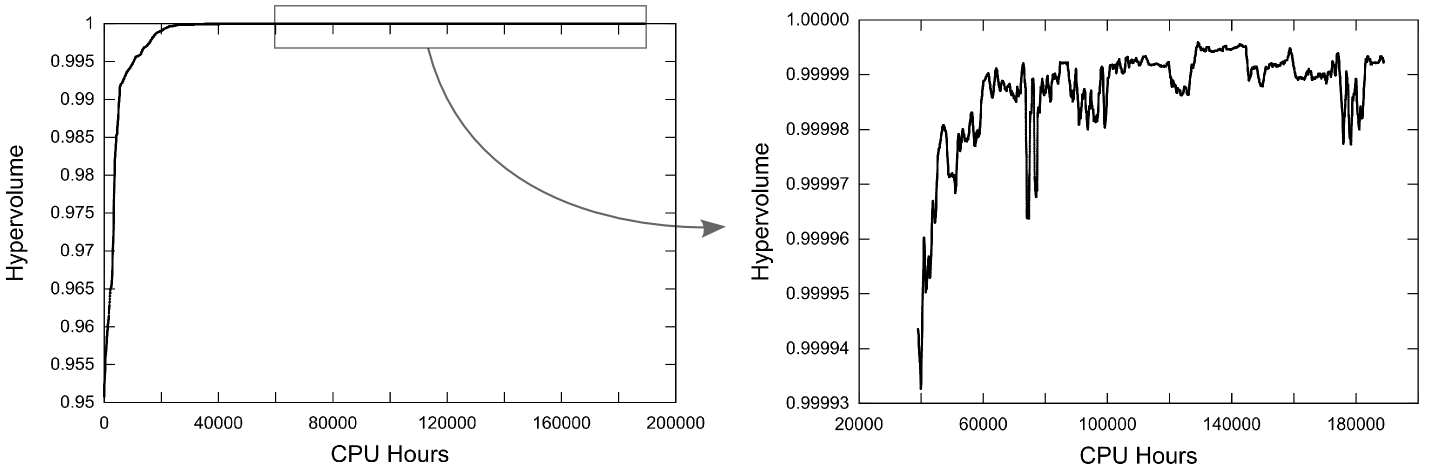
\includegraphics[width=1.0\linewidth]{half_billion_simulation_fig1_hypervolume.png}
  \end{sidecaption}
\end{figure}

After the convergence of the algorithm, $200$ different parameter settings were proposed as possible calibrated sets of parameter values. Because a set of $100$ executions can only provide an approximation of the objective scores of a parameter setting and because we want to make sure that they are well evaluated, $\num{10000}$ more executions of each proposed parameter setting were conducted. After recomputing the dominance selection, the dominated parameter set­ tings were excluded and $62$ parameter settings remained in the Pareto front. As stated above, a multiobjective exploration does not lead to the selection of a single optimized solution but leads to a set of possible candidates for the calibration: each set of parameter settings selected by the procedure represents a specific compromise on the three objectives. Thus, it is possible to distinguish among the parameter settings those satisfying only two objectives out of three from those which offer a better compromise on the three objectives without, however, reaching the best possible values on each objective. This configuration confirms that these three objectives are not redundant and that the procedure vacillates between them to find well-fitted parameter settings. Among the $62$ parameter settings of the Pareto front, some are less satisfying than others. We consider as unsuitable the parameter settings where at least one of the scores of the three objectives has a normalized error over $0.1$ (ie, over $10\%$ of error). Only $29$ parameter settings satisfy this new condition. The values estimated for each parameter of the $29$ selected sets are presented in table \ref{t:parametre}.


The analysis of this new subset shows interesting aspects. First, all of them correctly identify the order of magnitude of the only parameter of the model which can be roughly deduced from the initial conditions and the calibration objectives: the maximum resource parameter ($R_{max}$ ) which is used to limit the logistic growth of the population of each settlement \Anote{foot2}. Second, the four parameters whose values are a priori unpredictable (DistanceDecay, the parameter of dissuasion from the interactions by the distance; $P_{creation}$ , the probability of appearance of an innovation; $P_{diffusion}$ , the probability of its diffusion; and finally InnovationImpact, the impact of the innovation on the growth of the population) are estimated in a very small domain of variation compared with their possible domain of variation (table 3). The ratio between the estimated and theoretical volume defined by these five dimension domains is of \~ $\SI{4.7e-16}{} / \num{320000}{} = \SI{1.5e-21}{}$ ! What is remarkable is how the values taken by each parameter are all in a small neighbourhood, which suggests high reliability considering that they must be given those orders of magnitude to obtain plausible results while using the model for simulation. However it should be noted that the exact values estimated for each parameter do not have any absolute meaning. They only make sense all together, according to their interrelationships in the mechanisms of the model.

\begin{table}[H]
\begin{sidecaption}[fortoc]{Global domain of exploration and calibrated parameter value domain of variation.}[t:domain]
\centering
\begin{tabular}{@{}lll@{}}
\toprule
                   & Explored Domain & Solutions Domain          \\ \midrule
$P_{creation}$     & {[}0,1{]}       & ~{[} \SI{1.1e-06} ; \SI{1.3e-06} {]} \\
$P_{diffusion}$    & {[}0,1{]}       & ~{[} \SI{6.7e-07} ; \SI{6.9e-07} {]} \\
$InnovationImpact$ & {[}0,2{]}       & ~{[} \SI{7.7e-03} ; \SI{8.4e-03} {]} \\
$DistanceDecay$    & {[}0,4{]}       & ~{[} 0.66; 0.75 {]}       \\
$R_{max}$          & {[}1,40000{]}   & ~{[} 10090; 10465 {]}     \\
Volume             & 320000          & ~ \SI{4.7e-16}{}               \\ \bottomrule
\end{tabular}
\end{sidecaption}
\end{table}

Within the subset of $29$ parameter settings there is no way to prefer one setting over the others: the multiple executions of each setting lead to good results and acceptable variability of the outputs. Figures 2 and 3 give an example of such outputs. They depict the results produced by one of the parameter settings (in bold characters \Anote{foot3} in table 2). Figure 2 shows the evolution of the rank–size distribution of settlement sizes during a simulation of the parameter setting. This evolution corresponds to what is expected of the model: a progressive and continuous process of hierarchical organisation of the settlement system (the slope of the linear fit of the rank–size distribution shifts from $0.2$ to $0.9$ in $4000$ years for a maximum reached size reached of about $\num{10000}$ inhabitants). This result is quite robust if we consider the low variability of the recorded final state from one simulation to another (figure 3).


\begin{table}[!htbp]
\begin{sidecaption}[fortoc]{Calibrated parameter settings (rounded values).}[t:calibrated]
\resizebox{\columnwidth}{!}{%
\begin{tabular}{@{}llllllll@{}}
\multicolumn{5}{l}{Parameter setting}                                               & \multicolumn{3}{l}{\% error for each objective score}                                                                                                                                           \\ \midrule
$R_{max}$ & \begin{tabular}[c]{@{}l@{}}$Distance$ \\ $Decay$ \end{tabular}  & $P_{creation}$ & $P_{diffusion}$ &  \begin{tabular}[c]{@{}l@{}}$Innovation$ \\ $Impact$ \end{tabular} & \begin{tabular}[c]{@{}l@{}}distribution \\ objective\end{tabular} & \begin{tabular}[c]{@{}l@{}}population \\ objective\end{tabular} & \begin{tabular}[c]{@{}l@{}}time \\ objective\end{tabular} \\ \midrule
$\num{10464}$     & $\num{0.691}$           & \SI{1.11e-06}{}       & \SI{7.90e-07}{}        & $\num{0.0077}$                        & $\num{2.02}$                                                 & $\num{6.59}$                                                            & $\num{1.00}$                                                      \\
$\num{10465}$     & $\num{0.709}$           & \SI{1.14e-06}{}       & \SI{7.88e-07}{}        & $\num{0.0078}$                        & $\num{2.04}$                                                 & $\num{7.31}$                                                            & $\num{0.10}$                                                      \\
$\num{10459}$     & $\num{0.705}$           & \SI{1.15e-06}{}       & \SI{7.92e-07}{}        & $\num{0.0077}$                        & $\num{2.22}$                                                 & $\num{6.98}$                                                            & $\num{0.48}$                                                      \\
$\num{10465}$     & $\num{0.708}$           & \SI{1.15e-06}{}       & \SI{7.86e-07}{}        & $\num{0.0078}$                        & $\num{2.51}$                                                 & $\num{6.00}$                                                            & $\num{0.40}$                                                      \\
$\num{10261}$     & $\num{0.679}$           & \SI{1.17e-06}{}       & \SI{7.78e-07}{}        & $\num{0.0078}$                        & $\num{2.79}$                                                 & $\num{5.29}$                                                            & $\num{4.55}$                                                      \\
$\num{10262}$     & $\num{0.679}$           & \SI{1.15e-06}{}       & \SI{7.52e-07}{}        & $\num{0.0078}$                        & $\num{2.95}$                                                 & $\num{5.00}$                                                            & $\num{2.15}$                                                      \\
$\num{10262}$     & $\num{0.665}$           & \SI{1.14e-06}{}       & \SI{7.24e-07}{}        & $\num{0.0078}$                        & $\num{2.99}$                                                 & $\num{5.53}$                                                            & $\num{1.23}$                                                      \\
$\num{10261}$     & $\num{0.683}$           & \SI{1.12e-06}{}       & \SI{7.38e-07}{}        & $\num{0.0080}$                        & $\num{3.1 }$                                                 & $\num{4.34}$                                                            & $\num{1.15}$                                                      \\
$\num{10260}$     & $\num{0.699}$           & \SI{1.17e-06}{}       & \SI{7.38e-07}{}        & $\num{0.0079}$                        & $\num{3.62}$                                                 & $\num{5.51}$                                                            & $\num{0.20}$                                                      \\
$\num{10287}$     & $\num{0.690}$           & \SI{1.23e-06}{}       & \SI{7.56e-07}{}        & $\num{0.0078}$                        & $\num{3.63}$                                                 & $\num{3.74}$                                                            & $\num{3.46}$                                                      \\
$\mathbf{\num{10259}}$     & $\mathbf{\num{0.688}}$           & $\mathbf{\SI{1.20e-06}{}}$       & $\mathbf{\SI{7.41e-07}{}}$        & $\mathbf{\num{0.0079}}$                        & $\mathbf{\num{3.74}}$                                                 & $\mathbf{\num{3.55}}$                                                            & $\mathbf{\num{2.48}}$                                                      \\
$\num{10169}$     & $\num{0.736}$           & \SI{1.29e-06}{}       & \SI{7.39e-07}{}        & $\num{0.0079}$                        & $\num{4.90}$                                                 & $\num{5.20}$                                                            & $\num{0.03}$                                                      \\
$\num{10205}$     & $\num{0.683}$           & \SI{1.19e-06}{}       & \SI{7.42e-07}{}        & $\num{0.0082}$                        & $\num{5.10}$                                                 & $\num{2.60}$                                                            & $\num{6.03}$                                                      \\
$\num{10126}$     & $\num{0.738}$           & \SI{1.22e-06}{}       & \SI{7.61e-07}{}        & $\num{0.0082}$                        & $\num{5.69}$                                                 & $\num{2.88}$                                                            & $\num{1.50}$                                                      \\
$\num{10126}$     & $\num{0.738}$           & \SI{1.24e-06}{}       & \SI{7.39e-07}{}        & $\num{0.0082}$                        & $\num{6.02}$                                                 & $\num{3.08}$                                                            & $\num{0.55}$                                                      \\
$\num{10096}$     & $\num{0.701}$           & \SI{1.14e-06}{}       & \SI{7.14e-07}{}        & $\num{0.0084}$                        & $\num{6.12}$                                                 & $\num{2.58}$                                                            & $\num{1.55}$                                                      \\
$\num{10169}$     & $\num{0.736}$           & \SI{1.29e-06}{}       & \SI{7.39e-07}{}        & $\num{0.0080}$                        & $\num{6.25}$                                                 & $\num{2.46}$                                                            & $\num{1.20}$                                                      \\
$\num{10165}$     & $\num{0.734}$           & \SI{1.29e-06}{}       & \SI{7.24e-07}{}        & $\num{0.0080}$                        & $\num{6.31}$                                                 & $\num{2.91}$                                                            & $\num{0.30}$                                                      \\
$\num{10121}$     & $\num{0.732}$           & \SI{1.28e-06}{}       & \SI{7.41e-07}{}        & $\num{0.0081}$                        & $\num{6.41}$                                                 & $\num{2.36}$                                                            & $\num{1.90}$                                                      \\
$\num{10164}$     & $\num{0.735}$           & \SI{1.29e-06}{}       & \SI{7.27e-07}{}        & $\num{0.0080}$                        & $\num{6.45}$                                                 & $\num{2.74}$                                                            & $\num{0.45}$                                                      \\
$\num{10103}$     & $\num{0.733}$           & \SI{1.24e-06}{}       & \SI{7.42e-07}{}        & $\num{0.0084}$                        & $\num{7.67}$                                                 & $\num{1.90}$                                                            & $\num{3.10}$                                                      \\
$\num{10092}$     & $\num{0.736}$           & \SI{1.29e-06}{}       & \SI{7.14e-07}{}        & $\num{0.0082}$                        & $\num{7.81}$                                                 & $\num{2.22}$                                                            & $\num{1.10}$                                                      \\
$\num{10098}$     & $\num{0.737}$           & \SI{1.29e-06}{}       & \SI{7.12e-07}{}        & $\num{0.0082}$                        & $\num{7.84}$                                                 & $\num{2.55}$                                                            & $\num{0.58}$                                                      \\
$\num{10094}$     & $\num{0.741}$           & \SI{1.28e-06}{}       & \SI{7.12e-07}{}        & $\num{0.0083}$                        & $\num{8.46}$                                                 & $\num{1.99}$                                                            & $\num{1.00}$                                                      \\
$\num{10129}$     & $\num{0.737}$           & \SI{1.29e-06}{}       & \SI{7.07e-07}{}        & $\num{0.0082}$                        & $\num{8.64}$                                                 & $\num{1.97}$                                                            & $\num{0.68}$                                                      \\
$\num{10110}$     & $\num{0.735}$           & \SI{1.28e-06}{}       & \SI{6.77e-07}{}        & $\num{0.0083}$                        & $\num{9.04}$                                                 & $\num{2.48}$                                                            & $\num{0.03}$                                                      \\
$\num{10091}$     & $\num{0.744}$           & \SI{1.31e-06}{}       & \SI{7.25e-07}{}        & $\num{0.0083}$                        & $\num{9.22}$                                                 & $\num{1.51}$                                                            & $\num{2.68}$                                                      \\
$\num{10091}$     & $\num{0.741}$           & \SI{1.31e-06}{}       & \SI{7.12e-07}{}        & $\num{0.0083}$                        & $\num{9.61}$                                                 & $\num{1.49}$                                                            & $\num{2.15}$                                                      \\
$\num{10109}$     & $\num{0.734}$           & \SI{1.28e-06}{}       & \SI{6.79e-07}{}        & $\num{0.0084}$                        & $\num{9.64}$                                                 & $\num{1.77}$                                                            & $\num{0.18}$                                                      \\ \bottomrule
\end{tabular}%
}
\end{sidecaption}
\end{table}

\begin{figure}[!htbp]
\begin{sidecaption}[fortoc]{Evolution of the rank–size distribution during a simulation of one of the best calibrated parameter settings.}[fig:S_ranksize]
  \centering
 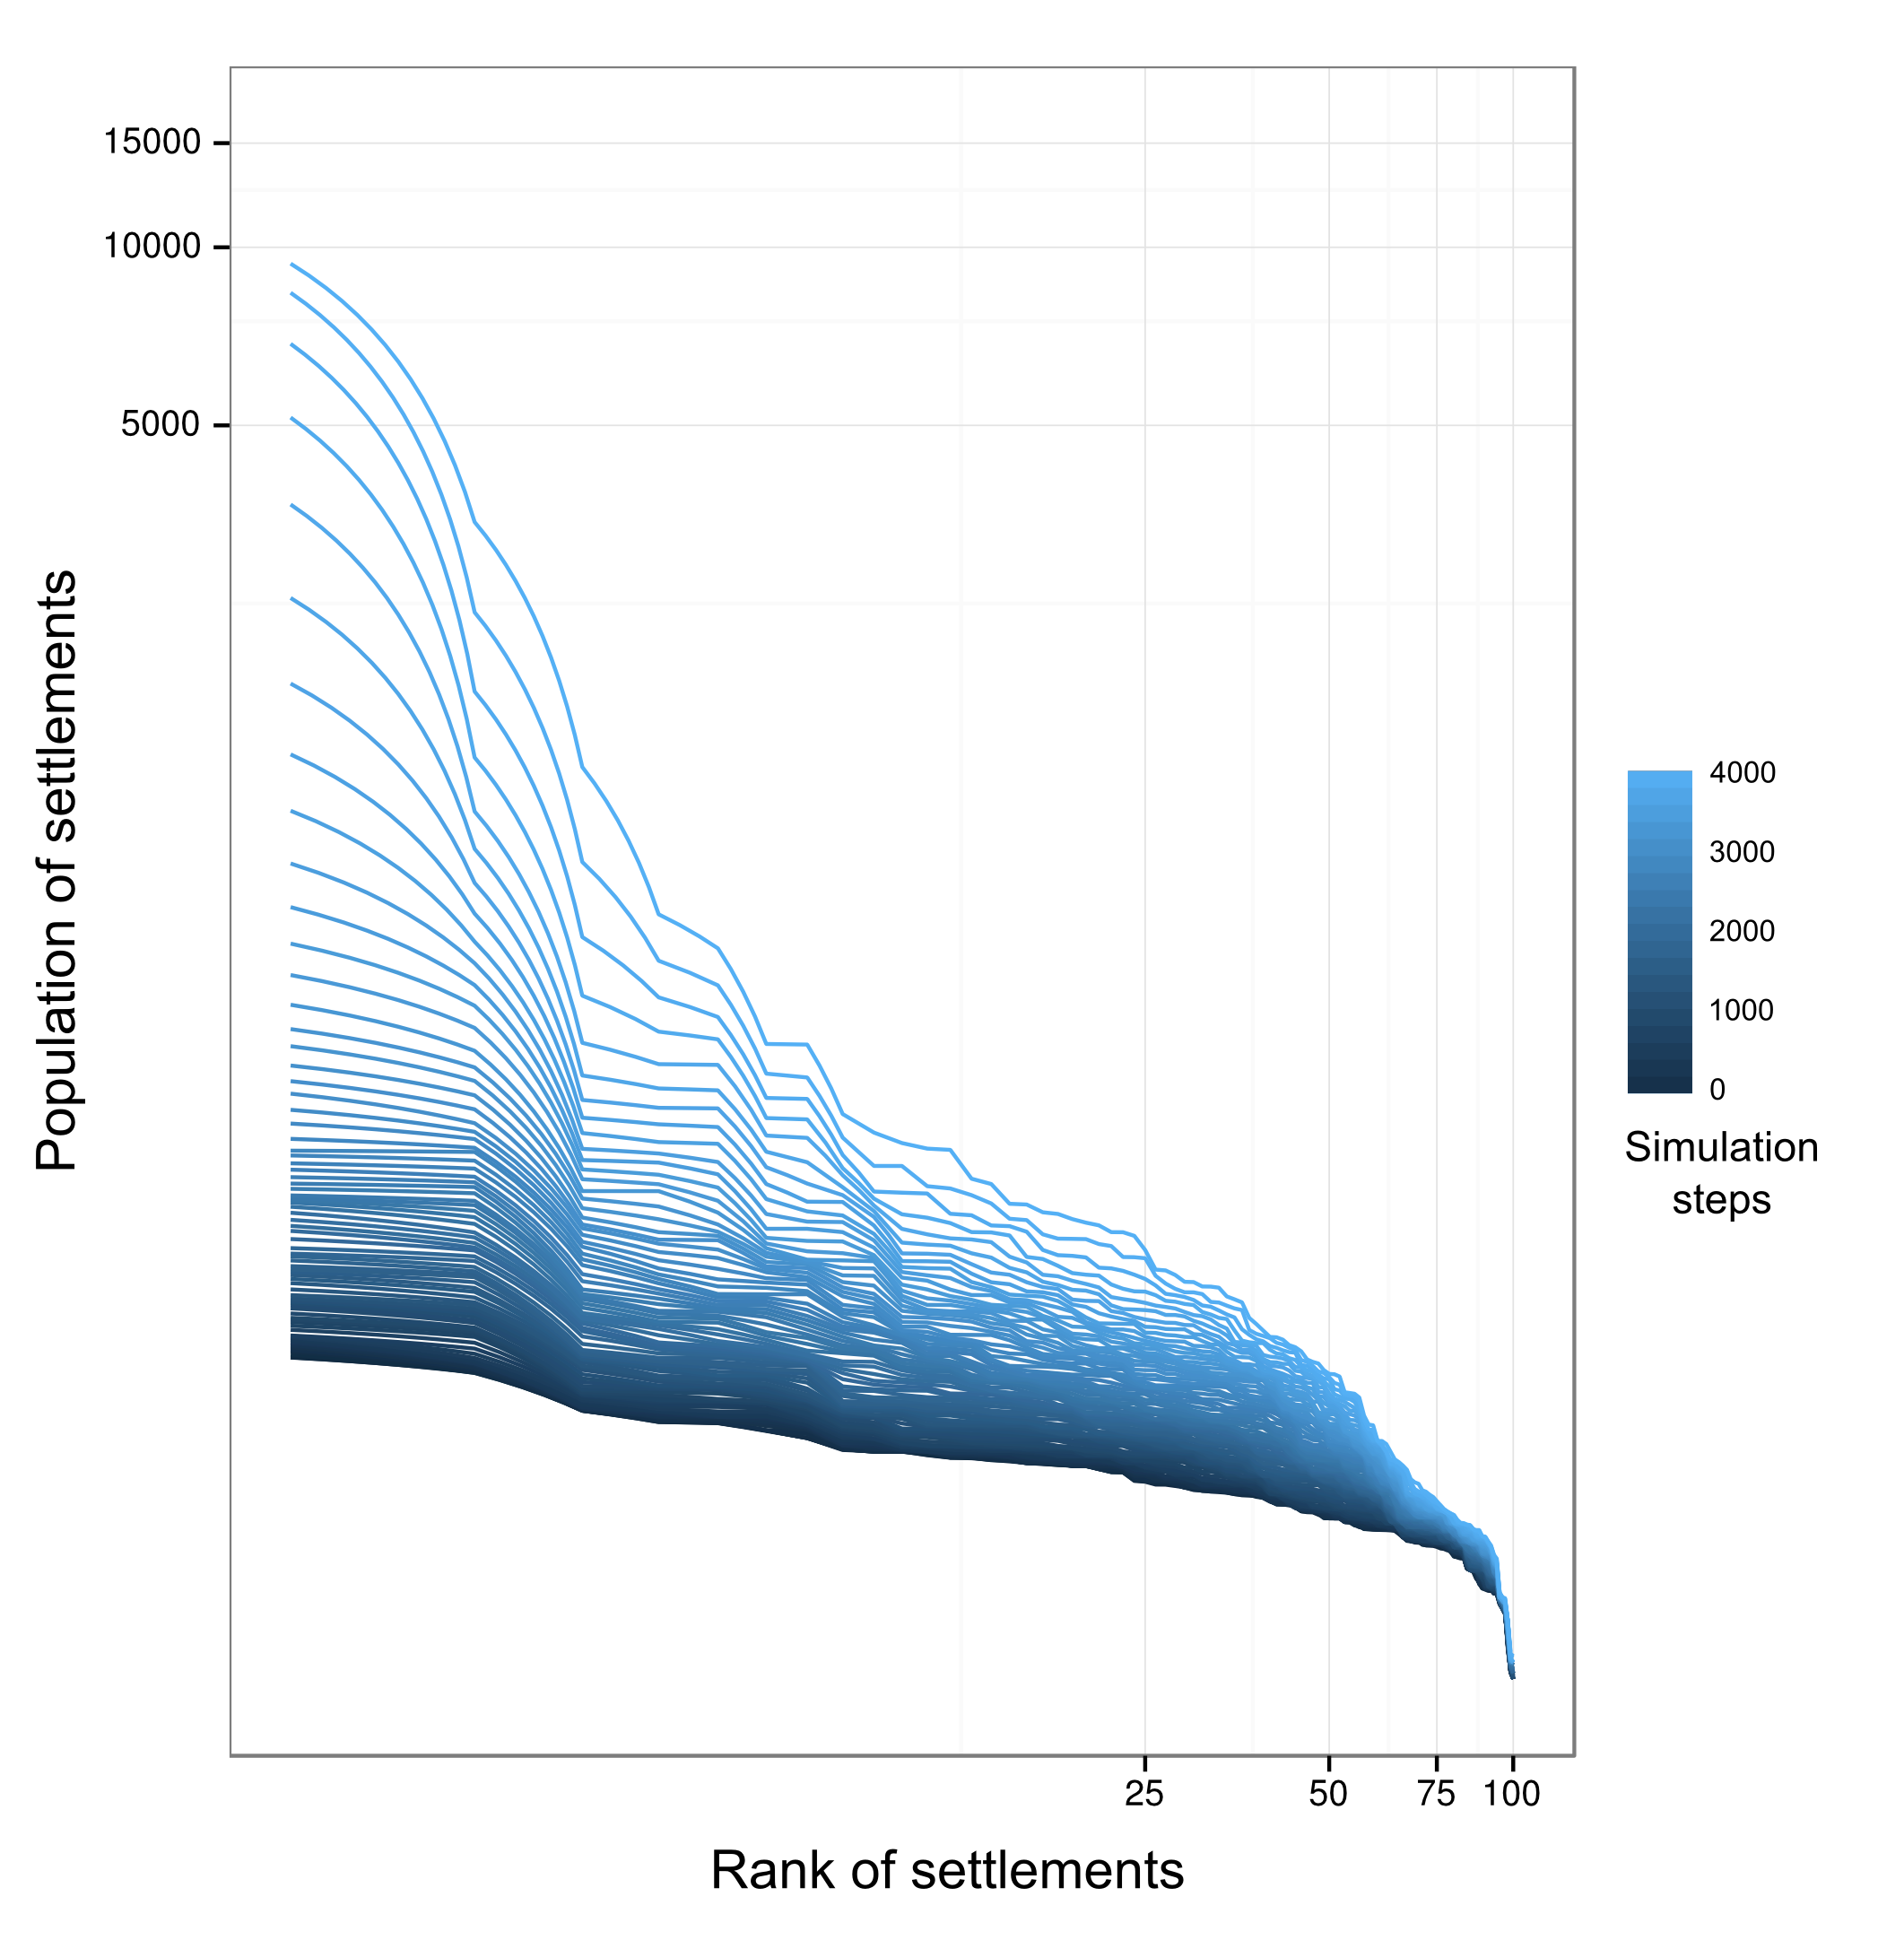
\includegraphics[width=1.0\linewidth]{RTbleu.png}
  \end{sidecaption}
\end{figure}

\begin{figure}[!htbp]
\begin{sidecaption}[fortoc]{Variability of the rank–size distribution at the final simulation step in 100 simulations of one of the best calibrated parameter settings.}[fig:S_hypervolumemedian]
  \centering
 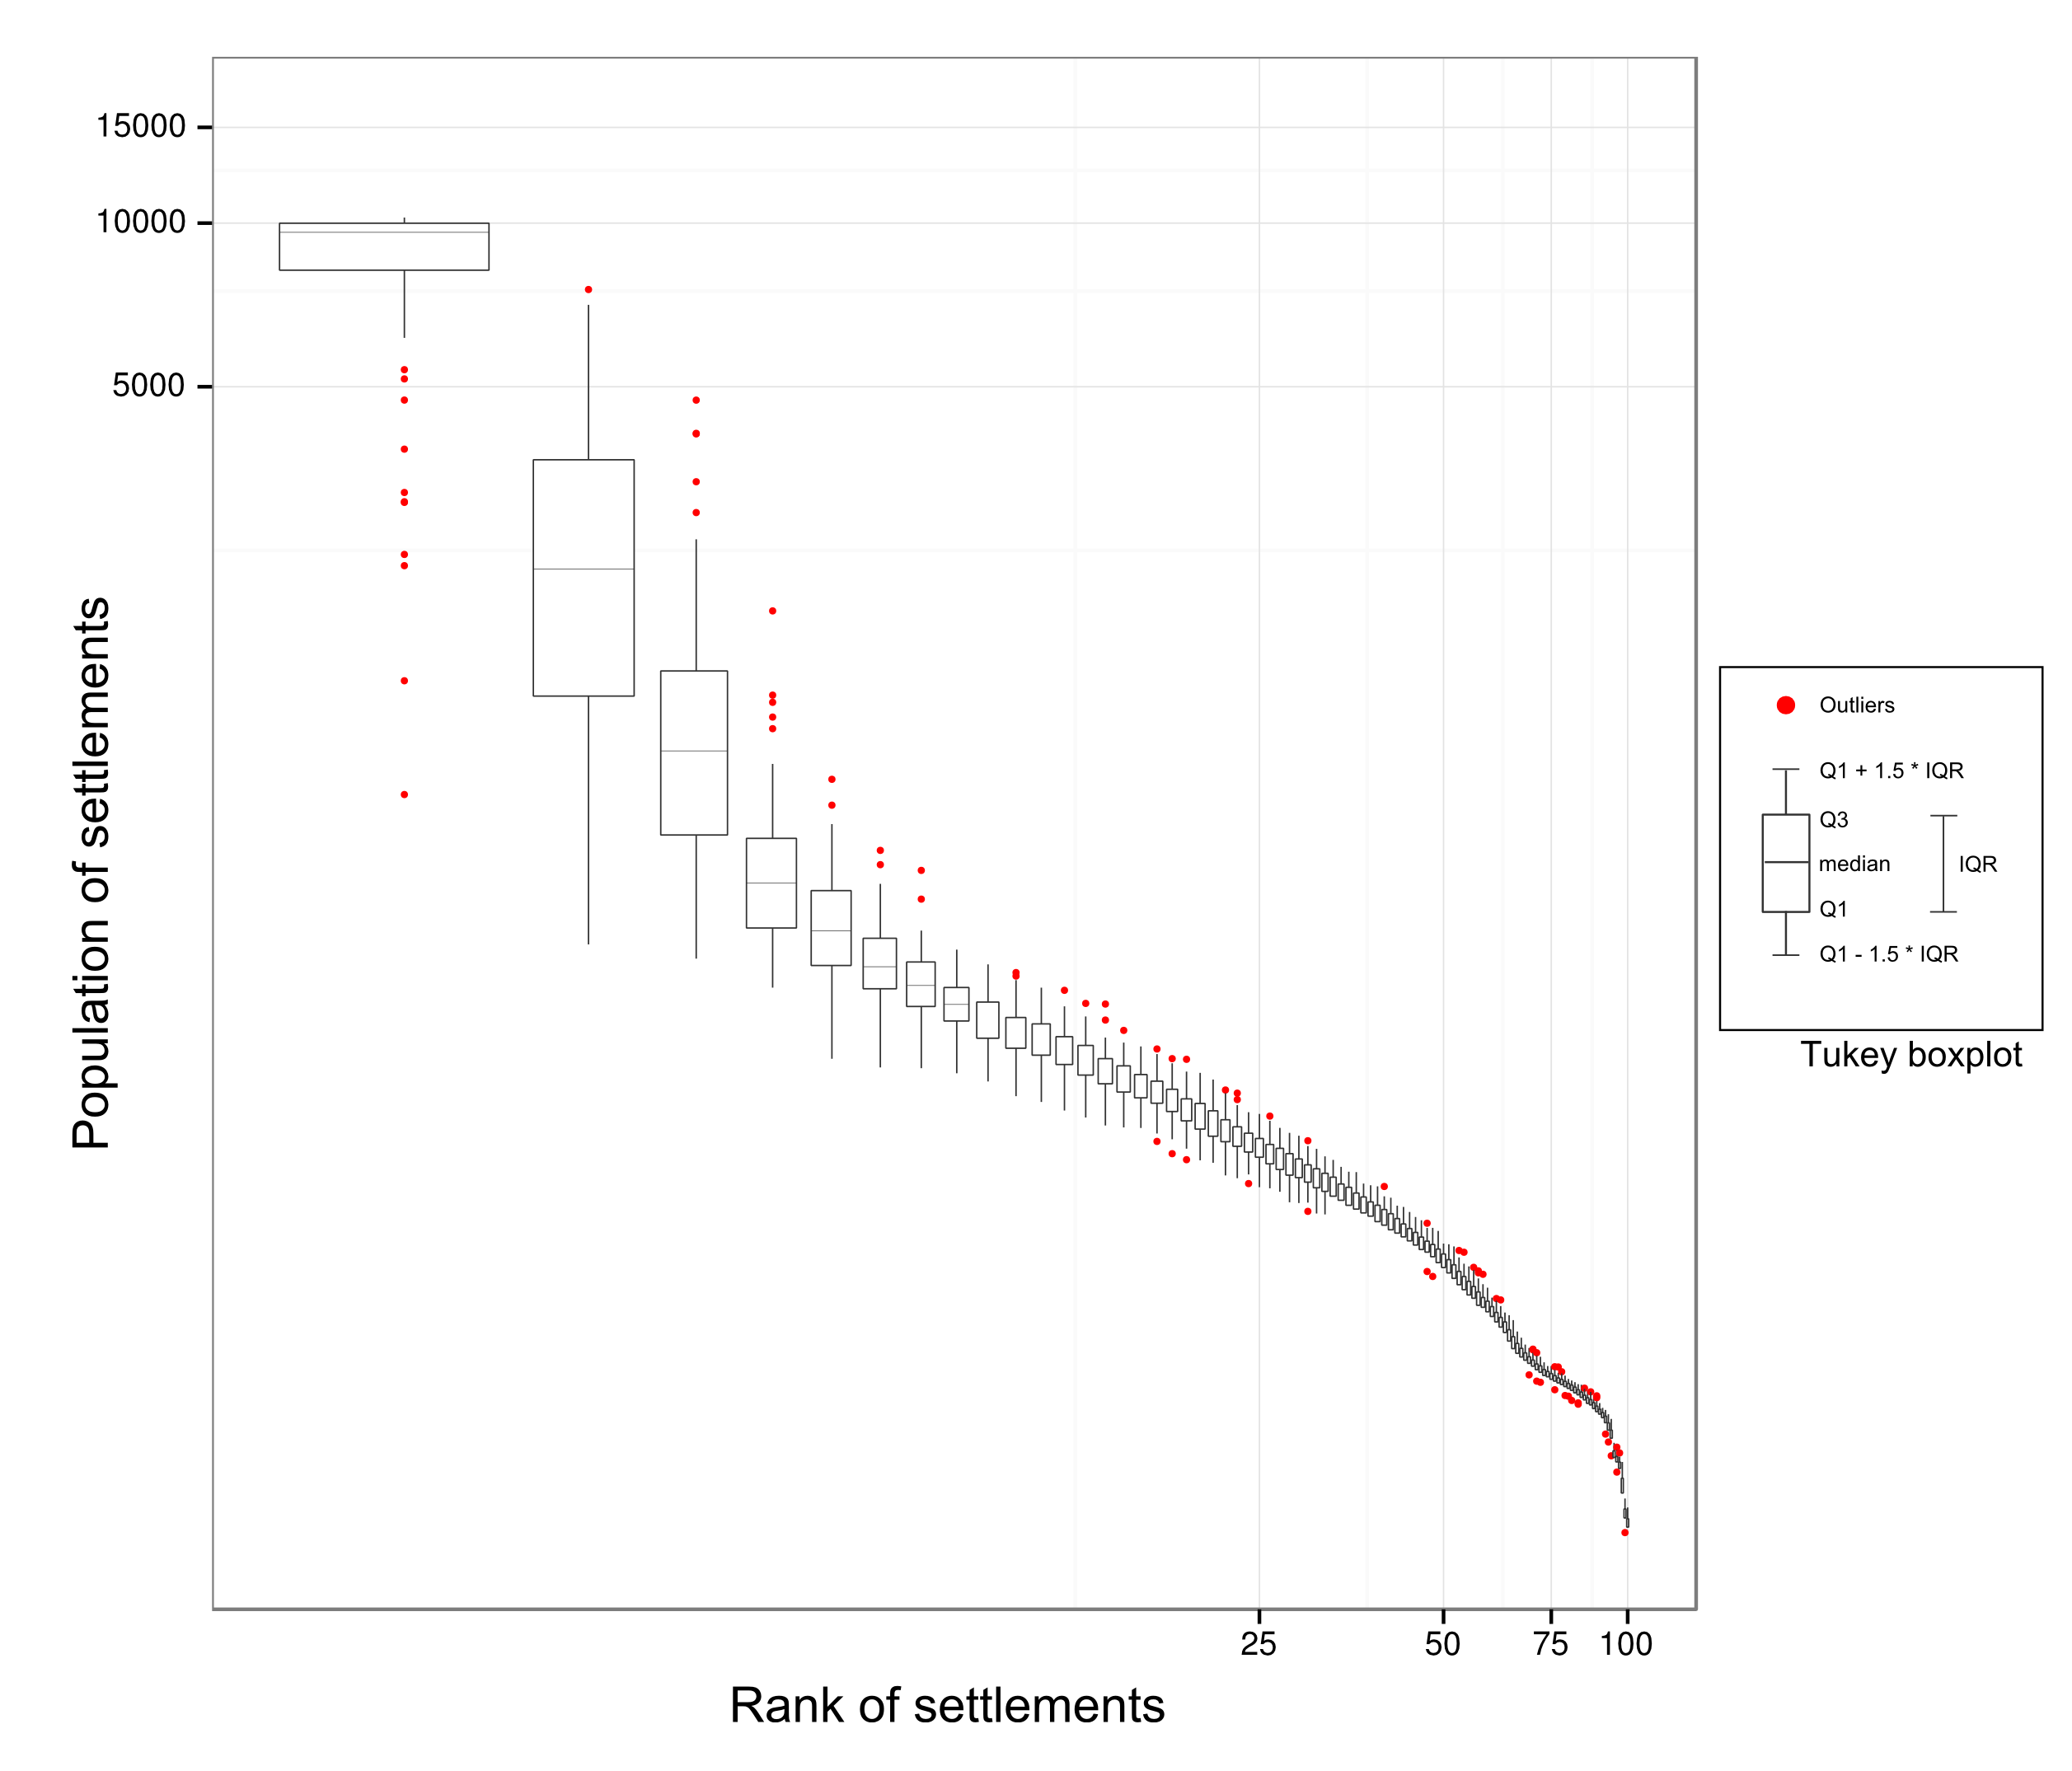
\includegraphics[width=1.0\linewidth]{varRTrouge.png}
  \end{sidecaption}
\end{figure}

\section{Conclusion}
\label{sec:conlusion}

An automatic calibration procedure was applied for the first time on a multiagent model, SimpopLocal, which was developed to simulate the emergence of a system of urban settlements. It provides convincing results to solve the calibration problem for multiagent models. With five parameters whose value could not be estimated from empirical data, it would have been quite difficult to find an estimation of a calibrated parameter setting ‘manually’. By reversing this calibration problem into an optimisation problem, our automated calibration procedure generates parameter settings which reproduce the stylized facts embodied in three objective functions very well. This enables us to confirm a decisive advance in the validation of this model: we proved that the SimpopLocal model, as conceived in its simplicity, is able to satisfactorily generate a plausible evolution including the emergence of an urban hierarchy. and quantifying criteria for evaluating the model; a methodology for exploring the parameter space with an automated process using evolutionary algorithms; a technical protocol for reducing the exploration time by massive distributed computing. The application of these principles to modelling not only improves the quality of communication about the model, but also ensures the repeatability of its experimentation and contributes to creating accessible modelling tools that can be shared via the free and open-source software tool for model experiments. OpenMOLE ( \href{http://www.openmole.org}{http://www.openmole.org}) . In order to help the dissemination of these techniques, we published several tutorials on the developed tools. For example, on how to design a grid exploration of a NetLogo model \Anote{foot4} and how to explore a NetLogo model with evolutionary algorithms. \Anote{foot5} This work forges a path for other modellers, who could use a similar data-intensive grid-based approach in their modelling experiments.

\textbf{Acknowledgments.} This work is funded by the ERC Advanced Grant Geodivercity, the Agence de l’Environnement et la Maitrise de l’Energie, the network Réseau de Recherche sur le Développement Soutenable, and the Institut des Systèmes Complexes Paris Île-de-France. Results obtained in this paper were computed on the biomed and the vo.complex-system.eu virtual organization of the European Grid Infrastructure ( http://www.egi.eu ). We thank the European Grid Infrastructure and its supporting National Grid Initiatives (France-Grilles in particular) for providing the technical support and infrastructure. We also thank an anonymous reviewer for help in improving the first version of the paper.

\section{Annexe}
\label{sec:annexe}

\begin{figure}[!htbp]
\begin{sidecaption}[fortoc]{Diagramme de classe}[fig:S_classe]
  \centering
 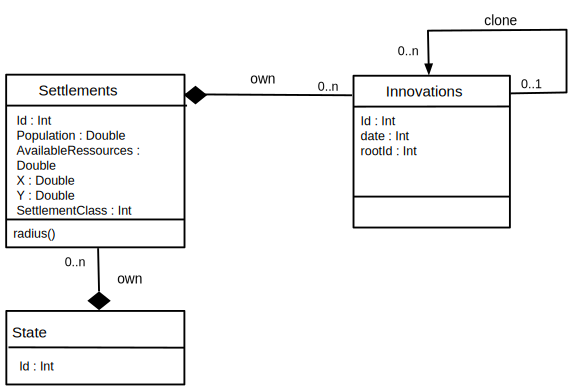
\includegraphics[width=1.0\linewidth]{slocal_uml.pdf}
  \end{sidecaption}
\end{figure}

\begin{figure}[!htbp]
\begin{sidecaption}[fortoc]{Diagramme d'activité principal}[fig:S_activite]
  \centering
 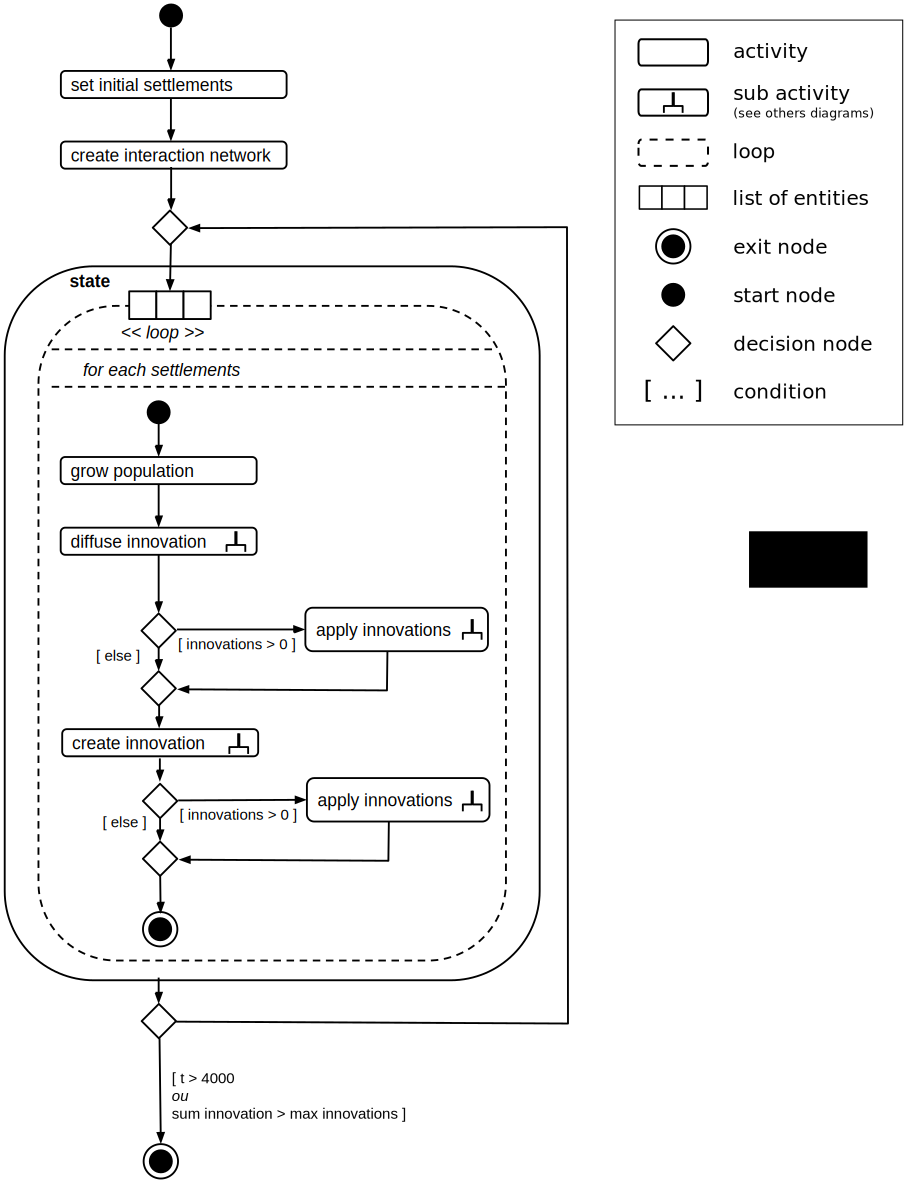
\includegraphics[width=0.9\linewidth]{slocal_state.pdf}
  \end{sidecaption}
\end{figure}

\begin{figure}[!htbp]
\begin{sidecaption}[fortoc]{Diagramme d'activité pour la gestion des innovations}[fig:S_activite]
  \centering
 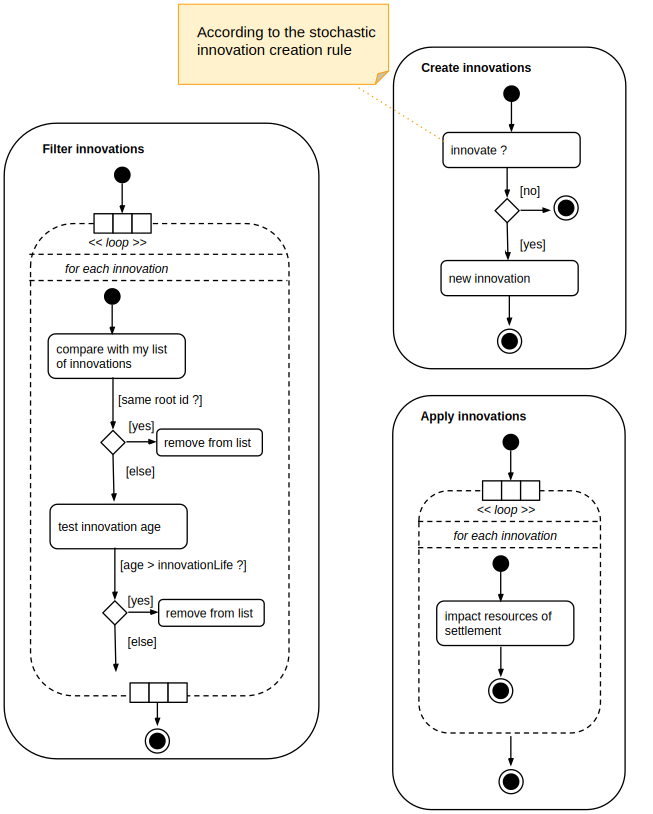
\includegraphics[width=1.0\linewidth]{slocal_groupeinov.pdf}
  \end{sidecaption}
\end{figure}

\printbibliography[heading=subbibliography]


% -*- root: These.tex -*-

%%ENTRETIENT
\chapter{Entretiens}
\label{chap:entretiens}

\section{Entretien avec le professeur historien et médiéviste Jean-Philippe Genet}
\label{sec:entretient_genet}

\noindent\textbf{- Entretien réalisé le : } 13 mai 2015 \\
\noindent\textbf{- Transcription faite le :} 14 mai 2015 \\
\noindent\textbf{- Validation faite le :} en attente de confirmation, la version définitive apparaitra dans quelques semaines dans la version de la thèse déposée sur Internet.

\paragraph*{Sébastien Rey : Si vous pouviez m'en dire plus sur le type de matériel, l'ouverture du centre ?}

\noindent\emph{Jean-Philippe Genet}: Le centre je ne l'ai connu que quand je suis revenu ici. J'ai été assistant à la Sorbonne en 1967, et à l'époque il n'y avait pas encore Paris 1, c'était la Sorbonne, tout était donc ensemble. Je n'ai pas entendu de suite parler d'informatique, en tout cas chez les historiens. Il y avait bien des historiens qui en faisaient à cette époque, mais ils n'en faisaient pas ici, ou alors dans des endroits relativement, disons, je dirais occultes. A ma connaissance, les deux personnes qui s'intéressaient à l'informatique à l'époque, donc en 1967, c'était surtout \textbf{Antoine Prost}, qui travaillait dans le centre d'histoire contemporaine, qui à l'époque réunissait le dix-neuvième et le vingtième siècle. Il y avait aussi, quelqu'un, je pense qu'il était déjà là, je n'en suis pas absolument sûr, qui s'appelait \textbf{William Serman}. Et donc il faisait de l'analyse de discours, avec un informaticien qui s'appelait \textbf{Édouard Cadet}, un Haïtien, un type très bien, je l'ai un peu fréquenté. Je savais que cela existait, mais on ne pouvait pas être au courant si on n’appartenait pas spécifiquement à ce centre-là, il n'y avait pas d'activité en cours.
Donc ensuite j'ai fait mon service militaire complet à Paris 1, c'était en douce, et après je suis parti à Oxford pendant un an. Quand je suis rentré, je me suis mis sérieusement à l'informatique, j'ai donc pris des cours et çà je l'ai fait à Paris 5. J'ai suivi les cours de \textbf{Marc Barbut}, et puis des gens qui étaient dans son équipe. J'ai ensuite commencé à me préoccuper pour en faire  dans le cadre de mes recherches. A ce moment-là, je n'avais pas vraiment entendu parler du centre de calcul de Paris 1, et c'est seulement à l'automne 70 que je me suis vraiment préoccupé de faire quelque chose. Alors, ce que j'ai trouvé à ce moment-là durant l'année 70-71, c'est un ordinateur qui a été remplacé très rapidement, un IBM classique assez poussif. Il a été remplacé rapidement par une machine qui était un  Philips P880.

\paragraph*{Sébastien Rey : Ce numéro vous a marqué en tout cas.}

\noindent\emph{Jean-Philippe Genet}: Oui, car celui-là on a beaucoup travaillé dessus. On avait deux types d'activités : de la prosopographie (analyse de biographie avec des méthodes statistiques y compris l'analyse factorielle) faite sur le P880, et puis je faisais de l'analyse lexicale sur les grosses machines d'Orsay sur des crédits des CNRS, sur lesquelles on pouvait passer la nuit, ou le samedi et le dimanche. J'avais une Diane à l'époque, que je chargeais de bac de cartes perforées, je les trainais sur le sol, et puis on allait passer le samedi jusqu'à ce que mort s'ensuive à Orsay. On travaillait en mode batch, vous lancez l'exécution et vous attendez le retour, qui est une erreur en général. Une virgule qui manque quelque part, vous cherchez la faute, vous la corrigez, et puis vous relancez jusqu'à ce que ça finisse par passer. La grande différence par rapport à ce qu'on faisait en local, c'est que pour travailler à Orsay, il fallait des crédits CNRS.

\paragraph*{Sébastien Rey : Cela coûtait cher pour l'époque ?}

\noindent\emph{Jean-Philippe Genet}: Ce n’est pas que c'était très cher, mais il fallait surtout demander au comité national du CNRS l'autorisation, et obtenir un crédit, faire un dossier, etc. bref c'était compliqué. Donc je l'ai fait, j'ai obtenu un crédit, je m'en souviens très bien, mon premier crédit était de mille francs, et je recevais un carnet de chèques. C'était très bien d'ailleurs, la gestion n'était pas très compliquée, mais ça marchait très bien. Ceci dit cela ne servait à rien dans le cas d'Orsay, puisque là c'était des virements internes, donc je n’ai jamais touché au carnet de chèques. Avec ce travail à Orsay on est monté en puissance, on est devenu une vraie équipe CNRS,  puis un laboratoire du CNRS (date?). Tout cela a pris beaucoup d'importance et bientôt on n'était plus obligé d'aller à Orsay, et on a pu travailler au Laboratoire Informatique des Sciences de l'Homme.

\paragraph*{Sébastien Rey : Donc à la MSH, au LISH}

\noindent\emph{Jean-Philippe Genet}:Voilà, à la MSH, boulevard Raspail, c'est là que j'ai connu Philippe Cibois.

\paragraph*{Sébastien Rey : À quelle date environ ? }

\noindent\emph{Jean-Philippe Genet}: Cela doit être dans les années 75-80, franchement je suis très mauvais sur les dates, je suis médiéviste alors tout ça ... je vois plus loin :)

Par contre pour tout le travail, disons sur les bases de données, on travaillait sur le Philips P880, et c'est là où il y avait un club d'utilisateur assez restreint. En économie il y avait Pierre-Yves Hénin, et une personne qui s'appelait \textbf{Pouchain} qui était un économiste qui travaillait avec \textbf{Hénin}. Il y avait les trois géographes \textbf{Thérése Saint Julien}, \textbf{Denise Pumain}, et puis un spécialiste de la France qui s'appelait \textbf{Yvan Chauviré} je crois. Il est resté à Paris 1 assez longtemps, mais il n'y est plus maintenant.


\paragraph*{Sébastien Rey : Ça donc, c'était l'équipe de base ?}

\noindent\emph{Jean-Philippe Genet}: Oui l'équipe de base, et puis il y avait d'autres utilisateurs, bien sûr, mais le fonctionnement était assez bon grâce à cette équipe. Il y avait le dieu tutélaire qu'on ne voyait jamais qui passait de temps en temps, un économiste, qui était vital, car c'était de lui que dépendait le centre, et puis comme il était très respecté chez les économistes ... il s'appelait \textbf{Claude Fourgeaud}. Celui-ci était un professeur d'économie déjà âgé, qui avait déjà eu une attaque, un peu bizarre comme ça, mais c'était un universitaire, semble-t-il très fort et en tout cas très respecté. Ce qui fait que le centre de calcul a toujours eu les moyens qu'il lui fallait. La tête pensante pour les machines, les ingénieurs, etc. c'était \textbf{Édouard Valensy}. Celui-ci enseignait à Paris 1, mais c'était un général polytechnicien, qui s'occupait du centre de recherche de l'armée à Saclay, et qui avait donc cette grande qualité de nous fournir en informaticiens quand on voulait travailler sur des projets scientifiques, des gens d'une très très grande qualité intellectuelle. Pour éviter le problème d'aller à Orsay, j'ai pu développer justement mon logiciel d'analyse lexicale avec deux garçons : \textbf{Jacques Mondelli} qui est devenu un cadre très important chez Bull, et qui est mort malheureusement de la maladie de l'amiante, car les centres de calcul à l'époque n'étaient pas non plus des endroits très sains. Et François Hucher qui a travaillé par la suite à la C2I. L'un était de l'école des mines Berkeley, et l'autre était Centralien. Donc évidemment c'était des gens qui étaient à la pointe du combat en informatique, et on a pu faire vraiment à ce moment-là du bon travail. Bien qu'ayant des moyens dérisoires. Le centre de calcul lui-même c'était toujours le P880, ici à Paris 1. Celui qui le faisait tourner pour nous surtout, c'était un gars qui s'appelait \textbf{Xavier Debanne}. Je crois qu'il est devenu catholique convaincu, il est parti à Rome en tout cas et il a fondé plus ou moins une boîte, et il a travaillé plus ou moins avec le Vatican. Il travaillait à cette époque avec \textbf{Jean-Paul Trystram}, quelqu'un qui était un prof un peu inclassable, ayant également fait un manuel d'informatique pour les sciences sociales. \textbf{Xavier Debanne} avait développé pour un logiciel qui s'appelait BDP2 (banque de données paris 1 version 2), devenu ensuite BDP3, jusqu'à BDP4, et qui marchait très bien. En gros c'était un SPSS miniature, mais qui vous permettez de faire tous les tests, tout çà sur cartes perforées. On faisait ça avec le P880, car il tolérait d'assez gros fichiers, donc on pouvait traiter des bases de données importantes, faire des tris croisés, des analyses factorielles, et tout ça c'était quand même pas mal. 

Le centre de calcul était organisé ainsi, il y avait la salle avec l'ordinateur, et à côté il y avait une petite salle où les dames  faisaient les perforations. Il y avait deux perforeuses, et puis nous, enfin tous les chercheurs, on se faisait les perforations nous-mêmes la plupart du temps. 

\paragraph*{Sébastien Rey : Denise m'a également parlé de ces deux dames.}

\noindent\emph{Jean-Philippe Genet}: C'était les piliers de la maison, elles avaient leur franc-parler, et c'était assez pittoresque, surtout une. Et elles ne s'envoyaient pas dire quand quelqu'un faisait une erreur, cela fusait. 
 
\paragraph*{Sébastien Rey : Donc celles-ci étaient employées à plein temps.}

\noindent\emph{Jean-Philippe Genet}: Oui elles faisaient des petits trous toute la journée, avec une vitesse évidemment qu'enviaient beaucoup les malheureux qui faisaient leurs cartes perforées eux-mêmes.

\paragraph*{Sébastien Rey : Vous savez jusqu'à quand ça a duré ?}

\noindent\emph{Jean-Philippe Genet}: Tout ça a duré assez longtemps, car le CNRS a beaucoup renâclé à pousser la micro-informatique. C'est çà un des problèmes, d'ailleurs Cibois vous en a peut-être parlé.

\paragraph*{Sébastien Rey : Oui c'est arrivé vers les années 1980 - 1984, plutôt sur initiative de quelques personnes.}

\noindent\emph{Jean-Philippe Genet}: C'était beaucoup dans le cadre du CRH (centre de recherche historique). Enfin, il y avait certaines personnes qui connaissaient les universités américaines, et qui dès lors qu'elles sont revenues en France ont dit à ce moment-là \enquote{ça ne va pas} . Moi de mon point de vue, je n'étais même pas au courant. J'ai découvert ça presque un peu tard. Ici à Paris 1 on n’avait pas de micro-ordinateur, on travaillait toujours sur le P880, et surtout on n’avait pas les logiciels, donc on continuait à travailler avec le logiciel BDP4 qui fonctionnait bien. J'avais mon système qui s'appelait ALINE pour l'analyse linguistique qui fonctionnait également bien, donc je n'allais pas changer pour des micro-ordinateurs pour lequel il n'y avait aucun logiciel. D'ailleurs le CNRS ne nous y encourageait pas, il ne voulait pas nous donner d'argent pour qu'on achète des micro-ordinateurs, c'était explicite. Et parce que'il voulait surtout continuer à nous faire financer. En fait il donnait aux équipes des sciences humaines des crédits, pour faire de l'informatique, mais ces crédits étaient ensuite convertis automatiquement en crédits reversés au centre de calcul du CIRCE à Orsay. En fait l'argent ne faisait qu'un détour par nous, il tournait en rond et revenait dans leur système. Donc il ne nous poussait pas du tout à faire de la micro-informatique. Sans compter qu'évidemment on est toujours méfiant, dès que le fonctionnaire va se trouver autonome, il va regarder YouTube, enfin à l'époque ça n’existait pas. À l'époque le truc le plus « in », c'était vous savez les balles de tennis qui rebondissent, pong ... Donc il fallait que l'on continue à travailler avec les grosses machines.

Tout çà a quand même eu une fin. De toute façon j'avais déjà commencé à faire de l'enseignement de l'informatique pour les historiens à Paris 1. J'ai dû commencer dans les années 1977-78 quand les deux logiciels commençaient à bien tourner. La difficulté c'est que comme on n’avait pas de micro-ordinateur, on allait en procession rue cujas jusqu'au bâtiment de la fac de droit pour faire du batch sur le Philips P880.

\paragraph*{Sébastien Rey : Le Philipps était situé où dans le bâtiment ?}

\noindent\emph{Jean-Philippe Genet}: Quand vous rentrez au panthéon, vous voyez la cour, vous allez au coin droit, vous rentrez dans le bâtiment, et c'était là juste à droite. Au pied du grand escalier qui monte, c'était là, les trois-quatre pièces qui étaient là. Ce n’était pas grand.
Il y avait d'autres gens qui faisaient de l'informatique à Paris 1, par exemple \textbf{Colette Roland}, mais elle ne s'est jamais intéressée à ça, je ne l'ai jamais vu travailler sur une machine du centre. Elle faisait plus de la théorie informatique. La seule personne qui vraiment a été l'âme du centre, et qui l'a fait fonctionner, c'était \textbf{Yvonne Girard}, une mathématicienne. C'est elle qui a assuré le fonctionnement du centre pendant de longues années.

Je ne me souviens plus de l'année exacte 1984-85, mais  il y a \textbf{Jean-Pierre Bardet}, un historien démographe de Paris 4, qui a été ensuite au ministère de la Recherche. Un jour il en a eu marre de tout ça, car à Paris 4 c'était pire, nous on avait un centre de calcul, mais eux il en avait à peine. \textbf{Jean-Pierre Bardet} travaillait beaucoup au LISH, et je travaillais avec lui. On lui avait même prêté nos machines pour imprimer sa thèse, car la sienne était tombée en panne la veille de la soutenance, le type d'événement qui crée des liens. Et quand il s'est trouvé au ministère, \textbf{Jean-Pierre Bardet} a changé tout ça. Il a envoyé aux départements d'histoire, un petit peu partout en France, des micro-ordinateurs. C'était des Bull 45, à l'époque c'était bien, c'était des PC de base si vous voulez. Et il en a envoyé 12 à Paris 1 à l'UFR d'histoire. Le directeur de l'époque c'était \textbf{Robert Fossier}, cela tombait bien, car j'étais très proche de lui, et celui-ci ne savait pas trop quoi en faire. On a d'abord pensé distribuer les ordinateurs aux professeurs, et puis en fait ils n'étaient pas vraiment intéressés parce que la plupart ne savaient pas à quoi ça servait. Donc moi j'ai dit qu'il fallait trouver un endroit où les mettre tous ensemble, pour lancer ensuite un enseignement d'histoire et informatique. De façon plus solide, car cette fois-ci au lieu d'aller au panthéon, on fera l'enseignement sur place. \textbf{Robert Fossier} a dit d'accord, et on a donc cherché un local, que l'on a trouvé au sous-sol, là où il y a les salles d'informatique encore aujourd'hui. On a équipé la première avec ces Bull 45 et on a alors pu commencer une formation disons plus systématique pour les historiens. Il y avait à l'époque un bon prétexte, qui a disparu malheureusement par la suite, qui était l'existence de ce que l'on appelait un DEUG et une Licence MAS (mathématiques appliquées aux sciences sociales). 

\paragraph*{Sébastien Rey : Une formation qui a disparu il n'y a pas si longtemps non ?}

\noindent\emph{Jean-Philippe Genet}: Enfin si, en fait cela fait un bon moment. En tout cas les historiens en ont été exclus depuis un bon moment. Puisqu'en fait le gros du public c'était des économistes. Mais avec les collègues géographes justement on avait réussi à obtenir un quota, on avait droit à deux ou trois historiens, ou deux ou trois géographes, pour les intégrer à la formation. Et donc on était bien obligé de leur fournir une UV d'informatique appliquée à l'histoire, et il y en avait également une appliquée à la géographie. Et du coup l'idée a été simplement d'ouvrir cette UV d'informatique appliquée à l'histoire à d'autres étudiants qu'à ceux qui étaient seulement pour le DEUG MAS. Ce qui a permis d'avoir un effectif  assez vite important, car cela a plu aux étudiants. À la fin des années 1990, on a rendu ensuite rendu ça quasiment obligatoire dans l'UFR d'histoire. Cela fait partie de la licence, où il y a une série d'UV spécifiquement d'informatique. De toute façon c'est obligatoire, car il faut que les étudiants aient le C2I et des choses comme ça.

Et donc l'existence du centre de calcul, je suis sorti du cadre du centre de calcul stricto censu, mais voilà, cela a été le point de départ de tout çà. Je pense que cela a été vraiment utile jusqu'aux années 1985, et même peut-être après, mais évidemment quand on est passé à la micro-informatique, c'est devenu beaucoup moins intéressant et à Orsay il a pratiquement disparu. Tant que les micro-ordinateurs étaient très chers, évidemment cela avait son utilité, moi le premier Apple que j'ai acheté, je m'en souviens, car cela m'avait coûté très cher. À l'époque on achetait son ordinateur sur fonds propres, car il n'y avait pas de crédit recherche; les crédits recherches c'est une belle chose, mais ça date d'Allègre. Avant les années 1999-2000, on n’avait pas de grands budgets, et donc on s'achetait nous-mêmes nos ordinateurs. Le premier que j'ai acheté il m'en a coûté plus de 10000 francs, l'équivalent de 1500 euros. C'était un Apple 48K de mémoire, ça ne faisait pas grand-chose par rapport au Philips en comparaison. Vous rentriez une disquette avec un alphabet et puis les 4 accents, car vous aviez droit à seulement 4 caractères accentués. Ensuite le contenu était chargé en mémoire, et vous pouviez rentrer une disquette pour écrire et copier ce que vous faisiez. C'était des disquettes souples, là aussi on ne rentrait pas grand-chose. Ceci dit cela permettait de faire un certain travail. En histoire il y a une thèse qui a été faite expressément avec ce type d'appareil, qui le revendique, et qui a accepté les limitations pour montrer qu'on pouvait faire du bon travail. C'est la thèse de \textbf{André Sitzberg} sur les galériens. C'est un ouvrage important sur le plan historique. Celui-ci a quand même dépouillé tous les registres du bagne de Toulon, il a eu les données sur plus de 60000 galériens, qui ont permis une démonstration fondamentale c'est-à-dire de démontrer que les galériens ne servaient à rien. Ils étaient essentiellement là pour faire peur, et imposer la majesté du roi, et à travers la majesté du roi, assurer la rentabilité des fermes, des tabacs, et la gabelle puisque les galériens avant tout, ce ne sont pas des brigands, ce sont uniquement des gens qui essayaient de frauder sur le sel, le tabac, et puis il y avait aussi les déserteurs. Et ils ne ramaient pas du tout pour faire la guerre,  ils ramaient pour montrer que les galères étaient très belles. Si on n'avait pas eu les 60000 fiches, cette démonstration n'aurait pas pu exister. C'est une thèse qui a eu un vrai résultat historique, et avec un Apple 48K. Alors évidemment les gens ont protesté, et ils ont dit \enquote{ah ouais, vous avez codé les métiers alors les charpentiers il y a 50 dénominations possibles, il y a des tas de différences et on ne peut plus les retrouver}. Avec un 48K on faisait ce que l'on pouvait.

Ensuite j'ai acheté un ordinateur de cette série-là, pour l'équivalent de 2000 à 3000 euros. Alors tant que les ordinateurs étaient comme ça - il n'y avait pas de portable - le centre de calcul a gardé son intérêt, et les gens allaient travailler sur les micro-ordinateurs du centre de calcul. Ils ont remplacé assez vite le P880  par des micro-ordinateurs et les étudiants allaient travailler dessus. On pouvait utiliser ces micro-ordinateurs comme terminaux pour envoyer à Orsay, et travailler sur les logiciels installés là-bas. 
 Je ne sais pas jusqu'à quand les ordinateurs du centre de calcul ont été utilisés, car j'ai cessé de les utiliser, car à partir du moment où on était CNRS j'allais au LISH en cas de besoins plus importants. Le LISH a assez vite coulé, et Philippe Cibois est même venu à la rescousse à un moment pour le diriger.

\paragraph*{Sébastien Rey : En effet il semblerait qu'il y ait eu plusieurs directeurs successifs au LISH dans les années 80}

Celui qui a vraiment engagé le bras de fer, c'est \textbf{Michaël Hainsworth}. C'était un égyptologue, et donc en tant qu'égyptologue, il avait une grosse protection, car il faisait la partie informatique du travail de \textbf{Jean Leclant}, qui est devenu très vite le secrétaire perpétuel de l'institut. Autant dire qu'il avait le bras plus que long. Fort de cette protection, \textbf{Michaël Hainsworth} a essayé d'imposer un développement de la micro-informatique en accès libre très rapide, et ça a posé problème rapidement, car la direction du CNRS ne voulait pas lâcher la bride. Je le sais d'autant plus, car à l'époque j'étais à la direction scientifique du CNRS, et j'ai donc assisté de près au clash entre Hainsworth avec qui je travaillais, et les gens de la direction scientifique. Une direction censée être de gauche, ouverte, mais les réflexes administratifs français ... La priorité du CNRS, les physiciens y veillaient, c'était les gros équipements, c'était le CIRCE, et il ne fallait surtout pas aider le LISH à pousser et à éparpiller la micro-informatique chez les utilisateurs.  

\paragraph*{Sébastien Rey : À partir de là, ça a décliné ?}

\noindent\emph{Jean-Philippe Genet}: Les laboratoires se sont équipés, et les centres se sont déplacés. Les centres de calcul comme le LISH, comme le CIRCE, comme celui de Paris 1, c'était des endroits formidables, car on travaillait tous ensemble. Et on avait du temps, car on attendait les résultats. Donc quand on se trompait, c'était la consultation générale, qu'est-ce-que ça peut être, etc.. Il y avait un échange réel ! J'ai revu plusieurs fois \textbf{Denise Pumain}, car j'ai été président du comité de la section histoire, et par la suite je l'ai aussi croisée dans toutes les instances, mais je n'ai plus jamais parlé avec elle comme je pouvais parler quand on se disait \enquote{mince, qu'est-ce qui n'a pas marché cette fois-ci ?}. C'est là que se faisait le vrai travail, c'est là où on pouvait vraiment discuter. \textbf{Philippe Cibois} a été une aide précieuse pour tous les gens qui ont importé, car c'était un des esprits les plus clairs que je connaisse dans le domaine de l'informatique. \textbf{Michaël Hainsworth} aussi, c'était des gens avec qui on pouvait vraiment travailler. Et puis quand il y avait vraiment de gros problèmes, il y avait des mathématiciens ou des physiciens, qui avaient un niveau informatique d'un niveau bien plus élevé encore.

\paragraph*{Sébastien Rey : Le CIRCE mettait également une littérature grise, des écoles d'étés, des formations également non ? }

\noindent\emph{Jean-Philippe Genet}: Il y avait tout çà oui, mais après il fallait avoir du temps. Je n'étais pas personnel CNRS, mais oui j'en ai fait quelqu'unes, comme celle sur les Analyses Factorielles au CIRCE. Quand j'ai commencé, j'ai fait du Fortran, mais je n'ai jamais été capable de programmer des choses trop ardues. J'ai tout de suite vu que si l'on voulait programmer un logiciel d'analyse lexicale, ce n'était pas la peine d'essayer sans aide extérieure. Ce que \textbf{Jacques Mondelli} et \textbf{François Hucher} ont fait, c'était de l'informatique de très haut niveau. Il était passé par l'école des mines et l'école centrale, pas moi. Ils connaissaient par exemple toute une série de tests statistiques qui permettaient de ranger les lemmes par ordre alphabétique en gagnant du temps, et surtout de l'espace mémoire, car à l'époque les contraintes étaient très grandes, donc ils avaient des tas d'astuces statistiques pour faire avancer plus rapidement la conception des logiciels. 
 

\paragraph*{Sébastien Rey : C'était donc du travail main dans la main avec les informaticiens ?}

\noindent\emph{Jean-Philippe Genet}: J'ai des amis qui ont programmé des analyses factorielles, des choses comme çà. On avait des modèles que l'on pouvait réadapter. Mais quand on prend un système comme BDP4, c'est vraiment un logiciel de base de données, qui est entièrement paramétré, vous rentrez les données, et après vous pouvez faire beaucoup de choses. C'est un peu ce que l'on peut faire aujourd'hui avec des logiciels comme R, que l'on peut adapter à son propre usage, mais à l'époque il n'y avait rien de tel. 

\paragraph*{Sébastien Rey : SPSS arrive dans les années 1976 ? }

\noindent\emph{Jean-Philippe Genet}: Il y a une version pour les gros systèmes, c'est celle que tout le monde a utilisée. Il y avait trois logiciels de ce type que l'on utilisait : SPSS, SAS, BMD (biometrical data). Maintenant il y a des versions pour micro-ordinateurs. On pouvait déjà rentrer des fichiers concernant plus de 80000 individus. Le problème c'est que cela coûtait cher, car il fallait les acheter ces logiciels, et Paris 1 ne les avait pas. Il n'y avait pas de crédit recherche. À partir de 1998-99, il y a eu des crédits recherche, et il y a également eu tous ces masters professionnels qui ont rapporté de la taxe d'apprentissage. Les économistes ont par exemple eu très vite de gros moyens. En base de données, ils travaillaient sur Oracle, alors que nous en histoire, en géographie, on n’a jamais pu atteindre le niveau suffisant pour travailler sur Oracle, le standard aujourd'hui dans les entreprises. La question des moyens certes demeurait, mais à partir de 1998-99, on était passé dans un monde différent, cela marchait beaucoup mieux.

\paragraph*{Sébastien Rey : Et pour la formation en Fortran chez les historiens ? } 

\noindent\emph{Jean-Philippe Genet}: Ah non, chez les historiens on y a renoncé très vite. J'ai pu relancer les choses quand on a été vraiment équipés en micro-ordinateur, et à ce moment-là j'ai essayé d'obtenir des postes. Ainsi il y a eu la possibilité, dans les années 1995 - 1996, d'obtenir des postes de PRAG. On a réussi à créer quatre postes, et un de ces postes a été transformé par la suite en poste de maître de conférences. À l'heure actuelle, il y a 4 PRAG, et un maître de conférences, et il devrait y avoir un cinquième, car on a été obligé de le lâcher pour faire de l'enseignement de statistiques. On devrait le récupérer plus tard sous une forme statistiques/informatiques. Cela fait quand même 6 postes qui ont été créés, et donc qui n'ont pas été pris sur les contingents existants. Si j'ai quand même réussi quelque chose dans la vie, c'est ça, vous êtes trop jeune pour savoir ça, mais faire créer un poste dans l'université, c'est difficile. Ce ne sont pas forcément de bons postes, car ils ne sont que PRAG, mais c'est mieux que rien. Et cela a permis de développer cet enseignement à l'informatique. Je crois que les autres disciplines ont fait de même, il y a des PRAG informatiques ailleurs.

\paragraph*{Sébastien Rey : L'enseignement informatique s'est-il transformé pour devenir seulement l'activité de « bonne  utilisation des logiciels » ?  }

\noindent\emph{Jean-Philippe Genet}: C'est plus que çà, c'est vraiment un enseignement d'histoire. On essaye de développer depuis le niveau de la problématique, de voir ce qu'il est possible de faire face aux sources, ce que l'informatique va vous permettre de faire par la suite. Ce qui suppose d'avoir déjà une idée sur la façon de faire, notamment pour les traitements statistiques. De même, si vous voulez faire des traitements lexicologiques, il faut que vous ayez déjà une petite idée sur la linguistique, sur la lexicologie, la sémantique quantitative, et qu'est-ce qu'on peut tirer d'un contexte. De même pour la prosopographie. J'avais conçu cet enseignement de cette façon, et je crois qu'ils l'ont gardé ainsi, comme une formation pour l'informatique par la recherche. C'est-à-dire, après 3 ou 4 mois de cours magistraux et de rodage sur les logiciels pour qu'ils sachent les utiliser, on demande aux étudiants de chercher un sujet de recherche. Ils fabriquent de petites bases de données, sur des bases textes, sur des choses variées : les menus de Louis XV, le discours des présidents de conseil général de l'Orne, la date d'arrivée des clubs de football dans la première division en France, la programmation des cinémas parisiens entre telle date et telle date, etc. Les étudiants cherchaient quelque chose et il fallait que cela soit eux qui le trouvent, et à partir de là, on leur disait : ou vous construisez une base de données de type BDP4, SAS, SPSS , ou vous faites un traitement textuel avec une base texte sur laquelle vous allez faire des traitements linguistiques. Vraiment un enseignement par la recherche. C'était le travail de base, et ça a un peu évolué par la suite, car c'était en licence. On a remi quelque chose de plus banal pour faire le C2I basique.

\paragraph*{Sébastien Rey : Effectivement le C2I c'est un enseignement de base, une utilisation finalement assez passive de l'informatique.}

\noindent\emph{Jean-Philippe Genet}: On a surtout beaucoup rajouté derrière. C'est ce qu'on a probablement fait de plus intéressant. On a fait des séminaires au niveau de la maîtrise, qui sont des vrais cours d'informatique, par exemple on apprend à programmer du XML, à travailler sur BDP5, à faire du SIG, etc

\paragraph*{Sébastien Rey : et le logiciel R ?}

\noindent\emph{Jean-Philippe Genet}: R, non car c'était la partie statistique, mais on essaie de s'y remettre avec Stéphane Lamassé. Celui-ci  qui permet de travailler justement avec R, qui est adapté aux données historiques. On essaye de fabriquer des choses qui facilitent le travail pour les historiens. Et puis on a créé des ateliers, des séminaires, de suivis des thèses, et des maîtrises. En maîtrise c'est obligatoire, tous les étudiants doivent faire un semestre d'informatique, et s'ils prennent vraiment un traitement informatique dans le cadre de leur maîtrise, ils ont droit à un suivi individuel, même chose pour les thèses. C'est très bien, mais également très prenant.

\paragraph*{Sébastien Rey : Si on revient sur le centre de calcul de Paris 1 , avant l'installation des micro-ordinateurs, y avait-il eu des terminaux ? }

\noindent\emph{Jean-Philippe Genet}: Non non, il fallait aller au Philips, ou alors on allait au LISH, mais ça ne marchait pas pour l'enseignement, c'était uniquement pour la recherche. 

Je ne les ai pas utilisés, je ne me rappelle pas. Comme nous avons eu nos propres micro-ordinateurs, on a cessé d'utiliser ces salles. Et surtout, \textbf{Jean-Paul Trystram} a pris sa retraite, et \textbf{Xavier Debanne} est parti. Xavier c'était un type curieux, il a été en cinquième ou sixième année de médecine. Puis, il a plaqué la médecine, il a fondé sa boîte d'informatique, et il est parti en Italie, pour je ne sais quelle raison.

\paragraph*{Sébastien Rey : Ces postes n'ont pas été remplacés ?}

\noindent\emph{Jean-Philippe Genet}: Ce n'était pas vraiment des postes, je ne sais pas vraiment comment ils étaient payés. Ils devaient être vacataires ou quelque chose comme ça. Les gens qui travaillaient ici, \textbf{Hucher}, \textbf{Mondelli}, c'étaient des gens que je payais avec des vacations CNRS. Ils faisaient leur service militaire en réalité. Cela nous venait par \textbf{Édouard Valensy} qui les avait recrutés à Saclay et travaillaient pour lui. Comme ils n'avaient pas un énorme travail à réaliser pour l'armée, ils se faisaient un peu d'argent en travaillant ici. On travaillait surtout le soir ou la nuit. 

Il se trouve que je suis devenu ami avec \textbf{Hucher} et \textbf{Mondelli}, et donc après on a continué à travailler ensemble, mais c'est devenu difficile... Je me suis battu en particulier pour \textbf{Jacques Mondelli}, Dieu sait que si j'avais pu le faire ça aurait pu lui sauver la vie puisqu'il est mort à cause de l'amiante. J'ai essayé de le faire nommer ici. Il sortait des mines, il avait un doctorat de Berkeley. Ils n'ont pas voulu de son doctorat, et il lui ont dit \enquote{ok, on vous prend, mais il faut que vous repassiez un doctorat ici}.

Après des années de lutte, j'ai fini par obtenir un poste, converti depuis un poste de sergent de pompier. C'est quand même un type qui travaillait avec nous, qui s'appelait \textbf{Marc Turket}, probablement encore en poste au centre de calcul. C'était un archéologue qui avait fait de l'informatique, et qui a travaillé avec \textbf{Olivier Buchsenschutz}. Ce dernier travaillait sur la carte archéologique de la Gaule, une grosse base de données des archéologues au CNRS. Il était rattaché ici, à l'UFR d'art et d'archéologie de Paris 1.

\textbf{Marc Turket} était un spécialiste des ossements. Donc évidemment il faisait des classifications automatiques à n'en plus finir. Il était assez compétent. Mais bon, il avait peu d'espoir de trouver un poste dans le monde de l'archéologie, donc il s'est contenté d'un poste pas très bien payé, mais qui lui permettait de continuer à faire de l'informatique, au centre de calcul.

\paragraph*{Sébastien Rey : Le centre de calcul, qu'est-il devenu par la suite ? }

\noindent\emph{Jean-Philippe Genet}: Je sais plus ce que c'est devenu, de toute façon cela dépendait des économistes, de l'UFR 2. Les économistes ont dû remettre la main sur les locaux. Tout ce qui était interdisciplinarité, centré sur l'usage informatique a disparu avec la micro-informatique. Vous avez cité \enquote{ le médiéviste et l'ordinateur }, ça marchait très très bien. Du jour où il y a eu la micro-informatique, le déclin a été continu. On avait une association qui s'appelait \textit{International Association for History and Computing}  basée en Angleterre. J'en ai été le premier président, cela marchait très bien, on a fait d'importants colloques. Mais passé 1995, tout ça a disparu. Il y avait la branche française dont s'occupait \textbf{André Sitzberg} qui avait un bulletin publié par le LISH, ça a également disparu. Tout ça est fini. La seule chose qui surnage de cette époque, c'est parce qu'on s'était refusé à faire de l'informatique, c'était la revue Histoire et Mesure. Une revue qui était au CNRS, mais qui est retenue aujourd'hui par le CRH de l'école des hautes études.

\paragraph*{Sébastien Rey : Donc si je résume bien, de 69 à 85 vous étiez actif au centre de calcul.}

\noindent\emph{Jean-Philippe Genet}: C'est ça, disons 1970-71, je ne sais plus exactement quand cela a commencé. On peut même dire jusqu'à 90, il me semble, mais ma chronologie est très floue.

\paragraph*{Sébastien Rey : vous connaissez des travaux de recherches qui étudient cette période du centre de calcul à Paris 1 ? }  

\noindent\emph{Jean-Philippe Genet}:Un étudiant de Toulouse, \textbf{Castex} , mais il n'a pas fini sa thèse. 

\paragraph*{Sébastien Rey : Avez-vous participé au « bulletin des messaches » de la FMSH ?}

\noindent\emph{Jean-Philippe Genet}: On l'a effectivement lu, mais c'était vraiment du giron de la maison des sciences de l'homme, boulevard Raspail. On était un peu exclu de ce type de publication. A la maison des sciences de l'homme, le coeur de l'utilisation plus que les historiens, c'était surtout les sociologues. Parmi les historiens qui ont beaucoup fréquenté le LISH, il y avait  \textbf{André Sitzberg}, \textbf{Barbet}, \textbf{Laurent Ladury}. Mais voilà, par exemple, \textbf{Laurent Ladury} c'est pas lui qui a réalisé la partie informatique de son travail, c'est \textbf{Sitzberg} qui a principalement travaillé pour lui. Il y avait donc des gens qui travaillaient pour les autres. Par exemple c'est \textbf{Jules Roméro}, le premier enseignant en histoire et informatique ici, qui a fait toutes les thèses de Paris 4. Par conséquent, il n'a pas pu faire la sienne. C'est assez injuste. \textbf{Hainsworth} lui a été viré, voilà ce qui arrive finalement aux gens qui ont compté.

\textbf{Philippe Cibois} je l'ai surtout connu quand il était au LISH. Je le voyais pour ses logiciels à lui. J'utilise d'ailleurs toujours son logiciel tri-deux, c'est le seul auquel je fais vraiment complètement confiance.


\paragraph*{Sébastien Rey : Au niveau de la pratique des centres de calculs, y a-t-il encore un usage du calcul intensif chez les historiens ? }

\noindent\emph{Jean-Philippe Genet}: Non, je ne vois pas trop pour quels usages ... \\

\textit{... pause de quelques secondes ...}
\\
\noindent\emph{Jean-Philippe Genet}: \textbf{Denis Pechanski} a lancé un très gros programme franco-américain qui est appuyé sur le mémorial de Caen, et puis sur les projets muséaux qui entourent le 11 septembre aux Etats-Unis. Dans leurs projets, il y en avait un plus axé sur la visite du musée et les moyens de mesurer l'attention. Là il y avait du très gros calcul. En ce moment de mon côté, on fait un répertoire des membres des écoles et de l'université parisienne au moyen âge, c'est gros parce que ce sont des fiches textes, on en a 16000 en stock, 8000 accessibles en ligne, vous pouvez regarder. Pour certains de ces personnages, cela représente plus de 100 pages à imprimer : Albert Legrand, Thomas Daquin, etc. C'est énorme au niveau des données, mais au niveau des calculs c'est finalement assez banal,  des tris croisés, des analyses factorielles. 

Il y a quelques projets qui utilisent les GIS et mobilisent des moyens de calculs, mais ce n'est pas non plus colossal. On a un gros projet sur le tracé des rues, et l'emplacement des maisons parisiennes. On travaille avec un laboratoire de La Rochelle. En partant de tracés du 19e siècle, on remonte le temps de façon régressive à partir de tout ce que l'on peut savoir sur la voirie, et cela jusqu'à ce que l'on n’ait plus aucun tracé.  On a éventuellement des relevés archéologiques, et surtout on a des registres de tailles pour les maisons. Donc on essaie de remonter dans le temps pour arriver à Paris au 13e, 12e siècle. Le projet s'appelle ALPAGE. C'est \textbf{Hélène Noizet} qui le pilote. Ils ont publié un ouvrage important là-dessus. 

Il y a également les analyses lexicales parce que l'on arrive à rentrer de très très gros textes. Maintenant c'est plus rare de travailler sur un million de mots. Bon cela demande certes du calcul, mais ce n'est pas comparable avec la météo. 
Quand je revois toute cette période là, dans les années 1985, où on travaillait sur gros systèmes, franchement par rapport aux Anglais on a été bien meilleurs. On travaillait au niveau des Américains. Avec le virage de la micro-informatique on s'est retrouvé dix coups derrière, c'était fini. Et incapable de réagir. Par exemple dans les grandes enquêtes du CRH comme la statistique de la France en 1830, un gros projet fait en coopération avec l'université de Chicago. Les Français ont eu des crédits considérables pour faire çà, ils les ont à peine dépensés, parce qu'ils sont restés à réfléchir à comment ils allaient faire. Les américains, ils ont rentré leurs données, ils ont fait des trucs pas terribles, mais peu à peu ils ont aussi fait des trucs très bien. Et surtout, les Américains ont gardé les données, alors que les Français ont dépensé plein d'argent pour les saisir, ils n'en ont rien fait, et en plus ils ont perdu les données. Tout ça a donc disparu. 

Ce qui reste la grande réussite à mes yeux pour les historiens, vraiment le truc le plus extraordinaire que l'on a fait c'est le catasto florentin de 1427. Le catasto ce sont les déclarations fiscales des gens, après on en a fait un plan. En 1427 les Florentins étaient embêtés, ils avaient perdu la guerre, étaient en faillite, alors ils ont fait un grand effort fiscal. Pour être sûrs que tout le monde contribue, ils ont fait en sorte d'avoir des déclarations recoupées de multiples fois, et publiques. Faire quelque chose de plus honnête que ça est difficile. On a donc quelques 90000 déclarations individuelles, qui ont ensuite était regroupées dans des registres, puis ensuite dans des synthèses, et cela tenu à jour pendant 50 ou 60 ans. C'est l'historienne \textbf{Christianne Klapisch} accompagnée de \textbf{David Herlihy} qui se sont lancés dans cette analyse afin d'avoir une photographie d'une région médiévale d'à peu près 400000 habitants, la Toscane.

\paragraph*{Sébastien Rey : Et quand a été faite cette étude ?}

\noindent\emph{Jean-Philippe Genet}: L’enquête a été faite dans les années 1975-1980. C'est le CRH qui pilote, donc cela a été fait au CIRCE et au LISH. \textbf{Christianne Klapisch} l'historienne a fait une très bonne analyse, très bien faite. Lui, il a fait ça sur le plan informatique et statistique, et il a sorti des cartes avec l'aide de \textbf{Jacques Bertin}. Il a cosigné avec \textbf{Klapisch}. \textbf{David Herlihy} c'était un matheux, il a été engagé pour travailler comme ingénieur à l'école des hautes études, et ça l'a tellement intéressé par la suite qu'il a passé une thèse d'histoire. C'est peu fréquent. C'était un type super sympa et intelligent, et très souvent quand les gens cherchaient des données ou des enquêtes c'était dans son grenier dans sa maison de campagne. Personne n'avait songé à archiver, à classer tout ça. A ce moment-là, il y a eu un temps de latence d'une dizaine d'années, car on n'est pas passé directement des gros systèmes à la micro-informatique. Et donc très souvent des données ont été perdues, par exemple l'enquête statistique générale de la France, on est allé chercher à Chicago ce qu'on avait perdu à l'école des hautes études. 

De toute façon ce travail n’est pas valorisé dans la profession. Il ne l'est absolument pas. Peut-être cela va changer, je ne sais pas. Moi j'ai soutenu ma thèse très tard, parce que j'avais toutes ces bases de données à faire. Il y a une base de données, pas le lexical je l'ai laissé tomber, tant pis je l'ai pas mis, mais tout ce que j'avais fait sur la prosopographie j'ai dit \enquote{ben voilà j'ai cette base de données}, et on m'a répondu \enquote{mais vous n'y pensez pas !} Donc j'ai imprimé le contenu de ma base de données, et j'ai soutenu sur une thèse de plus de 8000 pages. Personne n'a été ouvrir un volume depuis évidemment. 

Donc vous pouvez mettre dans votre bibliographie 4 pages que vous avez faites dans les annales sur un compte rendu de mauvais bouquin, ça compte... mais vous faites une base de données qui vous a pris 20 ans ça, ça ne compte pas. En plus, les gens qui sont importants dans l'Histoire en France, ils n'ont jamais fait d'informatique. Puisque ce sont les meilleurs historiens de toute façon, et qu’eux n'en ont pas fait, comment voulez-vous que cela compte ? 

Les conditions sociales de production, je ne veux pas faire du Bourdieu de bas étage, mais c'est fondamental. Aujourd'hui c'est un peu remonté, il y a quelques normaliens qui daignent s'intéresser au quantitatif, mais bon... Ils ne prennent pas trop de risque, et surtout ils ne se tachent pas les doigts à faire de la base de données, ils cogitent. Et puis ils attendent que cela \enquote{ tombe de l'arbre }, les archives commencent à être numérisées, alors pourquoi apprendre à programmer du XML puisqu'on va vous envoyer directement les choses sur votre écran. On n’avance pas beaucoup. Je pense que cette avance qu'ont prit les américains et les anglais, ils vont la conserver encore longtemps.

\section{Echanges avec la géographe et professeure Colette Cauvin}
\label{sec:entretient_cauvin}

\noindent\textbf{- Echange réalisé le : } 5 et 20 mai 2015 \\
\noindent\textbf{- Validation faite le :} 29 juin 2015.

\paragraph*{Sébastien Rey : Dans votre équipe des débuts, avec Sylvie Rimbert, Henri Reymond, Michel Pruvot, j'ai cru comprendre que vous étiez tous programmeurs. Pouvez-vous m'en dire un peu plus sur la formation et les activités des membres de votre équipe ?}

\noindent\emph{Colette Cauvin}: L’équipe a commencé en 68-69 par des lectures et des présentations d’exemples en géographie théorique et quantitative à partir d’articles et d’ouvrages anglo-saxons, avec \textbf{Etienne Dalmasso} (MC puis Professeur), \textbf{Sylvie Rimbert} (MA, puis Chercheur et DR CNRS), \textbf{Monique Schaub} (ingénieur de recherches CNRS) et moi-même (MA à cette époque). À la rentrée 70 \textbf{Michel Pruvot} (MA), revenu du Canada (Université de Sherbrooke), s’est joint à nous, apportant des connaissances en statistiques, lui-même débutant en programmation. En 1971-1972, \textbf{Gérard Schaub} (Ingénieur-technicien CNRS) a complété l’équipe. Et \textbf{Henri Reymond} est rentré du Canada (en remplacement d’\textbf{Étienne Dalmasso} nommé à Paris), professeur dès 1974, apportant toute la dimension théorique qui nous manquait. Mais l’équipe vraiment active en statistiques, informatique a été composée de \textbf{Sylvie}, \textbf{Michel} et moi, et ensuite \textbf{Henri} (pour les stats, l’analyse spatiale, la modélisation et la théorie). Pour \textbf{Sylvie} et moi-même avec la dimension cartographie en plus. 

Dire que nous étions programmeurs serait nous parer d’une qualité que nous ne méritions pas réellement. Le seul qui l’est vraiment devenu à peu près est \textbf{Michel} qui s’est formé tout seul. Cependant, nous avons eu des formations en ce domaine :
\begin{itemize}
 \item En 1971, au stage d’Aix en Provence, nous avons eu une petite séance expliquant ce qu’était un ordinateur.
 \item Au 4e trimestre 1971, à Strasbourg (au centre de calcul, je crois ; sinon en relation avec ce centre), nous avons eu accès à un cours de Fortran. J’ai encore toutes mes notes.
 \item En septembre 1972, lors du stage de maths pour géographes à Paris, nous avons eu un cours de programmation Fortran. Là aussi, je dispose encore de toutes mes notes.
\end{itemize}

Nous avons eu, par la suite, des formations organisées par le CNRS (et également par l’université mais de manière plus limitée) pour le FORTRAN, puis plus tard pour Uniras, et à partir des années 82 (il ne me semble pas avant) pour des logiciels comme Spad, ADDAD, SAS...

Nous programmions de petites choses que nous allions perforer au Centre de Calcul (bien que nous ayons eu une perforatrice à l’Institut). Les perfos, cependant, étaient surtout utilisées pour « taper » nos données. 

En dehors de ces formations, nous avons eu l’aide d’une informaticienne, \textbf{Anne Engelmann}, dépendante du laboratoire de physique de Tricart, le CEREG. Comme, à cette époque, les personnes faisant appel à ses compétences en physique étaient peu nombreuses, nous avons beaucoup travaillé avec elle. Bien que rattachée au départ au laboratoire de physique et disponible de par son statut pour différentes personnes de l’équipe de physique, je crois que très vite elle a beaucoup fonctionné avec les géographes d’humaine ainsi qu’avec le CCS. Lors de la fermeture du centre, elle a été rattachée à d’autres laboratoires du CNRS/ULP aux activités de sciences « dures ». Elle est décédée il y a 2 ou 3 ans ; d’où mon impossibilité d’avoir d’autres précisions.

En ce qui concerne nos capacités en programmation. Seul \textbf{Michel Pruvot} a toujours continué en Fortran même sur les Mac. Il a créé des programmes spécifiques essentiellement pour l’ACP, les classifications, l’analyse de comparaison factorielle Amahavara (je ne suis pas sûre de l’orthographe), l’analyse de variance. \textbf{Michel} s’est occupé essentiellement des étudiants sur la micro, et des statistiques sur le Centre. Ses programmes servaient aussi à ses recherches et ponctuellement à celles du groupe proche en recherche. 

\textbf{Sylvie} faisait de petits programmes en basic à partir des années 80. Elle était entièrement tournée vers la recherche, plus particulièrement en cartographie et en télédétection. Ses travaux sur le Centre s’effectuaient essentiellement avec \textbf{Jacky Hirsch} et \textbf{Charles Schneider}. 

\textbf{Jacky Hirsch} a rejoint notre équipe en 1977 mais avec des contacts dès 1976. Il était rattaché au laboratoire comme ingénieur de recherches (d’études d’abord) ; il n’a jamais quitté le laboratoire. À l’origine il travaillait surtout pour le groupe de \textbf{Sylvie Rimbert} et un peu pour le groupe de géographie quantitative (j’ai eu une position un peu à part car j’appartenais aux 2 groupes ; donc j’ai toujours fonctionné avec \textbf{Jacky}), mais il a été, en permanence, largement disponible pour tous. C’est une véritable perle... Il peut programmer, adapter des programmes, s’occuper du réseau, expliquer, enseigner, participer à la recherche sur tous les plans et toujours avec une grande gentillesse.

\textbf{Charles Schneider} était ingénieur d’études, puis ingénieur de recherches et ensuite chercheur. Il est à la retraite depuis déjà plus d’une dizaine d’années. Il ne travaillait qu’en cartographie et télédétection et dépendait de (et travaillait avec) \textbf{Sylvie Rimbert}. 

Personnellement je faisais de petits programmes d’abord en Fortran, ensuite également en basic et très ponctuellement en Prolog. J’ai peu regardé le C et les langages suivants... Je préférais faire les organigrammes des méthodes à programmer pour les spécialistes... mais je pouvais lire les programmes et discuter. 

\paragraph*{Sébastien Rey : Est-ce que vous accédiez régulièrement au centre de calcul de Strasbourg pour écrire vos programmes ? Disposiez-vous de logiciels et de matériels sur place ?}

\noindent\emph{Colette Cauvin}:  Concrètement nous avons commencé à travailler au centre, je crois, au dernier trimestre de 1970 (au plus tard). 

Au Centre de Calcul, nous avions accès à des programmes (Logiciels ? Bibliothèques de programmes ? Je ne suis pas assez compétente pour ne pas faire d’erreur entre ces termes, mais je pourrai avoir des précisions si nécessaire) de statistiques, en particulier le BMDP (à moins qu’au début, ce fût le BMP : là aussi s’il faut des précisions, je pourrai peut-être les avoir). Ce programme est remarquable et nous a permis d’effectuer des régressions, des analyses factorielles et des classifications (cf. publication à l’AGF en 1971).

Le Centre achetait des bibliothèques graphiques, mathématiques, statistiques, etc., en fonction des demandes des grands laboratoires. Nous en étions avisés d’autant plus facilement que \textbf{Jacky Hirsch} notre informaticien avait son bureau au Centre. Ainsi nous avons pu utiliser, à partir des années 80 (grossièrement), en statistiques, des logiciels comme ADDAD, SPAD, SPSS, SAS (un peu plus tard), en calcul de structures pour les déformations cartographiques, Hercule (logiciel du génie Civil), en images de synthèse, Catia (le logiciel de Dassault) sur lequel nous avons eu une formation (je l’ai fait acheter ultérieurement sur station par notre laboratoire, grâce à un financement exceptionnel de l’Université). À notre niveau, nous n’avions pas les codes sources. Peut-être l’informaticien, mais il faudrait que je le lui demande. 

En ce qui concerne la cartographie, essentielle pour tout géographe, surtout à Strasbourg, nous avons eu grâce à des étudiants Canadiens une version Fortran du célèbre SYMAP (H. Fisher, 1964), mis en service par \textbf{Anne Engelmann} vers 1970-1971. En 69 on ne l’avait pas ; en 71 on l’utilisait. \textbf{Sylvie} ne sait plus à quel moment exactement les étudiants canadiens sont venus et l’ont acheté sur leur bourse. Ils nous l’ont laissé après leur départ. Merci à eux ! C’était entre juin 1970 et janvier 1971.

Dès lors toutes nos cartes étaient faites avec ce logiciel dont les sorties, sur imprimante ligne à ligne, étaient bien sûr peu esthétiques. Le SYMVU pour la 3D impliquait des sorties sur traceur (Benson chez nous. J’ai encore les caractéristiques de ce dernier sur papier, datant de 1973) ; il a dû être disponible vers 1973. Ces deux logiciels venaient du \textit{Harvard Laboratory for Computer Graphics and Spatial Analysis} ; j’en ai rédigé des modes d’emploi accessibles à tous, mis en service au centre de calcul pour les chercheurs et surtout les étudiants. D’autres logiciels de cartographie sont apparus par l’intermédiaire de \textbf{Sylvie} (achetés ou non, là je n’ai pas d’informations mais je pourrai peut-être en obtenir) entre 73 et 79 : avec sorties traceur : Azmap (anamorphose unipolaire, Cerny), Gipsy (cercles, Monmonnier), Calform (carte choroplèthe, Harvard) ; pour imprimante : GRID (carroyage, Harvard). Ultérieurement (sans doute à partir de 79-80 mais il faut que je demande), le centre a fait l’acquisition de la bibliothèque de programmes Uniras (bibliothèque d’origine danoise, permettant de nombreuses applications graphiques) conduisant à créer les programmes souhaités (ce que \textbf{Jacky Hirsch}, l’informaticien de notre laboratoire d’humaine a fait avec grande compétence, à partir de 77). Mes dates sont exactes à 1 ou 2 ans près.

Grâce à la jonction de logiciels de statistiques et de cartographie, nous avons fait notre premier contrat avec \textbf{Sylvie} pour l’Agence d’urbanisme en 1971 (un atlas informatisé sur la ville = 703 îlots, énorme pour nous à cette époque) et notre première publication à l’AGF en septembre 1971.

Mais différents logiciels ont été développés pour les géographes du laboratoire par \textbf{Jacky Hirsch} soit à la demande de \textbf{Sylvie Rimbert} (en particulier pour la télédétection), soit en collaboration avec \textbf{Charles Schneider} (cartographie pièzoplèthe et ensuite procédé Irisos, dérivé de l’analyse spectrale), soit avec les autres membres du laboratoire comme \textbf{Henri Reymond}, \textbf{Aziz Serradj}, \textbf{Christiane Weber} et moi-même, ou encore des doctorants. \textbf{Michel} a toujours fait ses propres programmes.

\paragraph*{Sébastien Rey : Aviez-vous un bureau ou une permanence au centre ?}

\noindent\emph{Colette Cauvin}: Nos fiches perforées demeuraient au centre de calcul et, dans les années 70, nous avions grâce à Anne, accès à un bureau au sous-sol où nous pouvions laisser nos affaires. Nous préparions nos données et les instructions de contrôle propres aux analyses, que nous souhaitions, dans une grande salle au sous-sol, et nous montions les entrer dans le lecteur de cartes au rez-de-chaussée. En attendant nos résultats (cela pouvait durer entre 10 mn et 1 heure, et même davantage, selon le nombre de chercheurs présents au centre), nous pouvions préparer d’autres données ou, merveille, faire des parties de ping-pong ! Excellente détente calmante dans certains cas où l’attente se prolongeait pour aboutir à constater une erreur de perforation qui nous faisait recommencer tout le circuit pour une bêtise. 

\paragraph*{Sébastien Rey : Il semble y avoir eu une forte interdisciplinarité dans votre équipe, cela a-t-il perduré une fois le centre fermé ?}

\noindent\emph{Colette Cauvin}: L’interdisciplinarité est surtout due au fait qu’on croisait sans cesse des personnes de différentes disciplines, sciences humaines comme sciences dures (la géographie à Strasbourg était rattachée aux sciences dures, heureusement !) que ce soit quand on attendait nos résultats, ou lors des stages d’apprentissage de nouveaux logiciels, stages qui étaient communs. Les contacts ont perduré par la suite.

\paragraph*{Sébastien Rey : Pouvez-vous me dire un peu quels étaient les différents équipements que vous avez successivement utilisés au Centre de Calcul de Strasbourg-Cronenbourg et dans votre laboratoire ? }

\noindent\emph{Colette Cauvin}: Le Centre de Calcul a été créé sur le campus du CNRS en 1967-1968, le campus ayant été inauguré en 1960. Il était justifié par les besoins des laboratoires de physique, etc., et devait servir aux chercheurs du CNRS ainsi qu’aux universités. Nous y avons eu accès tant comme équipe CNRS (ERA 214 au départ, puis URA 915) que comme enseignants-chercheurs, bien sûr moyennant finances.

Je crois que tout au début (1967-1968), il y aurait eu un IBM, mais je n’en sais pas plus.

En 1971 (peut-être 1 an avant), nous avons eu un Univac 1108 (Système Exec II) dont j’ai encore le descriptif d’emploi mis à disposition par le Centre. J’ai ainsi le schéma de sa configuration et sa présentation.

En 1983, nous avions encore un Univac mais l’Univac 1110, sur lequel le logiciel Cartel a été élaboré par \textbf{Jacky Hirsch} et \textbf{Charles Schneider} (donc dans notre laboratoire) ; il s’agissait d’un logiciel de traitement et de visualisation des données de télédétection (j’ai encore une version du manuel d’utilisation de 1983).

Je sais qu’ensuite, en 1985 au plus tard, nous avions un IBM 3060 ou 3090 (nous avons dû avoir les 2 successivement, mais là je n’ai rien pour une date plus précise) et qu’on travaillait avec des consoles IBM 3179. En effet, je devais apprendre à utiliser les perforatrices, etc. aux étudiants du DEA à la rentrée 85 en vue du cours de cartographie. Quinze jours avant j’ai appris qu’on avait désormais des consoles et qu’on travaillait directement dessus. Heureusement, je les avais déjà pratiquées aux USA et j’ai pu rebâtir complètement mon cours et les fiches pédagogiques (que j’ai encore).

À côté nous disposions d’imprimantes ligne à ligne (plus tard, des imprimantes laser), un traceur électrostatique Benson (avec des numéros successifs : 9215 en 1983), une console graphique Tektronix 4015, un traceur à plume Benson 1220.

Progressivement, nous avons disposé à l’université Louis Pasteur de terminaux qui nous permettaient de nous connecter sur le centre de calcul (distant d’environ 8,5 km, soit 20-30 minutes de trajet) ; le centre nous renvoyait les listings 2 à 3 fois par jour. Surtout, ces terminaux nous permettaient de préparer nos données sans nous déplacer au Centre.

Précisons qu’à côté de l’offre du Centre de Calcul, nous avions accès dès 71 à une programma 101 à l’École d’ingénieur, alors dénommée ENSAIS ; à une table à digitaliser sur fiches perforées (avec un tableau \enquote{ électrique } pour déterminer les colonnes à perforer), à l’EOST (physique du globe), les deux étant localisés sur le campus universitaire dans le quartier de l’Esplanade.

Vers 1975 nous avons eu également une HP au laboratoire qui offrait la possibilité de faire de petits programmes de statistiques (ainsi le \textit{path analysis}).

Dès 1982-1983, nous avons disposé d'un premier PC (un Sirius si je me souviens bien), puis d’un AMSTRAD, et en 1985 d’un Mac +, et ensuite de toute la gamme des Mac avec ponctuellement des PC jusque 90-94. Mais comme je crois que cette période ne vous intéresse pas, je n’en dis rien de plus. Cependant, je dois avoir encore un inventaire du matériel. 

\paragraph*{Sébastien Rey : J'imagine que l'accès à tout cet équipement du CCSC n'était pas gratuit ?}

\noindent\emph{Colette Cauvin}: L’accès au Centre de Calcul lui-même était gratuit, mais il fallait des crédits pour faire tourner le programme et obtenir les sorties sur un support papier ou autre. Ces crédits, variables selon les années, provenaient essentiellement du laboratoire et donc du CNRS ; mais souvent, compte tenu de nos moyens, nous devions faire des \enquote{ concessions }. Entre autres, les classifications, exigeant – à cette époque – beaucoup de temps calcul, étaient limitées. 

Les crédits ne concernaient que le temps de calcul et les sorties sur les différents périphériques. Certains logiciels étaient fort gourmands en temps (Catia par exemple). Les formations étaient rarement payantes ou alors à un coût minime. Pour les étudiants, nous devions obtenir des crédits spécifiques à l’université.

\paragraph*{Sébastien Rey : Utilisiez-vous des terminaux pour vous connecter également à d'autres centres de calculs, comme celui du CIRCE à Orsay ?}

\noindent\emph{Colette Cauvin}: Pour nous, seulement à partir des années 85-90, en particulier avec Montpellier (CNUSC) en raison de nos travaux avec la Maison de la Géographie et le GIP Reclus.

\paragraph*{Sébastien Rey : Que s'est-il passé ensuite quand le centre a fermé ? Le CRI Curri a-t-il pris la suite, vous avez continué à utiliser ces ressources ?}

\noindent\emph{Colette Cauvin}: Le centre, ouvert en 1967-1968, a fermé le 24 décembre 1993 à 16h30, date que nous ne sommes pas près d’oublier car il a fallu adapter, ou même réécrire dans certains cas, tous les programmes pour la station RS 6000. Cette dernière appartenait à notre laboratoire. En effet, nous avons obtenu à différentes périodes, plus particulièrement après la fermeture du centre, des crédits plus ou moins importants destinés à l’achat de matériel et de logiciels : par exemple, en 1998-1999, une station spécifique pour Catia, le logiciel de Dassault utilisé pour certaines anamorphoses, même si ce n’était pas son rôle à l’origine.

Lors du passage au CURRI, pendant un temps, nous avons pu continuer à travailler \enquote{ presque } comme avec le CCS, et ceci à partir des terminaux du laboratoire ou ceux de l’ULP, les sorties nous étant rapportées une fois par jour à l’ULP. Cependant, \textbf{Jacky} avait réadapté les programmes de cartographie et mis en service le BMDP sur la station avec des sorties au laboratoire sur imprimante laser ; par la suite, sur traceur ou sur une imprimante couleur (propriété du labo). Progressivement le laboratoire a acheté les programmes de cartographie, de statistiques et de SIG nécessaires, pour PC en général. Nous avons eu dès 1994 Arc/Info (station), essentiel pour nos recherches, et Idrisi (surtout pour l’enseignement, sur PC).

Le Curri est resté très utile pour avoir accès à des logiciels comme SPAD, Hercule, etc., en fait pour toutes applications lourdes ou les logiciels auxquels nous ne faisions appel qu’occasionnellement. Seule la télédétection a vraiment impliqué l’utilisation du Curri (mais pas nécessairement sur place) avant l’achat de logiciels spécialisés au début des années 2000.

Précisons que le Curri a été installé à l’ULP dans le nouvel ensemble universitaire à Illkirch (banlieue Sud de Strasbourg). Il a disparu en tant que Curri, sans doute en 2008 (Jacky n’était pas totalement sûr de la date. En 2005 il était encore Curri ; en 2010, non). 

Son importance essentielle, actuellement, réside dans sa fonction d’outil de calcul puissant permettant de développer des modèles qui en général peuvent servir à des chercheurs de différentes disciplines (certains membres du laboratoire les utilisent).

\paragraph*{Sébastien Rey : Quelles étaient votre place et celle de vos collègues dans les institutions à ce moment-là ? Cela a-t-il eu un poids au moment des restructurations ?}

\noindent\emph{Colette Cauvin}: Les géographes n’étaient pas directement dans les instances de décision ; ils pouvaient éventuellement donner un avis par l’intermédiaire du comité d’utilisateurs où \textbf{Jacky} les représentait.

Personnellement, j’ai géré les relations et les finances du centre pour les étudiants en cartographie et partiellement en statistiques, jusqu’à la fermeture du centre. Ensuite j’ai eu ces mêmes fonctions avec la ferme CURRI qui a remplacé le centre et l’université.

\paragraph*{Sébastien Rey : Pouvez-vous m'en dire plus sur l'organisation des enseignements à cette période ? Étaient-ils situés sur place à l'institut, ou au contraire fallait-il que les élèves envoient les cartes perforées de leurs exercices au centre de calcul de Strasbourg ?}

\noindent\emph{Colette Cauvin}: À partir des années 73-74 (je crois), en cartographie, j’ai pu organiser des stages à Cronenbourg pour les étudiants sur le SYMAP, puis le Symvu (on avait obtenu des crédits spécifiques pour les étudiants). J’ai également eu des enseignants-chercheurs d’autres universités qui se sont joints à ces formations accélérées. À partir de 76 environ, les cours se sont multipliés (dans une certaine limite quand même) et \textbf{Michel Pruvot} pouvait faire des TD de stats, mais souvent il préparait les sorties des programmes et faisait travailler les résultats obtenus avec ses étudiants. À partir des années 80, la situation a été plus simple pour les stats, les programmes se multipliant sur micro.

À partir de mon retour des USA (1982), les stages de cartographie ont été réguliers et plus nombreux, d’abord sur les mêmes logiciels, ensuite sur les programmes développés essentiellement par \textbf{Jacky} (et quelques étudiants avancés) à partir d’Uniras. 

\textbf{Michel Pruvot} a lui aussi continué, mais assez rapidement, il est passé sur micro. En 1986, j’ai fait des TD d’analyse spatiale avec un AMSTRAD (auparavant, j’amenais mon petit VIC sur lequel j’avais fait de mini-programmes en basic). Le Vic m’appartenait et je l’apportais en cours entre 82 et 85 pour certains TP. Le \enquote{ Amstrad } était localisé dans une salle où les étudiants avaient un accès relativement libre ; certains l’utilisaient pour leurs exercices.

L’analyse spatiale a été programmée sur Amstrad par \textbf{Bruno Guérin} (logiciel Anaspat). Une précision : Carto2D et Anaspat ont été élaborés à partir de mes cours. Anaspat de manière explicite. Pour Carto2D, c’est un de mes étudiants qui a donné mon cours de base à 2 ingénieurs ENSAIS qui ont développé ce programme, mais je ne l’ai su que longtemps après. 

À partir de 87-88 (environ) une salle, équipée de micros Mac, a été dédiée à l’informatique pour les étudiants. Elle a été conçue et gérée par \textbf{Michel Pruvot}. Ce dernier y faisait ses TD de statistiques et les étudiants pouvaient y venir pour effectuer leurs exercices. \textbf{Michel} a vraiment fait le maximum pour développer les statistiques et les logiciels associés pour la pédagogie. Il a écrit, lui-même, plusieurs logiciels sur Mac pour l’ACP et les classifications.

En ce qui concerne les terminaux de l’ULP, personnellement je ne les ai que rarement utilisés pour des cours, mais j’aidais, dans ces salles dédiées, les étudiants pour leurs mémoires en faisant appel à leurs équipements. Je crois que \textbf{Michel} les a utilisés parfois, de même que \textbf{Aziz Serradj} pour la télédétection mais je ne peux garantir ce dernier point.

Les applications de télédétection ont eu lieu à partir des années 83 (ou 82) à Cronenbourg, sous forme de stages spécifiques (chercheurs, thésards, etc.) ou pour étudiants, à l’aide du logiciel Cartel développé au laboratoire par \textbf{Jacky Hirsch}. En pratique, la formation pour la cartographie et la télédétection s’est toujours déroulée au CCS jusqu’à la disparition du centre car \textbf{Jacky Hirsch} et un certain nombre d’étudiants de géographie avancés (comme \textbf{Aziz Serradj} en particulier, qui est enseignant de cartographie maintenant) avaient développé des programmes de cartographie d'utilisation facile. Entre 1980 et 1994, signalons qu’une grosse différence entre le CCS et la micro, que ce soit pour l’enseignement ou la recherche, était la qualité des sorties. Au CCS nous avions des sorties sur imprimantes électrostatiques, jet d’encre, laser et sur traceur. Au laboratoire nous avions seulement, à cette époque, des sorties sur imprimantes ligne à ligne...

À partir de 1990-1994, nous avons acheté des programmes de cartographie pour mac (Carto2D, en effet, MacGrizdo...). En effet, à partir de cette date les logiciels de ces différents domaines se sont multipliés pour PC. Ayant eu à effectuer une étude au sujet de ces logiciels pour le compte du CNRS, j’ai eu l’occasion d’en tester un grand nombre (environ 180 ; cf. publication informelle pour le CNRS) et nous avons donc eu des possibilités de choix importantes, limitant les nécessités de demandes d’équipements ou de logiciels extérieurs. De plus les coûts de matériel baissaient permettant l’achat de périphériques adaptés pour les sorties graphiques.
